% Copyright 2023 The terCAD team. All rights reserved.
% Use of this content is governed by a CC BY-NC-ND 4.0 license that can be found in the LICENSE file.

\documentclass[12pt, a4paper, twoside]{extreport}
\setlength{\headheight}{17.0pt}
% Notes: Level of content
% -1 	\part{part}
% 0 	\chapter{chapter}
% 1 	\section{section}
% 2 	\subsection{subsection}
% 3 	\subsubsection{subsubsection}
% 4 	\paragraph{paragraph}
% 5 	\subparagraph{subparagraph}
\setcounter{tocdepth}{3}
\setcounter{secnumdepth}{3}
\usepackage[OT1]{fontenc}
\usepackage[utf8]{inputenc}
\usepackage[english]{babel}
\usepackage{amsmath}
\usepackage{amsfonts}
\usepackage{amssymb}
\usepackage{makeidx}
\usepackage{fancyhdr}
\usepackage{graphicx}
\graphicspath{ {./} }
\usepackage{watermark}
\usepackage{titling}
\usepackage[fencedCode,hashEnumerators,smartEllipses]{markdown}
\usepackage{lipsum}
\usepackage{tocloft}
\setlength{\cftsecindent}{0pt}
\setlength{\cftsubsecindent}{0pt}
\setlength{\cftsubsubsecindent}{0pt}
\cftsetindents{paragraph}{0em}{5em}
\usepackage{listings}
\usepackage{hyperref}
\usepackage{cleveref}
\crefname{figure}{Figure}{Figures}
\crefname{table}{Table}{Tables}
\usepackage{multicol}
\usepackage{pgfplots}
\usepackage{tabularx}

\usepackage{_lib/customization}
\usepackage{_lib/code-style}

\sloppy

% Creating headers
\pagestyle{fancy}
\fancyhf{}
\fancyhead{}
\makeatletter
\renewcommand{\chaptermark}[2]{\markboth{\tiny #1}{\tiny #2}}
\makeatother

\fancyhead[LE]{\thepage}
\fancyhead[RE]{\itshape\nouppercase  \rightmark}
\fancyhead[LO]{\itshape\nouppercase \leftmark}
\fancyhead[RO]{\thepage}

\author{Viachaslau Lyskouski}
\title{From Nothing to Market with Flutter}
%\subtitle{Desktop, Mobile, and Web Distribution}
\date{2023}

\begin{document}

%\put(-30,-556)
%\put(-55,-565)
%\thiswatermark{\centering%
%\put(-50,-560){\includegraphics[scale=1.55]{./img/book_begin.jpg}}%
%}

%~
%\thispagestyle{empty}
%\newpage

\maketitle

%% Copyright 2023 The terCAD team. All rights reserved.
% Use of this content is governed by a CC BY-NC-ND 4.0 license that can be found in the LICENSE file.

\thispagestyle{empty}

\begin{figure}
  \begin{minipage}{0.59\textwidth}
    \large From Zero to Market with Flutter\\
    \vspace{9mm}
    \noindent \small Desktop, Mobile, and Web Distribution\\
    \vspace{10mm}
    Viachaslau Lyskouski, 2023\\
    \vspace{2mm}
  \end{minipage}
  \hfill
  \begin{minipage}{0.31\textwidth}
    \includegraphics[width=\textwidth]{_cover/to.jpg}
    \emph{Dedicated to my Family}\\
  \end{minipage}
\end{figure}
~
\vspace{2cm}

\noindent The purpose of this book is not merely to instruct but to embark on a shared journey into the realm of 
platform-agnostic application development using Flutter. I've started that book by knowing nothing about Flutter and 
Dart, and the spent time have given me just an initial impulse to the mastery, but I still have something to share with 
you. 

\vspace{3mm}

\noindent I am confident that the time spent on coding (approximately 200 hours) can suffice for grasping the 
fundamental concepts of any programming language or framework, regardless of your prior background, as long as you 
progressively tackle more complex tasks while gradually reducing the need for assistance.

\vspace{3mm}

\noindent My approach to learning has evolved into a day-to-day habit, which I've diligently followed over the past 
20 years while working as a full-stack developer. My technical proficiency is complemented by a profound customer 
focus and business acumen. That possess insights into a product, project, and software life cycles.

\vspace{3mm}

\noindent I warmly invite you to join this project as it unfolds throughout the pages of this book. Together, we will 
embark on an exploration of Flutter and its extensive capabilities. This collaborative learning journey promises to 
be both exciting and enriching as we delve further into the depths of this versatile framework.

%\texttt{Contributors:}
%Viachaslau Lyskouski, ...

\vspace{1cm}

%% Required by lulu.com distribution
%\begin{minipage}{0.15\textwidth}
%  \includegraphics[width=\textwidth,left]{_cover/lulu-ISBN}
%\end{minipage}
%\hfill
%\begin{minipage}{0.84\textwidth}
%  \emph{\tiny \copyright Viachaslau Lyskouski, 2023: Creative Commons Attribution-\\
%  NonCommercial-NoDerivatives 4.0 International (CC BY-NC-ND 4.0)}
%\end{minipage}

\noindent \emph{\small \copyright Viachaslau Lyskouski, 2023: Creative Commons Attribution-NonCommercial-NoDerivatives 
4.0 International (CC BY-NC-ND 4.0)}

\newpage
\thispagestyle{empty}
~

\tableofcontents

%\listoffigures

%\listoftables

\newpage
\section*{Introducing}
\addcontentsline{toc}{section}{Introducing}
\markboth{Introducing}{Introducing}
% Copyright 2023 The terCAD team. All rights reserved.
% Use of this content is governed by a CC BY-NC-ND 4.0 license that can be found in the LICENSE file.

Dear readers, I invite you to join me on a journey into a platform-agnostic application development, starting from 
ground zero. Meaning, that we (me and, possibly, you) might know nothing about cross-platform or mobile development, 
\q{Flutter}-framework, \q{Dart}-language, by not having even an idea for the application; ideally, it might 
be chosen a market, which to shake (in our case, -- financial accounting).

This book offers a different perspective on the concepts that you are interested in, inspired by, or practicing; 
based on the author's vision. I welcome you to share your thoughts with me (\emph{and also help me spot any errors 
or typos}) on the repository that contains the sources of this book and an application that we will develop together 
as we read along (\href{https://github.com/lyskouski/app-finance}{https://github.com/lyskouski/app-finance}). And... 
who knows, maybe your insights will enrich the core ideas of this book, and we will publish a new edition together. 
So, here are the statements:

\begin{itemize}
\setlength{\itemsep}{3pt}
\setlength{\parskip}{0pt}
\setlength{\parsep}{0pt}
    \item Creating any program is similar to a pottery workshop flow, by taking amorphous idea and shaping it. Through 
    the time it can be changed an architectural style (homogeneous, layered, multitier, microservices, etc.), structure 
    (monolithic, distributed, hierarchical, etc.), even platform (from platform specific to serverless), and language. 
    It's all about being Agile, being adaptive to all external and internal challenges. Meaning, that the application's 
    revenue justifies any refactoring, including the possibility of re-creating it from scratch.

    \item Programming is not something about creativity, in its pragmatic meaning (\emph{no one, except the author, 
    will be able to accurately obtain the same result if the same initial situation is created}), but mastery 
    (\emph{how accurate, quick, balanced, and far-sighted will be your implementation}).

    \item Instruments (languages, frameworks, libraries, etc.) should be adapted to solve the problem instead of 
    adapting initial ideas to a capability of available / known tools. Start with a problem, use tools to solve it.

    \item Instead of being \q{I}, \q{T}, \q{U}, or \q{M}-shaped, nowadays dictate us to be \q{\_}-shaped 
    (underscore-shaped). While the most scientists maintain a broad outlook with a narrow specialty (\q{T}-shaped), a 
    significant portion of programmers stand on an unstable foundation. Meaning that technologies are infinitely 
    replacing each other through the time via tick-tock model (characterized by periods of evolution and revolution) 
    and the most effective approach is to continuously expand one's fundamental knowledge (polymathy, \cite{Root09}) 
    by staying acquainted with the technologies in use. Since, the Program is no more than Algorithms and Data 
    Structures \cite{Wirt76}.
\end{itemize}

\noindent Besides, this book is written from scratch, without any prior knowledge in mobile and cross-platform 
development, \q{Flutter}-framework, \q{Dart}-language, or the demands of the "financial accounting" market. 
\q{ChatGPT} was used as a mentor, and \q{Midjourney} -- to generate some images (including the cover of this 
book), and to provide some design tips.

Returning to the core themes of the book and the selected technologies, it's evident that businesses aim to embrace 
innovative technologies to optimize their processes and provide outstanding user experiences, all while ensuring 
broad platform compatibility. Not so far, Flutter (\emph{Dec 4th, 2018 -- version 1; May 10th, 2023 -- version 3}) 
has emerged as a popular choice for building high-performance, platform-agnostic (desktop, mobile, web) applications. 
And this book, "\emph{From Zero to Market with Flutter: Desktop, Mobile, and Web Distribution}", road us to a 
comprehensive journey through the creation of a robust competitive application by using Flutter with 
\q{no-server}-basis (while \q{serverless} is mostly associated with cloud-based infrastructure).

The central objective of this book is to illustrate how to harness the extensive capabilities of Flutter to build a 
comprehensive and feature-rich application. Across the chapters, we will delve into every phase of the application 
development process, starting from conceptualization and culminating in distribution:

\begin{itemize}
\setlength{\itemsep}{3pt}
\setlength{\parskip}{0pt}
\setlength{\parsep}{0pt}
  \item Take basics in \q{Dart}-language and \q{Flutter}-framework, and how it enables cross-platform development.

  \item Gain insights into the design principles of an application development. 
  
  \item Go through User Interface and Experience practices to create an intuitive user interface.

  \item Discover how to incorporate essential features into the application with a forecast release planning.

  \item Explore strategies for secure interaction with external systems and ensuring data integrity.

  \item Master techniques for testing (unit, widget, integration, and performance tests) and debugging practices. 

  \item Configure the application distribution across all platforms (Windows, Linux, MacOS, Android, iOS) to their 
  marketplaces, and explore strategies for ongoing maintenance and updates.
\end{itemize}

\noindent So, let's embark on this learning curve journey and keep \q{Flutter}ing.

\newpage
\section{Bootcamping}
% Copyright 2023 The terCAD team. All rights reserved.
% Use of this content is governed by a CC BY-NC-ND 4.0 license that can be found in the LICENSE file.

\subsection{Dart}
\markboth{Bootcamping}{Dart}

\subsubsection{Overloading operators}

In Dart, "magic methods" are often referred to as "operator overloading" or "special methods." They allow you to define 
custom behaviors for built-in operations:

\begin{itemize}
  \item \q{toString} returns a string representation of an object, can be used for a serialization and deserialization 
  process of an object;
  \item \q{call} allows an object to be treated as a function;
  \item \q{hashCode} returns a hash code for an object (to use object as a key for \q{Map} and \q{Set});
  \item \q{operator==} compares two objects for equality;
  \item \q{get} and \q{set} -- to override the behavior of getting and setting properties.
\end{itemize}

\begin{lstlisting}
class Person {
  // Required from constructor
  String name;
  // Post-initialization
  late DateTime _createdAt = DateTime.now();
  // var person = Person('Tom');
  Person(this.name);
  // person() // 'Hello from Tom!'
  String call() => 'Hello from $name!';
  // person.createdAt = DateTime(2023, 01, 01);
  set createdAt(DateTime date) => _createdAt = date;
  // print(person.createdAt); // 2023-01-01 00:00:00
  DateTime get createdAt => _createdAt;
  // print(Person('Tom') == Person('Terry')); // false
  @override
  bool operator ==(Person other) => other.name == name;
  // person = Person.fromString('Tom');
  factory Person.fromString(String name) {
    return Person(name);
  }
  // print(person); // 'Tom'
  @override
  String toString() => name;
}
\end{lstlisting}

% Copyright 2023 The terCAD team. All rights reserved.
% Use of this content is governed by a CC BY-NC-ND 4.0 license that can be found in the LICENSE file.

\subsection{Flutter}
\markboth{Bootcamping}{Flutter}

Flutter is an open-source framework developed by Google for building natively compiled applications for mobile, web, and 
desktop from a single codebase by using \q{Dart}-language. The framework provides a comprehensive set of libraries and 
tools for building UIs, handling user input, and accessing device features. Flutter's UI is constructed by using widgets, 
that are the building blocks of Flutter apps, and everything, from a simple button to a complex layout, is a widget
(including animations and layout controls).

\paragraph{Engine} At the core of Flutter is the C/C++ engine, known as \q{Skia} (open-source 2D-graphics library, 
developed and maintained by Google), that provides a set of low-level APIs for rendering graphics (support for both 
vector and bitmap graphics to draw shapes, text, and images) and low-level platform services. Skia includes 
anti-aliasing capabilities, which smooth out edges and lines to create visually pleasing graphics. This engine provides 
interfaces with the platform-specific code to interact with device hardware. \q{Impeller} is an additional renderer 
within Flutter's engine (default for iOS), enabling new experiences such as 3D support.

\paragraph{Embedder} The Flutter Engine is window toolkit agnostic, meaning a capability to build Flutter embedders on 
one of the platforms not supported out of the box. That enables creation of custom solutions with the power and 
flexibility of Flutter for a distribution to anywhere, including smart devices, cars, and more (as \q{raspi-flutter} 
for \q{Raspberry Pi}).

\paragraph{Platform Channels} Device-specific features and APIs are accessible through what are known as platform channels, 
which facilitate the integration of a native functionality. Platform Channels enables bi-directional asynchronous 
communication between Dart and the native code of the host platform. It's possible to invoke methods on that channel 
from either the Dart or native side (for example, a native method to access the device's camera). Bi-directional 
communication is covered by a data serialization and deserialization process that ensures that it is in a format that 
both can understand.

\paragraph{Framework} The Flutter Framework includes Material and Cupertino, which provide a wide range of user interface 
components. Cupertino widgets mimic the iOS look and feel. Material Design is characterized by its use of material 
surfaces and responsive animations.


\subsubsection{Considering Diversity}

Out of the box (OOTB), Flutter offers a vast array of widgets that greatly facilitate the creation of diverse and 
complex user interfaces. These widgets are designed to cater a wide range of application needs, from crafting simple 
layouts to developing intricate and feature-rich interfaces. This comprehensive selection of widgets significantly 
accelerates the development process, allowing us to focus more on reaching the functional needs and less on building UI 
components from scratch.

\begin{itemize}
  \item \q{SizedBox} for a size allocation, \q{Container} extends it by styling as padding, margin, and background color.

  \item \q{Row} and \q{Column} arrange child widgets horizontally and vertically accordingly, and \q{DataTable}  
  mixes both.

  \item \q{ListView} for creating scrollable lists of widgets

  \item \q{Stack} allows to overlay widgets on top of one another.

  \item \q{AppBar} enables a navigation on top of the page, \q{BottomNavigationBar} is specific for the bottom 
  layer, for the sidebar it can be used \q{NavigationRail}, \q{Drawer} -- to implement navigation drawers, and 
  \q{SnackBar} for the popping up content.

  \item \q{FlatButton}, \q{RaisedButton}, \q{FloatingActionButton} -- different buttons with customizable visual feedback.

  \item \q{TextField}-widget offers input fields where users can enter text, numbers, or other data. Meanwhile,
  \q{SearchAnchor} manages selections from a list of options.
  
  \item \q{Card} -- for creating material design cards with a consistent and customizable elevation effect.

  \item \q{PageRouteBuilder} enables custom page transitions and animations when navigating between screens.

  \item \q{FutureBuilder} simplifies working with asynchronous operations by rebuilding itself when the future state is 
  resolved.

  \item \q{InkWell} provides a Material-style ripple effect for making widgets tappable and interactive.
\end{itemize}

\noindent And, a lot of others...


\newpage
\subsubsection{Distinguishing States} \label{flutter-state}

A \q{StatelessWidget} in Flutter represents interfaces with an immutable state (once created), requiring a new instance 
for updates; providing suitability for static content like text, icons, or images; and performance advantages due to 
their lack of mutable state, making them generally more memory and processing-efficient.

Where as \q{StatefulWidget} is capable of changing its properties and appearance over a time. It consists of two classes: 
immutable \q{Widget}-class and a corresponding mutable \q{State}-class. Key attributes encompass mutable state stored 
within the associated \q{State}-object and can be changed by the \q{setState}-method. Suits for crafting interactive 
and dynamic user interfaces such as forms and animations. It's worth noting that \q{StatefulWidget} may demand more 
memory due to a potentially frequent rebuilds, but performance itself can be improved by \q{RepaintBoundary}-widget 
usage that tears off (isolate) the render of bounded widgets from predecessor objects rendering.

\begin{lstlisting}
class LoadingWidget extends StatefulWidget {
  const LoadingWidget({super.key});
  @override
  LoadingWidgetState createState() => LoadingWidgetState();
}
class LoadingWidgetState extends State<LoadingWidget> 
    with TickerProviderStateMixin {
  late AnimationController _controller = AnimationController(
      vsync: this,
      duration: const Duration(seconds: 2),
    )..repeat();

  @override
  void dispose() {
    _controller.dispose();
    super.dispose();
  }
  @override
  Widget build(BuildContext context) => AnimatedBuilder(
      animation: _controller,
      builder: (context, child) {
        return CircularProgressIndicator(
          value: _controller.value,
          color: context.colorScheme.inversePrimary,
          strokeWidth: 4,
        );
      },
    );
}
\end{lstlisting}


\subsubsection{Sharing Data}

Inherited Widgets are a way to propagate data down the widget tree from a parent widget to its descendants. The key 
feature is that they automatically rebuild their descendants when the data they provide changes:

\begin{lstlisting}
class AppWrapper extends InheritedWidget {
  final String data;

  AppWrapper({super.key, this.data, super.child});

  static AppWrapper of(BuildContext context) =>
    context.dependOnInheritedWidgetOfExactType<AppWrapper>();

  @override
  bool updateShouldNotify(covariant InheritedWidget oldWidget) {
    // Set if the data has changed and descendants should rebuild
    return data != (oldWidget as MyInheritedWidget).data;
  }
}
\end{lstlisting}

\noindent To use an Inherited Widget, we should wrap our root widget (e.g., MaterialApp or CupertinoApp) with the custom 
Inherited Widget:

\begin{lstlisting}
runApp(
  AppWrapper(data: 'Shared Data', child: MyApp())
);
\end{lstlisting}

\noindent Descendant widgets can access the shared data using the context:

\begin{lstlisting}
final data = AppWrapper.of(context).data;
\end{lstlisting}

\noindent Inherited Widgets can be used to pass data down the widget tree without manually passing it as constructor 
parameters through multiple levels of widgets. This can greatly simplify the code and reduce the need for callback 
functions to communicate between widgets. Also, they minimize unnecessary rebuilds and updates by only rebuilding the 
widget subtree that depends on the data that changed.


\newpage
\subsubsection{Exploring Widget Lifecycles}

Similar to the app lifecycle, Flutter widgets also possess lifecycle methods:

\begin{itemize}
  \item \q{initState} This method is invoked when the widget is inserted into the widget tree. It runs only once per 
  State object and is where you can initialize variables specific to the widget, such as an AnimationController.

  \item \q{didChangeDependencies} This method is triggered immediately after initState and when a State object's 
  dependencies change through InheritedWidget.

  \item \q{didUpdateWidget} When the widget configuration changes, this method is called. An example is when a 
  parent widget passes data to a child widget through the constructor.

  \item \q{build} The build method is called whenever the widget needs to be rebuilt. This can happen after the 
  initState method, didChangeDependencies, didUpdateWidget, or when the state changes through setState.

  \item \q{deactivate} This method is called when the widget is removed from the widget tree, but not permanently. 
  It can be activated again later.

  \item \q{dispose} The dispose method is called when the widget is removed from the widget tree permanently. 
  In this method, you should release any resources held by the widget, such as stopping animations.
\end{itemize}

\noindent These lifecycle methods allow to manage the behavior and state of widgets throughout their existence in the 
widget tree. The list can be extended by specialized widgets' methods, such as those used for handling animations or 
state management: 

\begin{itemize}
  \item \q{AnimationController}: forward (start the animation), reverse.
  \item \q{StreamBuilder}: stream (to retrieve the stream), snapshot (the most recent snapshot of the data).
  \item \q{FutureBuilder}: future (to access the future), snapshot.
  \item \q{ChangeNotifierProvider}: updateShouldNotify (method for deciding if the associated ChangeNotifier has 
  changed), updateShouldNotifyWith (control over when to notify descendants of changes).
\end{itemize}


\newpage
\subsubsection{Explaining Build Context}

\q{BuildContext} is an identifier for a particular widget in the hierarchy and provides access to information about its 
position in the UI structure. Through it, widgets can access data from inherited widgets like \q{Theme}, \q{MediaQuery}, 
\q{Navigator}, etc., without having direct references. Widgets use \q{BuildContext} to determine when to rebuild. 
Inherited widgets like themes or languages are accessed through \q{BuildContext}, enabling widgets to inherit values 
from their ancestors.

Understanding \q{RenderObjects} is pivotal in Flutter, as they work in tandem with widgets to manage the drawing logic.
\q{RenderObjects} undertake tasks like computing sizes, handling translations, managing colors, and essentially 
performing the bulk of the rendering process. This implies that widgets extending a RenderObjectWidget can directly 
paint elements, not merely compose them.

In this context, while widgets remain immutable, the \q{build}-method is frequently called, generating numerous widgets 
each second. Upon the initial creation and insertion of your widget into the widget tree, it initiates the creation of 
an \q{Element} through its \q{createElement}-method. During subsequent rebuilds, the framework assesses whether the 
widget returned by the \q{build}-method can update the existing element at that specific position within the tree. 
However, it's the \q{RenderObjects} that handle the actual rendering of elements on the screen.

So, it's vital to optimize \q{build}-method for efficiency since it might be invoked up to 120 times a second, depending 
on the device's refresh rate, based on the state change of our application. We should avoid using network calls, 
database operations, or other data handling operations in the \q{build}-method. Failing to deliver results within this 
timeframe can cause dropped frames and, consequently, UI interruptions, leading to a poor user experience.

In summary, developers operate with a hierarchy of widgets that describe the UI. Flutter takes the widget tree and 
generates an element tree. When there are changes in the widget tree (due to state changes, user interactions, etc.), 
Flutter performs a reconciliation process. It compares the new widget tree with the previous one to identify differences 
and determine what elements need updating. Based on the element tree, Flutter generates corresponding Render Objects.
They handle the positioning, size, and appearance of UI elements. After layout, the render objects execute the painting 
process, which involves filling pixels on the screen with the appropriate colors and graphics according to the visual 
representation of the UI. The Render Object Tree gets translated into commands for the graphics pipeline, ultimately 
rendering the UI on the device's screen.


\newpage
\subsubsection{Differentiating Keys}

Keys, in the context of Flutter, are indispensable. They act as distinct identifiers for widgets and wield significant 
influence within the Flutter widget hierarchy. With a profound understanding of these keys, we may harness their power 
to improve the effectiveness of created applications.

\begin{itemize}
  \item ValueKey -- to distinguish widgets based on specific values, as items in a list.

\begin{lstlisting}
items.map((item) => ListTile(
    title: Text(item.name),
    key: ValueKey<String>(item.id),
  );
\end{lstlisting}

  \item ObjectKey -- to work with intricate data structures, that helps identify widgets based on their underlying data.

\begin{lstlisting}
Map<String, dynamic> userData = {/* Complex data */}; 
return UserWidget(userData);
=> findWidgetByKey(ObjectKey(userData));
\end{lstlisting}

  \item UniqueKey -- to ensure that no two widgets share the same key by generating a unique key on each call.
  
\begin{lstlisting}
List<Widget> uniqueWidgets = [
  Widget(key: UniqueKey()),
  Widget(key: UniqueKey()),
  Widget(key: UniqueKey()),
];
\end{lstlisting}

  \item GlobalKey -- to access a widget from any part of the application.

\begin{lstlisting}
final myWidgetKey = GlobalKey<MyWidgetState>();
  // In your widget tree
  MyWidget(
    key: myWidgetKey,
  );
// Somewhere else in your app
MyWidgetState myWidget = myWidgetKey.currentState;
myWidget.doSomething();
\end{lstlisting}

\end{itemize}

\noindent But most of the time it's enough to use just a \q{super.key}-declaration by inheriting from any of core 
widgets. This approach is useful in scenarios where the key of the parent widget already serves the identification and 
differentiation purposes. It promotes a code reusability and keeps the codebase cleaner and better maintainable.


\newpage
\subsubsection{Processing in Parallel}

In Flutter, we have two powerful methods for managing parallel processing: \q{Isolate} and \q{Compute}. These 
mechanisms are essential for efficiently executing tasks concurrently, enhancing the performance and responsiveness. 
Isolates are like separate threads that run in parallel, while Compute simplifies parallelism by offloading 
computations to a background isolate, allowing the main thread to remain responsive to user interactions.

\q{Isolate}s are not limited to just one instance; we may create and oversee multiple of them concurrently. This 
flexibility allows to distribute workloads efficiently and utilize the full potential of parallel processing:

\begin{lstlisting}
class ClientData { /* ... */ }

void main() async {
  List<ClientData> clients = [
    ClientData('John', 35000), 
    // ... others
  ];
  final receiver = ReceivePort();
  // Spawn a new isolate for each client
  for (var client in clients) {
    await Isolate.spawn(_runIsolate,
        (client: client, port: receiver.sendPort));
  }
  receiver.listen(print);
}

void _runIsolate(dynamic message) {
  // ... a financial calculation, e.g., tax projection
  double taxProjection = calculateTax(message.client);
  message.port.send(taxProjection);
}
\end{lstlisting}

\noindent \q{Compute} streamlines the process by automatically setting up an isolate for parallel execution of the 
given function, reducing the need for extensive communication with the main isolate:

\begin{lstlisting}
final storage = await compute(_processTransactions, filePath);
\end{lstlisting}

\noindent The main difference between \q{Isolate} and \q{Compute} is in control and complexity. While Compute suits 
for straightforward tasks without intermediate communication; Isolate offers fine-grained control, ideal for complex 
tasks with extensive communication between isolates or those requiring multiple isolates. As a tip, we may employ the 
\q{Future.wait}-method to execute a list of \q{Future}-objects concurrently:

\begin{lstlisting}
final results = await Future.wait([dataFromApi(), dataFromFile()]);
\end{lstlisting}


\newpage
\subsubsection{Managing SDK Versions} \label{sdk}

Flutter Version Manager (FVM) streamlines the process of managing diverse Flutter versions across multiple projects, 
including the task of downgrading to an earlier SDK version. It serves as a command-line interface that efficiently 
handles multiple Flutter SDK versions:

\begin{lstlisting}[language=terminal]
# Install FVM 
$ dart pub global activate fvm

# Set Flutter SDK version
$ fvm use {version}

# Show all installed versions:
$ fvm list

# List of all available releases: 
$ fvm releases
\end{lstlisting}

\noindent Once the \q{fvm use}-command is executed, it generates a \q{.fvm}-directory within the project. This directory 
contains a relative symlink connected to the cache of the chosen Flutter SDK version. Therefore, every command needs to 
be prefixed with \q{fvm}:

\begin{lstlisting}[language=terminal]
$ fvm flutter {command}
$ fvm dart {command}
\end{lstlisting}

\noindent In addition, it's widely used "flavors". It's a set of configurations that allow to build different versions
of the same app, each with different settings, and behavior. Flavors enable to have multiple versions of an app within 
a single codebase. Each flavor can have its own set of resources, API endpoints, or specific configurations. This is 
helpful in scenarios where the same app is targeted for different environments but needs to maintain individual 
characteristics for each:

\begin{lstlisting}[language=terminal]
# Install Flavor
$ fvm use {version} --flavor {flavor_name}

# Activate Flavor
$ fvm flavor {flavor_name}
\end{lstlisting}

\noindent By using flavors, we may streamline the process of building, testing, and deploying different versions of 
our application without having to manage separate codebases or repositories for each environment.


\newpage
\subsubsection{Debugging User Interface}

The \q{SemanticsDebugger}-widget provides a way to visualize and debug the semantics tree (\cref{img:bc-widget})
in your app (\cref{img:bc-widget-off}). It overlays a graphical representation of the semantics tree on top of the UI, 
displaying rectangles and labels corresponding to semantic nodes. This helps identify which elements are accessible and 
what information they convey, highlighting key accessibility properties like labels, actions, and roles.

\begin{lstlisting}
SemanticsDebugger(
  child: MyApp(),
);
\end{lstlisting}

\noindent This widget offers several key features:

\begin{itemize}
  \item Each semantic node is outlined with a colored box, indicating its area on the screen.
  \item Inside these boxes, text displays the node's labels, roles, and actions.
  \item The debugger visualizes how touch interactions, such as taps and swipes, correspond to these nodes.
  \item Different colors help distinguish overlapping or nested nodes, making the structure easier to understand.
\end{itemize}

\img{bootcamp/debugging-widget-off}{Application visualization}{img:bc-widget-off}
\img{bootcamp/debugging-widget}{Application visualization with SemanticsDebugger widget}{img:bc-widget}


\newpage
\subsubsection{Asserting in Tests}

In case of any test (unit, widget, or integration) creating for Flutter applications, the ultimate objective is to 
confirm that the actual outcomes align with the anticipated results.

\begin{lstlisting}
// Find and check Widget by its text
expect(find.text('text'), findsNothing);
// ... by Widget's type
expect(find.byType(DemoPage), findsOneWidget);
expect(find.byType(Container), findsWidgets);
\end{lstlisting}

\noindent Flutter helps to automate accessibility checks (that can be extended by inheriting 
\q{AccessibilityGuideline}-class):

\begin{lstlisting}
testWidgets('Verify Guidelines', (tester) async {
  await tester.pumpWidget(MyApp()); // Initialize Widget
  // Verify a tappable area (min 44x44 for iOS, 48x48 - Android)
  await expectLater(tester, 
      meetsGuideline(iOSTapTargetGuideline));
  await expectLater(tester, 
      meetsGuideline(androidTapTargetGuideline));
  // WCAG text contrast requirements
  await expectLater(tester, 
      meetsGuideline(textContrastGuideline));
  // Enforces all navigation elements to have a label
  await expectLater(tester,
      meetsGuideline(labeledTapTargetGuideline));
}
\end{lstlisting}

\noindent In the context of a complex layout, we may employ an image as a means to verify the rendered output (as a 
warning, fonts generation is a platforms specific even with \q{FlutterTest}-font, that is used if font family isn't 
specified or not available; check \ref{golden-image} for details):

\begin{lstlisting}
testWidgets('Compare with Image', (tester) async {
  await tester.pumpWidget(widget);
  final check = find.byType(MyApp);
  // By using a stored image file
  await expectLater(check, matchesGoldenFile('result.png'));
  // Compare with generated image
  final recorder = PictureRecorder();
  final imageCanvas = Canvas(recorder);
  imageCanvas.drawCircle(Offset.zero, 20.0, Paint());
  Picture image = recorder.endRecording();
  await expectLater(check, matchesReferenceImage(image));
});
\end{lstlisting}


\newpage
\section{[TBD] Conceptualizing}
% Copyright 2023 The terCAD team. All rights reserved.
% Use of this content is governed by a CC BY-NC-ND 4.0 license that can be found in the LICENSE file.

In the realm of transient concepts, many individuals tend to become perplexed. The truth is, nearly every idea we 
utilize is an amalgamation of numerous insights contributed by diverse individuals spanning a considerable span of 
time. Pioneering ideas entirely from the ground up often proves to be a futile endeavor. Instead, the optimal approach 
involves assimilating the finest aspects of what has already been established and then enhancing upon that foundation
(\cite{Azar22}, \cite{Page19}, \cite{Bara18}, \cite{Kleo12}, \cite{Thag12}, \cite{John11}).

There can be different strategies for the product creation \cite{Lomb17} but we're not going to concentrate on that,
and declare a Disruptive Product with an initial phase in three months (since it's a free-spot time allocation
for a single developer, me; approximately 200 hours). Disruptive strategy is stand out by providing a simple, 
cost-effective solutions to customers' challenges. 

For instance, when Netflix was introduced, it didn't immediately disrupt the market due to the lack of instant 
gratification for customers who were used to buying movies from Blockbuster stores. However, as Netflix 
improved its service, reducing movie delivery time and eventually introducing online streaming, it ultimately led 
to the downfall of Blockbuster stores \cite{Eby17}.

\paragraph{Project Assumption} In today's fast-paced world, managing personal finances has become increasingly 
important. Whether it's tracking expenses, setting budgets, or monitoring investments, individuals are seeking for an 
efficient and intuitive solution to keep their financial lives in order (take control of finances).


\subsection{Simplifying User Interface}
\markboth{Conceptualizing}{Simplifying User Interface}

One of the fundamental principle in designing an application is a simplicity. The application should have a clean and 
intuitive interface, allowing users to effortlessly navigate through various sections and perform tasks. We should avoid 
overwhelming users with unnecessary complexities and focus on providing a streamlined experience that caters to 
their specific needs. Since the main goal is to create the application that can be easily understood and used by a wide 
range of users, regardless of their level of technical expertise.

A \textbf{Minimalistic Design} philosophy guides this endeavor. By keeping the user interface uncluttered and avoiding 
excessive information or visual elements, the application becomes visually appealing and organized. White space, clear 
typography, and a consistent color scheme contribute to a visually pleasing and organized interface.
Furthermore, clear navigation is essential. The navigation within the application should be intuitive and 
straightforward. This involves using descriptive labels for navigation elements like tabs, menus, and buttons. 
The logical organization of different sections and features ensures that users can find what they need without 
confusion or frustration. By maintaining the consistent placement of buttons, menus, and interactive elements, users 
can develop a mental model of the application interface. This allows them to predict how different actions and 
interactions will unfold based on their previous experiences within the app.

\textbf{Task-Oriented Design} (TOD) places specific tasks and goals at the forefront. The application is designed 
around these tasks, providing clear and easily accessible options for the most commonly performed scenarios.
For instance, when it comes to Smart Speakers, we shift from a Graphical User Interface (GUI) to a Voice User Interface 
(VUI). The overarching objective of Task-Oriented Design is to create a solution that maintains a cohesive product 
identity across various platforms while tailoring features to suit the specific capabilities of each device type.
Within the framework of Task-Oriented Design, the application seamlessly integrates contextual assistance and guidance. 
This encompasses the deployment of tooltips, on-screen cues, and informative messages, strategically delivering 
pertinent information precisely when it is needed. Efficient data entry is facilitated through a range of 
functionalities, including auto-suggestions, pre-filled forms coupled with input assistance validation, and 
intelligent categorization through the application of smart defaults. Where as an application feedback reassures users 
that their inputs have been successfully registered and processed. This adds to the overall user confidence in the 
application.

By observing how users interact with the application and identifying pain points, the design can be refined based on 
their input. The iterative approach allows for addressing usability issues and continually enhancing the user 
experience. So, the user testing and iteration further refine the application, ultimately creating an interface that 
caters to a diverse user base.

Last but not least, the application should be accessible to users with disabilities, by following \textbf{Accessibility 
Guidelines and Standards}. This ensures that individuals with visual impairments, motor limitations, or other 
accessibility needs can use the application. Options for adjusting font sizes, color contrasts, and support for 
screen readers are essential elements of this inclusivity. It's worth noting that approximately 15\% of the global 
population faces some form of disability, and regrettably, over 80\% of websites and applications fall short in 
addressing their needs \cite{Worl11}. While achieving the full compliance might be challenging (\emph{targeted 
automated testing frameworks can catch less than 25\% of accessibility issues}, \cite{Univ22}), adherence to these 
principles remains of paramount importance.

\img{concept/apple-calendar}{Task-Oriented Design -- Apple Calendar \cite{Thal20}}{img:fs-calendar}

\subsection{Hierarching Information}
\markboth{Conceptualizing}{Hierarching Information}

A well-designed financial accounting application must establish a clear information hierarchy. It's imperative to place 
critical financial data, such as account balances, transactions, and budgets, front and center, ensuring that users can 
access these key details with ease. That reduces a cognitive load by making it easier to understand the status and make 
informed decisions.

To construct the information effectively we need to identify the most crucial data that users should readily see and 
rely on, and prominently display it on the application's main screen. By keeping things organized and user-friendly, 
we should categorize and group data logically. This involves utilizing clear headings and visual cues to differentiate 
between various categories, making data retrieval a breeze. So, let's harnesses the power of a \textbf{Visual Hierarchy}. 
It guides users' attention to important details by employing tactics such as larger fonts, contrasting colors, and 
meticulous typography. 

Utilization of a \textbf{Progressive Disclosure} is started from offering users a high-level overview, with the 
flexibility to delve deeper for more detailed information by using intuitive gestures and interactions. This approach 
ensures that users can access the level of detail that aligns with their needs without being overwhelmed by complexity. 
This is achieved by maintaining a consistent layout and organizational structure across different screens and sections 
of the application without relearning the interface. Our objective is to streamline data entry, minimize user effort, 
and enhance user understanding. By offering the contextual information and explanations where needed, we aid users in 
understanding the significance of different terms or calculations, complex concepts or unfamiliar jargon. We ensure 
that labels accurately represent the actions or functions they perform and complement these labels with appropriate 
icons for quick recognition and comprehension. This entire user-friendly interface is made complete by its adaptability 
to various screen sizes and orientations that users may employ.


\subsection{Onboarding}
\markboth{Conceptualizing}{Onboarding}

The onboarding process in a financial accounting application is a critical step in ensuring user engagement and 
long-term retention. Its primary goal is to guide users through the initial setup and familiarize them with the 
key features of the application. A well-designed onboarding process boosts user confidence, minimizes friction, and 
lays the foundation for lasting engagement and satisfaction.

The journey begins with a concise yet compelling introduction, clearly outlining the application's value proposition 
and highlighting its distinctive features. This initial introduction is crucial in setting the stage for what users 
can expect. Following the introduction, a guided setup process is introduced. This process is thoughtfully divided 
into manageable stages, with each step presented one at a time. Explanatory text and visual cues accompany each step, 
ensuring users can easily navigate through the setup process. Each onboarding step is complemented by clear 
calls-to-action, providing users with explicit instructions on what they need to do next. These intuitive prompts 
make it simple for users to complete each task. Progress indicators are thoughtfully integrated to help users track 
their progress through the onboarding process. These visual cues reassure users that they're making headway and help 
manage their expectations regarding the remaining steps. The motivation and engagement are boosted through quick wins 
and rewards, fostering a positive user experience that encourages users to continue using the application.

As the onboarding process concludes, users are invited to provide feedback. This open channel for user input, questions, 
and issue reporting is invaluable for identifying areas of improvement and enhancing the evolving onboarding experience.

By incorporating all of these elements into the onboarding process, the application aims to enhance user understanding, 
satisfaction, and long-term engagement, setting the stage for a successful and user-friendly experience.


\subsection{Personalizing Options}
\markboth{Conceptualizing}{Personalizing Options}

Empowering users to tailor the application to their unique requirements, needs, and preferences is at the heart of 
personalization options. One aspect of this personalization involves accommodating diverse users by providing support 
for multiple languages (and currencies). This ensures that users feel comfortable (a data interpretation) and fosters 
a sense of ownership.

Customization extends to categories, allowing users to create and personalize data sections. These tags help improve 
data accuracy and relevance. Users can define budget limits for specific categories, restating frequencies like monthly 
or weekly to allocate funds effectively. The convenience of backing up their data and syncing it across multiple 
devices adds a further layer of personalization. Moreover, users can benefit from the ability to export their data in 
various formats and create customizable report templates.

Customizable \textbf{Dashboards} offer the flexibility to select the main page's content. Users can choose what 
information and widgets they want to see at a glance, arranging them according to their priorities. The ability to 
choose from various color schemes, fonts, and layouts further enhances the tailored experience. Customization in the 
application goes beyond layout changes. It extends to notifications, allowing users to personalize their experience 
by setting preferences for progress tracking, reminders, and insights. These tailored notifications are designed to 
keep users motivated and on track toward achieving their unique financial goals. Whether it's saving for a dream 
vacation, paying off debt, or planning for retirement, users can define their aspirations. The beauty of this feature 
lies in the granular control it provides over notification preferences, ensuring users stay informed without being 
overwhelmed, making their financial journey both effective and personalized.


\subsection{Securing Information}
\markboth{Conceptualizing}{Securing Information}

Securing financial data is a top priority in the design of any application. We should understand the sensitive nature 
of the information users entrust us with and are committed to ensuring its safety. Financial data is highly sensitive, 
and users need the assurance that their information is secure (such as the usage of end-to-end encryption and 
two-factor authentication). By prioritizing secure data handling practices, we may establish trust with users, mitigate 
risks, and safeguard a sensitive information. That can be made even more transparent and trustful by a regular security 
audits. These audits help us identify vulnerabilities and weaknesses in our application's infrastructure and codebase. 
That helps us to guarantee prompt correction of any known (identified) vulnerabilities.

Our application should employ robust \textbf{encryption} techniques to protect user data both in transit and at rest. 
This means that sensitive information, like account credentials, transaction details, and personal identifiers, is 
encrypted using industry-standard algorithms. Encryption adds an extra layer of protection and ensures that even if 
data is compromised, it remains unintelligible to unauthorized parties.

\textbf{Multi-Factor Authentication} (MFA) adds another level of confidence to user identity verification by requiring
a combination of something the user knows (a password), something they have (like a token or mobile device), or 
something they are (biometrics). With these stringent authentication procedures, users can trust that their accounts 
are well-protected. 

By implementing \textbf{Role-Based Access Control} (RBAC), we can precisely restrict access to sensitive data and critical 
functionalities according to predefined permissions. This ensures that only authorized personnel can interact with 
specific parts of the application, enhancing security and data protection. That allows us to meticulously manage access 
permissions by assigning roles to individuals. With that we have to establish robust secure storage mechanisms to 
safeguard user data, as data backups to mitigate the risks in scenarios such as system failures.

Finally, \textbf{Privacy Policy} should be transparent and explained in details to users the information about the 
types of data we collect, its purpose, and who can access it. We maintain transparency in how we secure user information 
and respond to security incidents, with user-friendly channels for reporting concerns. This commitment ensures that 
users are well-informed about their data and can trust our unwavering dedication to data security. User consent is an 
essential aspect of our data handling process, and we should be explicit about how user information is safeguarded and 
our protocols for addressing security incidents, providing easily accessible channels for users to voice any concerns. 
So, the transparency is essential in conveying how the user information is protected and security incidents are managed.


\subsection{Visualizing Data}
\markboth{Conceptualizing}{Visualizing Data}

A visual representation of data empower users to grasp information more effectively and gain better control over their 
financial situation.

We should start from creating a captivating overview \textbf{Dashboard} that provides a high-level summary of the 
information through charts, graphs, and key performance indicators (KPIs). These visuals illustrate essential data, 
such as account balances, income versus expenses, savings progress, or net worth.  By incorporating interactive features 
as zooming, panning, and filtering, we enable users to explore data in-depth. Visual indicators, such as progress bars 
and thermometers, are valuable tools for tracking progress toward goals and budget adherence. 

Metrics help to effectively compare different financial metrics or periods using side-by-side visualizations like bar 
charts, line graphs, or stacked area charts. With that users gain clarity on their spending habits, stay within 
their financial targets, and quickly identify areas of focus or anomalies within their data.


\subsection{Integrating Services}
\markboth{Conceptualizing}{Integrating Services}

To provide users with a comprehensive financial tracking experience, the application can be integrated with financial 
institutions and services. This integration enables users to seamlessly connect their bank accounts, credit cards, and 
investment platforms, facilitating the automatic import of transaction data. Synchronization features ensure real-time 
updates and effortless reconciliation between the application and external financial sources. By implementing secure 
industry-standard protocols like Open Banking APIs, the application establishes a reliable and secure connection with 
financial institutions. Regular updates of account balances and transaction information provide users with real-time 
visibility into their financial standing, supporting various account types, from checking and savings accounts to 
credit cards and investment accounts. 

Stringent data security measures, including encryption and secure data transmission, along with compliance with data 
protection regulations such as GDPR or CCPA, ensure user data remains safe. Whereas a robust error handling mechanism 
addresses connectivity issues, promptly notifying users of any encountered problems and offering clear instructions for 
resolution. 

Users should be able to transactions as verified or reconciled once cross-checked with their official bank statements, 
enhancing data accuracy and aiding in the identification of discrepancies or missing transactions. This comprehensive 
integration sets the stage for a holistic and effective financial tracking experience.


\subsection{Shaking the Market}
\markboth{Conceptualizing}{Shaking the Market}

The application has a potential to stand out in the market by identifying areas where users can reduce costs, 
providing valuable recommendations, and highlighting opportunities for optimizing their budgets. This capability 
sets it apart by actively assisting users in managing their finances more efficiently.

For instance, the Automated Expense Categorization feature streamlines the categorization process by automatically 
assigning categories like groceries, transportation, entertainment, bills, and more, based on transaction data. This 
eliminates the need for manual categorization, saving users significant time and effort and ensuring accurate expense 
tracking.

Real-time Expense Insights provide users with a comprehensive view of their spending patterns through visualizations, 
charts, and graphs. These tools highlight monthly spending trends, category breakdowns, and comparisons with previous 
periods. Incorporating forecasting and predictive analytics into these visualizations assists users in planning and 
decision-making. Trend lines project future income, expenses, or savings based on historical data, allowing users to 
anticipate future financial scenarios and make informed choices.

The \textbf{Intelligent Notifications} feature harnesses the power of artificial intelligence (AI) to offer users a 
personalized and proactive financial management experience. It identifies anomalies, like unexpected high expenses, 
and can even detect irregularities that might indicate potential issues, such as unauthorized charges. AI should offer 
actionable financial insights by suggesting adjustments (potential cost-cutting measures) to users' budget based on 
their spending patterns.


Furthermore, the application with employed \textbf{Optical Character Recognition} (OCR) technology may extract data 
from receipts. This means that users can simply take a photo of a receipt, and the application will automatically 
extract key information, making expense tracking even more user-friendly and efficient.


\subsection{Enhancing Continually}
\markboth{Conceptualizing}{Enhancing Continually}

Encouraging a culture of continuous improvement is vital to maintaining user loyalty and satisfaction. Actively seek 
feedback from users to identify areas for enhancement and regularly update the application to improve the overall user 
experience. User feedback serves as a valuable source of insights for enhancing functionality, usability, and the 
application's overall user experience. This iterative approach ensures that the application evolves and remains 
pertinent in a dynamically changing landscape, ultimately leading to increased user satisfaction and loyalty.

Diverse channels are provided for users to share their feedback, suggestions, and concerns, including in-app feedback 
forms, email support, community forums, or social media channels. Users can easily voice their opinions and are 
actively encouraged to provide feedback on their experience with the application, and even upvote others' ideas in a 
feature request system. That can be improved by periodic surveys and questionnaires are conducted to gather insights 
from users, specifically focusing on their satisfaction level, pain points, desired features, and overall user 
experience. This feedback is instrumental in identifying areas for improvement and prioritizing development efforts 
based on user needs and preferences.

Analytics tools might help to track a user behavior within the application, monitoring their navigation through 
different screens, identifying drop-off points, and tracking usage patterns. On the other hand, \textbf{Usability 
Studies}, which encompass a diverse group of users, provide valuable insights. These studies enable the observation of 
user interactions with the application, gather feedback on specific features or workflows, and are instrumental in 
pinpointing areas where users may encounter challenges or confusion. Together, these approaches create a comprehensive 
understanding of the user experience, helping to shape continuous improvements in the application. Also, it might be 
engaged enthusiastic users to gather feedback on upcoming features or major updates. Beta testers provide valuable 
insights, uncover edge cases, and help identify issues before a wider release.

A seamless bug reporting process is an essential component of any application. Reported issues should be promptly 
acknowledged, and transparent communication should be upheld throughout the resolution process. This commitment to 
user feedback and continuous improvement ensures the development of a dynamic and \textbf{User-Centric Application}, 
placing users at the core of the improvement journey. In addition, release notes or in-app notifications serve as clear 
channels for communicating updates, enhancements, and bug fixes, further demonstrating the commitment to actively 
listening to users.\\
\\

\noindent In the end, our mission is clear: create a financial accounting application that is intuitive, efficient, 
and inclusive. Through thoughtful design and unwavering attention to detail, we're shaping an experience that empowers 
users to effortlessly manage their finances while ensuring that no one is left behind.


\newpage
\section{[WIP] Prototyping}
% Copyright 2023 The terCAD team. All rights reserved.
% Use of this content is governed by a CC BY-NC-ND 4.0 license that can be found in the LICENSE file.

\subsection{[TBD] First Steps}
\markboth{Implementing Core Functionality}{First Steps}

We're starting from knowing nothing neither about Flutter, nor Dart.

The better way to start is to start from a template, so, let's create a sample project with Flutter,
by using out of the box functionality.

Firstly download and install Flutter from the official Flutter website (https://flutter.dev) by following 
the installation instructions specific to your operating system (as an example, for Windows you would need 
to register library in the system's PATH variable in Windows).

Choose an IDE for Flutter development, such as Android Studio, Visual Studio Code, or IntelliJ IDEA, or any other, 
and install the Flutter and Dart plugins/extensions for your chosen IDE. As an example, for VS Code steps would be the
next:
\begin{itemize}
    \item Open Visual Studio Code.
    \item Go to the Extensions view by clicking on the square icon on the left sidebar or pressing Ctrl+Shift+X.
    \item Search for "Flutter" in the Extensions marketplace and click on the "Flutter" extension by Dart Code.
    \item Click on the "Install" button to install the Flutter extension.
    \item Search for "Dart" in the Extensions marketplace and click on the "Dart" extension by Dart Code.
    \item Click on the "Install" button to install the Dart extension.
\end{itemize}

After that IDE will ask regarding the Flutter SDK folder, it is the directory where the Flutter software 
development kit (SDK) is installed on your computer. It contains all the necessary files, tools, and dependencies 
required for Flutter development. By default, the Flutter SDK folder is located in different paths depending on 
your operating system:

\noindent Windows: C:/flutter\\
macOS: /Users/<username>/flutter\\
Linux: /home/<username>/flutter\\
... or the place where you've put it by your own a step before.
\\
\noindent Inside the Flutter SDK folder, you'll find various directories and files, including:

\noindent bin: Contains the Flutter command-line tools, such as flutter, dart, and other utilities.\\
cache: Stores downloaded packages and other cached files.\\
doc: Documentation files for Flutter.\\
examples: Code examples and sample projects provided by the Flutter team.\\
packages: Core Flutter packages and dependencies.\\
version: A text file indicating the version of the Flutter SDK.

It's important to note that when using Flutter with an integrated development environment (IDE) 
like Visual Studio Code or Android Studio, you'll need to configure the IDE to point to the Flutter 
SDK folder so that it can access the necessary tools and libraries for Flutter development.

Open your IDE and choose the option to create a new Flutter project. As an example, for VS Code steps would be 
the next:
\begin{itemize}
    \item Open the Command Palette by pressing Ctrl+Shift+P (or Cmd+Shift+P on macOS).
    \item Type "Flutter: New Project" and select the "Flutter: New Project" command from the list.
    \item Enter a name for your project and choose a directory to create the project in.
    \item Wait for Visual Studio Code to create the project structure.
\end{itemize}

Open the project in your IDE and navigate to the lib directory.
Now we may start modifying the `main.dart` file to customize the project. This is where the entry point of the project
is located.

% \markdownInput{./first-steps/app-template.md}

\noindent Let's try the first Run!
\begin{itemize}
    \item Open the terminal in Visual Studio Code by clicking on "View" in the top menu and selecting "Terminal" 
    or by pressing Ctrl+ backtick ().
    \item In the terminal, navigate to the project directory by using the cd command followed by the project 
    directory path.
    \item Run the project using the command `flutter run`. Make sure you have a device (physical or emulator) 
    connected.
\end{itemize}

To debug the app, set breakpoints in your code by clicking on the left margin of the desired line. 
Then, use the command `flutter run --debug` to launch the app in debug mode. VS Code will show the output of the app 
in the terminal and provide debugging features like breakpoints, variable inspection, and stepping through code. 
Additionally, you can use the VS Code debugger toolbar to control the app execution.

After running the project, the Flutter app will launch on the connected device or emulator, and we will see the 
default Flutter app template.

\img{first-steps/app-template}{First run with autogenerated application}

Connect a physical device or start an emulator/simulator.
Use your IDE's run or debug command to launch the Flutter app.
The app will build and deploy to the connected device/emulator.

To run Flutter with the Android SDK, you need to make sure that you have the Android SDK installed on your machine and 
properly configured. Here are the steps to set up Flutter with the Android SDK:

Install Android Studio: Download and install Android Studio from the official website 
(https://developer.android.com/studio). This will install the Android SDK along with other necessary tools.

Set up Android SDK in Android Studio: Launch Android Studio and go through the initial setup wizard. When 
prompted to choose the type of setup, select "Standard" and follow the instructions to install the necessary components.

Set up Android device or emulator: Connect a physical Android device to your computer using a USB cable or set 
up an Android emulator in Android Studio. Make sure the device/emulator is recognized by your machine.

Install Flutter: Download and install the Flutter SDK from the official Flutter website (https://flutter.dev). 
Extract the downloaded archive to a desired location on your machine.

Set up Flutter in your environment: Add the Flutter binary path to your system's PATH variable. The exact steps 
for setting up the PATH variable may vary depending on your operating system. Refer to the official Flutter 
documentation for detailed instructions (https://flutter.dev/docs/get-started/install).

Verify Flutter installation: Open a terminal or command prompt and run the following command to verify that 
Flutter is properly installed: flutter doctor

This command will check your environment and display a report with any missing dependencies or configuration issues. 
Make sure to resolve any reported issues before proceeding.

Run a Flutter app on Android: Once you have set up the Android SDK and Flutter, you can run a Flutter app on an 
Android device or emulator. In your Flutter project directory, open a terminal or command prompt and run the 
following command: flutter run.

This command will build the Flutter app and launch it on the connected Android device or emulator. Make sure the 
device/emulator is already running or connected before running the command.

To set up an Android emulator in Android Studio, follow these steps:

Open Android Studio: Launch Android Studio on your computer.

Open AVD Manager: Click on the "Configure" button in the welcome screen, or go to "File" -> "Settings" (on Windows/Linux) 
or "Android Studio" -> "Preferences" (on macOS) to open the settings. In the settings window, navigate to 
"Appearance \& Behavior" -> "System Settings" -> "Android SDK".

Install emulator system image: In the "Android SDK" settings, click on the "SDK Platforms" tab. Here, you will 
see a list of available Android versions. Check the box next to the desired Android version(s) for which you want
 to create an emulator. Click "Apply" to install the selected system image(s).

Open AVD Manager: Once the system image(s) are installed, click on the "SDK Tools" tab in the "Android SDK" settings. 
Check the box next to "Android Emulator" and click "Apply" to install the emulator component.

Open AVD Manager: After installing the emulator component, go to "Tools" -> "AVD Manager" in the main toolbar to 
open the Android Virtual Device (AVD) Manager.

Create a new virtual device: In the AVD Manager, click on the "Create Virtual Device" button. This will open the 
"Select Hardware" window.

Choose a device definition: In the "Select Hardware" window, choose a device definition that matches the 
characteristics of the emulator you want to create. You can select a predefined device from the list, or click 
on "New Hardware Profile" to create a custom device profile. Click "Next" to proceed.

Select a system image: In the "System Image" window, select the desired Android version and select a system image 
from the list. The list will only show the system images that you have installed in step 3. Click "Next" to continue.

Configure emulator options: In the "Emulator Options" window, you can customize additional options for the 
emulator, such as its name, orientation, and initial scale. Make the desired selections and click "Finish" 
to create the emulator.

Launch the emulator: Once the emulator is created, it will appear in the AVD Manager list. Click on the green 
play button next to the emulator to launch it.

Wait for the emulator to start: The emulator will take some time to start up. You will see a progress bar 
indicating the startup progress. Once the emulator is fully started, you can use it to test and run your 
Android applications.

Start experimenting with Flutter widgets and explore different UI layouts.
Refer to the Flutter documentation (https://flutter.dev/docs) and online resources for learning more about Flutter 
development. Try adding features, integrating APIs, and building more complex functionality to expand your knowledge.

Flutter offers a rich set of widgets and a vibrant community, so don't hesitate to explore and ask questions when 
needed. Happy coding!
% Copyright 2023 The terCAD team. All rights reserved.
% Use of this content is governed by a CC BY-NC-ND 4.0 license that can be found in the LICENSE file.

\subsection{Unlocking Multi-Platform Support}
\markboth{Implementing Core Functionality}{Unlocking Multi-Platform Support}

Flutter is designed to work seamlessly across all environments. However, there are a certain scenarios, such as file
handling, where its behavior may deviate from being entirely platform-agnostic. Independently of that, there are two
ways to brake that limitation.\\
\\

\noindent Conditional imports:

\begin{lstlisting}
import 'package:file_picker_web/file_picker_web.dart' if (dart.library.io) 'package:file_picker/file_picker.dart';
\end{lstlisting}

\noindent and exports:

\begin{lstlisting}
export 'src/connector_none.dart' // Stub implementation
  if (dart.library.io) 'src/connector_io.dart' // dart:io implementation
  if (dart.library.html) 'src/connector_html.dart'; // dart:html implementation
\end{lstlisting}

\newpage
\input{./ch03-s03-prototyping}
% Copyright 2023 The terCAD team. All rights reserved.
% Use of this content is governed by a CC BY-NC-ND 4.0 license that can be found in the LICENSE file.

\subsection{Defining Storage}
\markboth{Prototyping}{Defining Storage}

After a series of experiments aimed at modifying the visualization of content through repeated adjustments, it became clear which information is truly relevant for each item within our application \issue{17}{}. Here's the trick! In our approach, we store user input exactly as it is. All structures (bills, accounts, budgets, currency rates, invoices, transfers, etc.) are derived from this core item and are only used at runtime as a representation layer of these "transactions".

In answer to the question, "What's the purpose of transactions?" we must delve into the world of finance. Transactions 
form the basis of financial record-keeping. Their immutability, or inability to be adjusted or deleted, is dictated by 
the regulated environment of the banking industry. This ensures that historical transaction data can be trusted and is 
compliant with regulatory standards. Immutability helps maintain data integrity by minimizing the risk of manipulation 
or loss.

\noindent Although we are not a bank, the immutability of transactions provides a powerful, built-in fault tolerance 
mechanism. This ensures that every user entry is preserved exactly as it was entered. When an edit is performed, a new 
transaction is created behind the scenes. This approach safeguards against computational errors in our code. In the 
event of an error, the next patch (application upgrade) automatically restores the application's quality state, 
eliminating the need for complex migrations, conversions, or other types of data manipulation. Our focus is on 
preserving data integrity and ensuring a seamless user experience.


\subsubsection{Streaming Big Files}

Because our transaction log is measured in the millions, the best way to restore data structures from a file is to use the streaming approach. This allows us to read the file line by line, processing each line as it is read, rather than loading the entire file into memory at once. This is particularly useful for large files, as it minimizes memory usage and allows for more efficient processing.

\begin{lstlisting}
// ./lib/_classes/data/transaction_log.dart
class TransactionLog {
  // Get (or create if missing) file
  static Future<File> get _logFle async {
    final path = await getApplicationDocumentsDirectory();
    var file = File('${path.absolute.path}/app-finance.log');
    if (!(await file.exists())) {
      await file.create(recursive: true);
    }
    return file;
  }
  static void save(dynamic content) async {
    // Under the hood "content.toString()" is evaluated
    (await _logFle).writeAsString("$content\n", mode: FileMode.append);
  }
  static Future<bool> load(AppData store) async {
    Stream<String> lines = (await _logFle).openRead()
        .transform(utf8.decoder)
        .transform(const LineSplitter());
    try {
      await for (var line in lines) {
        var obj = json.decode(line);
        // ... restore object [explained further]
      }
      return true;
    } catch (e) {
      return false;
    }
  }
}
\end{lstlisting}

\noindent And adjust our constructor for \q{AppData} as follows:

\begin{lstlisting}
class AppData extends ChangeNotifier {
  bool isLoading = false;

  AppData() : super() {
    isLoading = true;
    TransactionLog.load(this)
        .then((success) => notifyListeners())
        .then((success) => isLoading = false);
  }
// ... other stuff
\end{lstlisting}


\subsubsection{Using Shared Preferences}

Now, let's take a step back and explore how shared preferences can be used as an effective alternative to saving files 
for Web and user settings across all platforms:

\begin{lstlisting}[language=terminal]
$ flutter pub add shared_preferences
\end{lstlisting}

\noindent To efficiently interact with preferences, we can use mixins, which are a powerful mechanism for reusing code 
across multiple classes. A mixin is defined using the \q{mixin}-keyword followed by its name and a set of members, such 
as properties, methods, and getters/setters. A mixin cannot be instantiated on its own. Instead, it is meant to be mixed 
into other classes using the \q{with}-keyword (it inherits all the members from the mixin). This allows the class to 
access and use the properties and methods defined in the mixin as if they were part of its own implementation.

\begin{lstlisting}
// ./lib/_mixins/shared_preferences_mixin.dart
mixin SharedPreferencesMixin {
  Future<void> setPreference(String key, String value) async {
    SharedPreferences pref = await SharedPreferences.getInstance();
    await pref.setString(key, value);
  }
  Future<String?> getPreference(String key) async {
    SharedPreferences pref = await SharedPreferences.getInstance();
    return pref.getString(key);
  }
}
\end{lstlisting}

\noindent And now we can apply it to our class(es):

\begin{lstlisting}
// ./lib/widgets/bill/expenses_tab.dart
class ExpensesTabState<T extends ExpensesTab> extends State<T>
    with SharedPreferencesMixin {(*@ \stopnumber @*)

  // ... properties and constructor
  (*@ \startnumber{10} @*)
  @override
  void initState() { // We cannot make "initState" async
    account = widget.account;
    super.initState();
    // Wait for the value, then apply it via "setState"
    getPreference('account')
        .then((value) => setState(() => account ??= value));
  }

  void updateStorage() {
    // On "save"-action store preferences
    setPreference(prefAccount, account ?? '');
// ... other code
\end{lstlisting}

\noindent What we have forgotten is that Local Storage is usually limited to 5-10 MB per domain. This limit can vary, 
and some browsers may allow more storage or give users more control over the quota. Fortunately, there is \q{Indexed DB} 
and its accompanying library -- \q{idb_shim}:

\begin{lstlisting}
// ./lib/_classes/storage/transaction_log/abstract_storage_web.dart
abstract class AbstractStorage implements InterfaceStorage {
  static int increment = 0;
  static const String storeName = 'records';
  static Database? db;

  static Future<void> _initIndexedDB() async {
    IdbFactory? idbFactory = getIdbFactory();
    if (idbFactory == null) {
      return;
    }
    db = await idbFactory.open('fingrom.db', version: 1, onUpgradeNeeded: (VersionChangeEvent event) {
      event.database.createObjectStore(storeName, keyPath: 'id');
    });
  }

  static Future<String> getSize() async {
    int size = increment * 256;
    return size.toByteSize();
  }

  static void saveRaw(String line) {
    if (db != null) {
      var store = db!.transaction(storeName, 'readwrite').objectStore(storeName);
      store.put({'id': 'log$increment', 'line': line});
    } else {
      AppPreferences.set('log$increment', line);
    }
    increment++;
  }

  static Stream<String> readRaw(Function callback) async* {
    int attempts = 0;
    do {
      int i = increment + attempts;
      String? line = await callback(i);
      if (line == null) {
        attempts++;
      } else {
        increment += attempts + 1;
        attempts = 0;
      }
      yield line ?? '';
    } while (attempts < 10);
  }

  static Stream<String> read() async* {
    increment = 0;
    await _initIndexedDB();
    await for (var line in readRaw((i) => AppPreferences.get('log$i'))) {
      yield line;
    }
    if (db != null) {
      var store = db!.transaction(storeName, 'readonly').objectStore(storeName);
      await for (var line in readRaw((i) async => ((await store.getObject('log$i')) as Map?)?['line'])) {
        yield line;
      }
    }
  }(*@ \stopnumber @*)
}

// ./lib/_classes/storage/transaction_log/abstract_storage.dart
abstract class AbstractStorage implements InterfaceStorage {
  static File? _logFile;
  static bool _isLocked = false;

  static const filePath = '.terCAD/app-finance.log';

  static Future<File> get logFle async {
    if (_logFile != null) {
      return Future.value(_logFile);
    }
    List<File> scope = [
      await getApplicationDocumentsDirectory(),
      await getApplicationSupportDirectory(),
      Directory.systemTemp,
      await getTemporaryDirectory(),
    ].map((dir) => File('${dir.absolute.path}/$filePath')).toList();
    File? file = scope.where((f) => f.existsSync()).firstOrNull;
    int i = 0;
    while (i < scope.length && file == null) {
      try {
        File tmp = scope[i];
        if (!tmp.existsSync()) {
          tmp.createSync(recursive: true);
          tmp.writeAsString("\n", mode: FileMode.append);
        }
        file = tmp;
      } catch (e) {
        i++;
      }
    }
    if (file == null) {
      throw Exception('Write access denied for: $scope.');
    }
    return _logFile = file;
  }

  static Future<String> getSize() async {
    int size = (await logFle).lengthSync();
    return size.toByteSize();
  }

  static void saveRaw(String line) {
    int retrial = 1;
    while (_isLocked && retrial < 1000) {
      sleep(Duration(microseconds: retrial * 10));
      retrial++;
    }
    _isLocked = true;
    _logFile!.writeAsStringSync("$line\n", mode: FileMode.append);
    _isLocked = false;
  }

  static Stream<String> read() async* {
    Stream<String> lines = (await logFle).openRead().transform(utf8.decoder).transform(const LineSplitter());

    await for (var line in lines) {
      yield line;
    }
  }(*@ \stopnumber @*)
}

// ./lib/_classes/storage/transaction_log.dart
import 'package:app_finance/_classes/storage/transaction_log/abstract_storage_web.dart'
    if (dart.library.io) 'package:app_finance/_classes/storage/transaction_log/abstract_storage.dart';
\end{lstlisting}

\noindent The code above demonstrates two platform-specific implementations of an abstract storage class for transaction 
logs in a Flutter application:

\begin{itemize}
\setlength{\itemsep}{3pt}
\setlength{\parskip}{0pt}
\setlength{\parsep}{0pt}
    \item Web implementation (abstract\_storage_web.dart) uses IndexedDB (via idb\_shim) or falls back to local 
    preferences for storing transaction logs. It provides methods for initializing the database, saving raw log lines, 
    and reading logs as a stream. The readRaw method supports retries to handle missing or deleted records.

    \item Native implementation (abstract\_storage.dart) uses the file system to store logs in a file. It ensures thread 
    safety with a lock when writing, supports multiple fallback directories, and streams log lines for efficient reading.

    \item The last import statement (transaction\_log.dart) uses Dart's conditional imports to select the appropriate 
    storage implementation depending on the platform (web or native).
\end{itemize}

\noindent This approach allows the application to handle large transaction logs efficiently and in a platform-agnostic 
way.


\subsubsection{Managing Local Storage}

File usage is limited by systems where our application can be used as installed instance. To support web browsers
we may rely on Local Storage. Instead of using \q{dart:html}, let's proceed with known \q{shared\_preferences} 
(\cref{img:mn-preferences}).

\begin{lstlisting}
import 'package:flutter/foundation.dart' show kIsWeb;

static void save(dynamic content) async {
  if (kIsWeb) {
    await TransactionLog().setPreference('log$increment', content.toString());
    increment++;
  } else {
    (await _logFle).writeAsString("$line\n", mode: FileMode.append);
  }
}
static Stream<String> _loadWeb() async* {
  // Some transactions might be lost or deleted
  int attempts = 0;
  do {
    int i = increment + attempts;
    var line = await TransactionLog().getPreference('log$i');
    if (line == null) {
      attempts++;
    } else {
      increment += attempts + 1;
      attempts = 0;
    }
    yield line ?? '';
    // Adding retrial approach
  } while (attempts < 10);
}
\end{lstlisting}

\img{prototyping/local-storage-web}{Usage of Local Storage by Application}{img:mn-preferences}

\begin{lstlisting}[firstnumber=29]
static Future<bool> load(AppData store) async {
  Stream<String> lines = kIsWeb
      ? _loadWeb()
      : (await _logFle).openRead()
        .transform(utf8.decoder)
        .transform(const LineSplitter());
// ... other stuff
\end{lstlisting}


\subsubsection{Using Dynamic Structures}

Once we've defined the procedure for storing transactions, let's delve into manipulating these objects. 

One approach for managing object structures with dynamic content is to dynamically set properties of a data object 
based on key-value pairs from the properties map. So, we need a method for checking if an object has specific 
properties and setting their values accordingly:

\begin{lstlisting}
class AppData {
  int? prop1;
  int? prop2;
}
void main() {
  AppData data = AppData();
  Map<String, dynamic> properties = {'prop1': 1, 'prop2': 2};

  properties.forEach((key, value) {
    if (data.hasOwnProperty(key)) {
      data.setProp(key, value);
    }
  });
}

extension ObjectExtension on Object {
  bool hasOwnProperty(String propertyName) {
    return this.runtimeType
        .declarations
        .any((declaration) => declaration.name == propertyName);
  }

  void setProp(String propertyName, dynamic value) {
    (this as dynamic)[propertyName] = value;
  }
}
\end{lstlisting}

\noindent To convert an object to a string representation and then back to the object, it can be used the 
\q{toString}-method and the \q{fromJson}-factory: 

\begin{lstlisting}
class MyClass {
  String name;
  DateTime timestamp;

  MyClass(this.timestamp, this.name);
  // Props to simple built-in types (String, double, int, bool)
  Map<String, dynamic> toJson() => {
    'name': name,
    'timestamp': timestamp.toIso8601String(),
  };
  // By using 'dart:convert' transform \q{Map}-object
  String toString() {
    return json.encode(toJson());
  }
  // Note: in factory it cannot be used class' methods (but static)
  factory MyClass.fromJson(String jsonString) {
    Map<String, dynamic> json = jsonDecode(jsonString);
    return MyClass(DateTime.parse(json['timestamp']), json['name']);
  }
}

void main() {
  MyClass myObject = MyClass(DateTime.now(), 'Sample');
  // Convert object to a string representation
  String jsonString = myObject.toString();
  print(jsonString); // {"timestamp": 123..., "name": "John"}
  // Convert string back to an object
  MyClass newObj = MyClass.fromJson(jsonString);
  print(newObj.timestamp.toIso8601String()); // '2023-10-01T...'
  print(newObj.name); // 'Sample'
}
\end{lstlisting}

\noindent In the example above, the \q{MyClass}-object has a custom \q{toString}-method that converts the object's 
properties into a stringified JSON representation. The \q{fromJson}-factory method takes a JSON string, parses it using 
\q{jsonDecode}, and creates a new \q{MyClass}-object with the extracted values. This approach provides a more 
controlled way to serialize and deserialize objects, as it maintains data consistency within the object itself,
as opposed to the previously checked solution that used an \q{extension}. So, finally our method to restore objects 
from their representation in \q{.log}-file would be the next:

\begin{lstlisting}[firstnumber=54]
// ./lib/_classes/data/transaction_log.dart
static void init(AppData store, String type, Map<String, dynamic> data) {
  final typeToClass = {
    'GoalAppData': (data) => GoalAppData.fromJson(data),
    'AccountAppData': (data) => AccountAppData.fromJson(data),
    'BillAppData': (data) => BillAppData.fromJson(data),
    'BudgetAppData': (data) => BudgetAppData.fromJson(data),
    'CurrencyAppData': (data) => CurrencyAppData.fromJson(data),
  };
  final obj = typeToClass[type];
  if (obj != null) {
    final el = obj(data);
    store.update(el.getType(), el.uuid ?? '', el, true);
  }
}
\end{lstlisting}


\subsubsection{Observing Changes}

In adherence to the SOLID principles \footnote{S - Single-responsibility Principle, O - Open-closed Principle, L - 
Liskov Substitution Principle, I - Interface Segregation Principle, D - Dependency Inversion Principle}, it is advisable 
to maintain classes that adhere to the single responsibility principle. In our case, we're interested in tracking the 
preference changes (such as theme switch between system, light, and dark) and adjust our application in accordance.

In Flutter, a \q{ValueNotifier} is a core class that allows to hold a single value and notify its listeners when the 
value changes. So, it is beneficial to establish a dedicated notifier for managing and updating the user interface:

\begin{lstlisting}
class AppTheme extends ValueNotifier<ThemeMode> with SharedPreferencesMixin {
  AppTheme(ThemeMode value) : super(value) {
    // Get from Shared Preferences current state of value
    getPreference(prefTheme).then((val) {
      if (val != null) {
        _set(val);
      }
    });
  }
  _set(String val) {
    int? idx = int.tryParse(val);
    if (idx != null) {
      // Trigger notification by value change
      value = ThemeMode.values[idx];
      notifyListeners();
    }
  }
  updateState(String value) {
    setPreference(prefTheme, value).then((_) {
      _set(value);
    });
  }
}
\end{lstlisting}

\noindent The simplest way to observe value changes can be achieved by using \q{context.watch}:

\begin{lstlisting}
void main() {
  runApp(
    // Clarify that we have more than one provider
    MultiProvider(
      providers: [
        ChangeNotifierProvider<AppData>(
          create: (_) => AppData(),
        ),
        ChangeNotifierProvider<AppTheme>(
          create: (_) => AppTheme(ThemeMode.system),
        ),
      ],
      child: MyApp(platform: platform),
    ),
  );(*@ \stopnumber @*)
}

class MyAppState extends State<MyApp> {
  Widget build(BuildContext context) {
    return MaterialApp(
      themeMode: context.watch<AppTheme>().value,
// ... other code
\end{lstlisting}

\noindent And to update the state:

\begin{lstlisting}
Provider.of<AppTheme>(context, listen: false).updateState(value);
\end{lstlisting}

\noindent The usage of asynchronous \q{getPreference} leads to unnecessary complexity and additional computational efforts:

\begin{lstlisting}[language=terminal]
User I/Choreographer( 4431): Skipped 244 frames!
  The application may be doing too much work on its main thread.
\end{lstlisting}

\noindent With this understanding, we can effortlessly resolve the issue by initializing the preferences object only 
once during the application's startup:

\begin{lstlisting}
// ./lib/main.dart
void main() async {
SharedPreferencesMixin.pref = await SharedPreferences.getInstance();(*@ \stopnumber @*)

// ./lib/_mixins/shared_preferences_mixin.dart
mixin SharedPreferencesMixin {
  static late SharedPreferences pref;
\end{lstlisting}

\noindent But we should be very accurate with what we're placing into a static variable, since, as an example, 
caching \q{AdaptiveWindowType} for our \q{ThemeHelper} leads to an infinite loop of re-rendering widgets \issue{112}{}.

An unintended loop of rendering can also occur when using \q{key: UniqueKey()} for a \q{StatelessWidget}. This happens 
because it causes the widget to be rebuilt whenever the widget tree is rebuilt due to the generation of a new 
\q{UniqueKey} for the widget.

% Copyright 2023 The terCAD team. All rights reserved.
% Use of this content is governed by a CC BY-NC-ND 4.0 license that can be found in the LICENSE file.

\subsection{[TBD] Enriching Interface}

\subsubsection{Mixing 'PageView' and 'PageController'}

Now we're going to add three pages controlled by swiping left and right for adding new bills, we'll use a combination 
of PageView and PageController. 

\begin{lstlisting}
class Page1 extends StatelessWidget { /* ... */ }
class Page2 extends StatelessWidget { /* ... */ }
class Page3 extends StatelessWidget { /* ... */ }

class MyApp extends StatelessWidget {
  final PageController _pageController = PageController(initialPage: 0);

  @override
  Widget build(BuildContext context) {
    return MaterialApp(
      home: Scaffold(
        body: GestureDetector(
          onHorizontalDragEnd: (DragEndDetails details) {
            if (details.primaryVelocity! > 0) { // Swiped right
              _pageController.previousPage(
                duration: Duration(milliseconds: 500),
                curve: Curves.ease,
              );
            } else if (details.primaryVelocity! < 0) { // Swiped left
              _pageController.nextPage(
                duration: Duration(milliseconds: 500),
                curve: Curves.ease,
              );
            }
          },
          child: PageView(
            controller: _pageController,
            children: [Page1(), Page2(), Page3()],
          ),
        ),
      ),
    );
  }
}
\end{lstlisting}

If we do want to click on tabs instead of swiping, then it can be changed to:

\begin{lstlisting}
class MyApp extends StatelessWidget {
  final PageController _pageController = PageController(initialPage: 0);

  @override
  Widget build(BuildContext context) {
    return MaterialApp(
      home: DefaultTabController(
        length: 3,
        child: Scaffold(
          appBar: AppBar(
            title: Text('Swiping Pages'),
            bottom: TabBar(
              tabs: [
                Tab(text: 'Page 1'),
                Tab(text: 'Page 2'),
                Tab(text: 'Page 3'),
              ],
            ),
          ),
          body: TabBarView(
            children: [
              Page1(),
              Page2(),
              Page3(),
            ],
          ),
        ),
      ),
    );
  }
}
\end{lstlisting}

By loving a reach User Interface flow, let's combine all together:

\begin{lstlisting}
class MyApp extends StatelessWidget {
  final int tabCount = 3;
  int tabIndex = 1;
  PageController? pageController;
  TabController? tabController;

  @override
  void initState() {
    super.initState();
    pageController = PageController(initialPage: tabIndex);
    tabController = TabController(
      length: tabCount,
      vsync: const _VSync(),
      initialIndex: tabIndex,
    );
  }

  @override
  void dispose() {
    pageController?.dispose();
    tabController?.dispose();
    super.dispose();
  }

  void switchTab(int newIndex) {
    setState(() {
      tabIndex = newIndex;
      tabController?.animateTo(newIndex);
      pageController?.animateToPage(
        newIndex,
        duration: Duration(milliseconds: 300),
        curve: Curves.ease,
      );
    });
  }

  @override
  Widget build(BuildContext context) {
    return MaterialApp(
      home: GestureDetector(
        onHorizontalDragEnd: (DragEndDetails details) {
          if (details.primaryVelocity! > 0) {
            switchTab(widget.tabIndex - 1);
          } else if (details.primaryVelocity! < 0) {
            switchTab(widget.tabIndex + 1);
          }
        },
        child: Scaffold(
          appBar: TabBar(
              controller: tabController,
              onTap: switchTab,
              tabs: [
                Tab(text: 'Page 1'),
                Tab(text: 'Page 2'),
                Tab(text: 'Page 3'),
              ],
            ),
          body: PageView(
            controller: pageController,
            onPageChanged: switchTab,
            children: [
              Page1(),
              Page2(),
              Page3(),
            ],
          ),
        ),
      ),
    );
  }
}

class _VSync implements TickerProvider {
  const _VSync();

  @override
  Ticker createTicker(TickerCallback onTick) {
    return Ticker(onTick);
  }
}

class Page1 extends StatelessWidget { /* ... */ }

class Page2 extends StatelessWidget { /* ... */ }

class Page3 extends StatelessWidget { /* ... */ }
\end{lstlisting}

By combining both solutions, some irritating behavior happens, - we cannot tab from \q{Page1} to \q{Page3} 
(more than one position) since \q{pageController} after the first movement will send an update via \q{onPageChanged}. 
Hopefully, we do have a solution for that by introducing delayed trigger to proceed with switching till the chosen tab:

\begin{lstlisting}
Future<void> delaySwitchTab(int delay, int newIndex) async {
  await Future.delayed(Duration(milliseconds: delay));
  switchTab(newIndex);
}

void switchTab(int newIndex) {
  if (newIndex < 0 || newIndex >= widget.tabCount) {
    return;
  }
  setState(() {
    const delay = 300;
    // Saving current state for the check after 
    final currIndex = tabIndex;
    tabIndex = newIndex;
    tabController?.animateTo(newIndex);
    pageController?.animateToPage(
      newIndex,
      duration: const Duration(milliseconds: delay),
      curve: Curves.ease,
    );
    // Verify that the difference is more than one
    if ((currIndex - newIndex).abs() > 1) {
      delaySwitchTab(delay, newIndex);
    }
  });
}
\end{lstlisting}


\subsubsection{Adding 'AppBar' as dots to 'TabBar'}

In some cases we do not need a fully defined navigation bar (with titles and icons), just dots to identify that
current block can be swiped or changed by clicking on any of dots. To implement them it can be used either existing 
external components (and added to the page as Widget), or by defining \q{indicator}-property of \q{TabBar}-widget with
custom implementation of \q{Decoration}-class. Let's paint our dots:

\begin{lstlisting}
// ./lib/widgets/_wrappers/dots_indicator_decoration.dart
import 'package:flutter/material.dart';

class DotsIndicatorDecoration extends Decoration {(*@ \stopnumber @*)

  // ... properties and constructor
  (*@ \startnumber{10} @*)
  @override
  BoxPainter createBoxPainter([VoidCallback? onChanged]) {
    return _CustomTabIndicatorPainter(
      // ... properties
      onChanged: onChanged,
    );
  }
}

class _CustomTabIndicatorPainter extends BoxPainter {(*@ \stopnumber @*)

  // ... properties and constructor
  (*@ \startnumber{33} @*)
  @override
  void paint(Canvas canvas, Offset offset, ImageConfiguration configuration) {
    if (itemCount <= 1) { // Skip for a single tab
      return;
    }
    // Take from PageController an actual page, otherwise - initial
    final activeIndex = controller.page?.round() ?? controller.initialPage;
    // dotSize, spacing, color - initialized properties
    final active = Paint()..color = color;
    final inactive = Paint()..color = color.withOpacity(0.3);
    for (int i = 0; i < itemCount; i++) {
      double xPos = spacing + i * (dotSize + spacing);
      // Pu cycle a little below the baseline
      double yPos = spacing * 0.6; 
      if (i == activeIndex) {
        canvas.drawCircle(Offset(xPos, yPos), dotSize / 2, active);
      } else {
        canvas.drawCircle(Offset(xPos, yPos), dotSize / 2, inactive);
      }
    }
  }
}
\end{lstlisting}

\noindent Additionally, we might hide the usage of our custom indicator by extending from \q{TabBar}:

\begin{lstlisting}
// ./lib/widgets/_wrappers/dots_tab_bar_widget.dart
import 'package:app_finance/widgets/_wrappers/dots_indicator_decoration.dart';
import 'package:flutter/material.dart';

class DotsTabBarWidget extends TabBar {
  final TabController tabController;
  final PageController pageController;
  final List<Widget> tabList;
  final double indent; // Indentation between cycles
  final double width; // MediaQuery.of(context).size.width
  final Color color; // Color for active cycle

  const DotsTabBarWidget({
    super.key,
    required this.tabController,
    required this.pageController,
    required this.tabList,
    required this.indent,
    required this.width,
    required this.color,
    onTap,
  }) : super(
          controller: tabController,
          mouseCursor: SystemMouseCursors.click,
          onTap: onTap,
          // hook, since 'tabs' is required
          tabs: tabList, // getter overrides the flow
        );
  // Convert children of 'PageView' to a clickable area 
  @override
  get tabs =>
      tabList.map((tab) => SizedBox(width: indent, height: indent)).toList();
  // Make our dots centered on the page
  @override
  get padding => EdgeInsets.symmetric(
      horizontal: (width - tabList.length * 2 * indent) / 2);
  // Apply custom decorator to draw cycles
  @override
  get indicator => DotsIndicatorDecoration(
        controller: pageController,
        itemCount: tabList.length,
        color: color,
        dotSize: indent,
      );
}
\end{lstlisting}

% Copyright 2023 The terCAD team. All rights reserved.
% Use of this content is governed by a CC BY-NC-ND 4.0 license that can be found in the LICENSE file.

\subsection{Activating Sponsorship}
\markboth{Prototyping}{Activating Sponsorship}

It might be thought that we're going to use a Freemium business model (portmanteau of "free" and "premium"), which 
combines free basic features with paid access to premium functionality. However, this is not possible because we have 
open sourced the solution. If any limitations appear, the application might be forked and "lost" to us. Nevertheless, 
monetization is essential because as we attract more users, the application requires more attention and resources.

The subscription is not just about making money. It's about sustaining the costs of development, maintenance, and 
support, while also growing and delivering value to our users. It enables us to keep pace with our competitors and 
invest in innovation.

This is where donation-based crowdfunding comes into play. It involves collecting small sums of money from a large 
number of people. Unlike other types of crowdfunding, such as equity- or reward-based crowdfunding, this method does not 
promise backers financial returns or specific rewards. Rather, people contribute to the project out of goodwill and a 
desire to support our ideas and objectives. This method allows us to raise funds from individuals who genuinely resonate 
with our product vision.


\subsubsection{Adding Custom References}

For Windows, Linux, and Web releases the simplest way of adding a subscription would be to provide links to external 
services, that're specialized on crowdfunding initiatives:

\begin{itemize}
  \item  \href{https://github.com/sponsors}{https://github.com/sponsors}
  \item  \href{https://patreon.com}{https://patreon.com}
  \item  \href{https://donorbox.org}{https://donorbox.org}
  \item  \href{https://paypal.me}{https://paypal.me}
  \item  and many others...
\end{itemize}

\newpage
\img{first-steps/subscription-links}{List of external subscriptions}{img:fs-links}

\noindent Implementation of external links \issue{20}{} is possible by \q{url\_launcher}-package (\cref{img:fs-links}):

\begin{lstlisting}
import 'package:url_launcher/url_launcher.dart';

class OtherWidget extends StatelessWidget {
  const OtherWidget({super.key});

  Future<void> _launchURL(String url) =>
    launchUrl(Uri.parse(url), mode: LaunchMode.externalApplication);

  Widget build(BuildContext context) {
    return ElevatedButton(
      onPressed: () => _launchURL(
          'https://buymeacoffee.com/lyskouski'),
      child: Text('Buy me a coffee'),
    ),
  }
}
\end{lstlisting}


\newpage
\subsubsection{Enabling Purchases}

In-app purchases are required for mobile app stores since it cannot be used any third-party systems to handle payments
by the terms and conditions of marketplaces. As, to work with Google and Apple subscriptions we need to be registered 
there as a trusted developers / companies. Google Play Developer account 
(\href{https://play.google.com/console}{https://play.google.com/console}; set up and create a subscription product in 
the "Store Presence" section) would costs us 25 Euro at once, Apple Store Developer account 
(\href{https://developer.apple.com}{https://developer.apple.com}; via Apple Developer account create App ID and 
configure the in-app purchase settings) -- roughly 100 Euro per year. Don't forget about other marketplaces as 
Galaxy and Huawei Store.

There would be a couple of steps to verify our identity, add bank account, sign documents (tax forms) and agreements.
As an example, for Apple Store:
\begin{enumerate}
  \item Activate paid apps on page:\\
  \href{https://appstoreconnect.apple.com/agreements}{https://appstoreconnect.apple.com/agreements}
  \item Register Bundle ID:\\
  \href{https://developer.apple.com/account/resources/identifiers/bundleId/add/bundle}{https://developer.apple.com/.../add/bundle}
  \item Fulfill app definition:\\
  \href{https://appstoreconnect.apple.com/apps}{https://appstoreconnect.apple.com/apps}
  \item Via "Features" $\rightarrow$ "In-App Purchases" [Create] and "Subscriptions" [Create] declare costs
\end{enumerate}

\noindent As a remark, we might enroll "Small-Business Support" to minimize marketplace deductions:
\href{https://developer.apple.com/app-store/small-business-program/enroll/}{https://developer.apple.com/app-store/small-business-program/enroll/}.

In-app purchases are classified based on their usage: consumables (can be used multiple times), non-consumables 
(one-time use), and subscriptions (recurring payments). And three different ways to integrate them into Flutter 
application: \q{in\_app\_purchase}, \q{flutter\_inapp\_purchase}, \q{purchases\_flutter}. 

As for the first one, the CodeLabs provides a step-by-step manual in details:
\href{https://codelabs.developers.google.com/codelabs/flutter-in-app-purchases}{https://codelabs.developers.google.com/codelabs/flutter-in-app-purchases}.

\img{first-steps/subscription}{Apple TestFlight -- Subscription check \issue{100}{}}{img:fs-subscription}

\noindent The potential downside of using the \q{in\_app\_purchase}-package is that it might result in build failures 
for \q{macOS}. This could occur due to the requirement for a minimum macOS version of 10.15 for deployment:

\newpage
\begin{lstlisting}
// ./macos/Runner.xcodeproj/project.pbxproj
\end{lstlisting}
{
\xpretocmd{\lstlisting}{\vspace{-12pt}}{}{}
\begin{lstlisting}[firstnumber=2, backgroundcolor=\color{backred}]
(*@\kdiff{-}@*)   MACOSX_DEPLOYMENT_TARGET = <any other version>;
\end{lstlisting}
\begin{lstlisting}[firstnumber=2, backgroundcolor=\color{backgreen}]
(*@\kdiff{+}@*)   MACOSX_DEPLOYMENT_TARGET = 10.15;
\end{lstlisting}
}

\noindent And, it still won't work without \q{./macos/Podfile}-file defined, hopefully with a universal content 
\issue{100}{05329b3}.

However, it's not enough to just add the package and subscription functionality. Each of items must be explicitly 
specified in the configuration file per each environment (iOS, macOS, and Android). Otherwise, the app will be rejected 
at the validation stage:

\begin{lstlisting}[language=terminal]
App Store Connect App Review 
Guideline 2.1 - Performance - App Completeness
  We are unable to complete the review of your app because one 
  or more of your in-app purchase products have not been 
  submitted for review.
\end{lstlisting}

\noindent For iOS/macOS, by using Xcode's Capabilities panel, turn on In-App Purchases, and select the IDs we want to 
use. This creates the \q{Runner/Release.entitlements}-file:

\begin{lstlisting}[language=xml]
<?xml version="1.0" encoding="UTF-8"?>
<!DOCTYPE plist PUBLIC "-//Apple//DTD PLIST 1.0//EN" "http://www.apple.com/DTDs/PropertyList-1.0.dtd">
<plist version="1.0">
<dict>
    <key>com.apple.developer.in-app-purchase</key>
    <true/>
</dict>
</plist>  
\end{lstlisting}

\noindent And, the \q{Runner/Info.plist}-file is adjusted by new lines:

\begin{lstlisting}[language=xml]
<key>SKAdNetworkItems</key>
<array>
  <dict>
    <key>SKAdNetworkIdentifier</key>
    <string>com.example.adnetwork1</string>
  </dict>
</array>
<key>SKStoreProductParameterOfferID</key>
<string>com.tercad.fingrom.{purchase ID}</string>
\end{lstlisting}

\noindent As a note, the \q{.entitlements}-file has to be mentioned in the build settings, 
\q{Runner.xcodeproj/project.pbxproj}-file:

\begin{lstlisting}
buildSettings = {
\end{lstlisting}
{
\xpretocmd{\lstlisting}{\vspace{-12pt}}{}{}
\begin{lstlisting}[firstnumber=20, backgroundcolor=\color{backgreen}]
(*@\kdiff{+}@*)	CODE_SIGN_ENTITLEMENTS = Runner/Release.entitlements;
\end{lstlisting}
}

~

\noindent As for Android, the change in the \q{android/app/build.gradle} would be:

\begin{lstlisting}
release {
  signingConfig signingConfigs.release
\end{lstlisting}
{
\xpretocmd{\lstlisting}{\vspace{-12pt}}{}{}
\begin{lstlisting}[firstnumber=2, backgroundcolor=\color{backgreen}]
(*@\kdiff{+}@*)  resValue "string", "play_billing_key", '{Billing Key}'
(*@\kdiff{+}@*)  resValue "string", "play_billing_key_public", '{Billing Public Key}'
\end{lstlisting}
}


\newpage
\section{Gating}
Quality gates are a set of defined criteria per each step of a software development lifecycle that cannot be
ignored during a transition from one stage to another. They act as control points before (External Quality Gate) and 
after (Internal Quality Gate) each step to monitor and evaluate the project's health by minimizing any sort of errors.
Let's make a concise overview of lifecycle steps and their quality gates (check \cite{Hawl02} for details):

\begin{itemize}
  \item Analysis (External: \emph{Time Management, Risk Management, Project Planning with Quality Assertions}; 
  Internal: -)

  \item Specification (External: \emph{Requirements Management, Prototyping (Proof of Concepts), User Interface, 
  Quality Requirements, Technical Concept}; Internal: \emph{Correctness, Uniqueness, Completeness, Consistency, 
  Restrictions})

  \item Draft (External: \emph{Plausibility, Flexibility, Maintenance Cost, Serviceability}; Internal: 
  \emph{Architecture, Technical Requirements, Interfaces Declaration (Documentation), Test Plan, Integration Plan}) 

  \item Coding (External: \emph{Complexity, Scope, Documentation}; Internal: \emph{Legibility, Structuredness, 
  Robustness, User Interfaces})

  \item Integration (External: \emph{Mean Time to Failure, Availability Error Rate}, Internal: \emph{Integration 
  Strategy and Steps, Quality Characteristics, Recovery Flow})

  \item Implementation (External: \emph{Telemetry, Installation Instructions, Manual Acceptance Tests}, Internal: -)
\end{itemize}

\noindent For the code itself it can be declared: 

\begin{itemize}
  \item Code Quality Gate (following coding standards [by static code analysis tools]) - maintenance cost.
  \item Test Gate (coverage and effectiveness of tests) -- cost of failure.
  \item Security Gate (evaluates for security vulnerabilities and weaknesses) - reputation cost.
  \item Performance Gate (meets the specified performance criteria and does not degrade under certain loads) - churn rate.
  \item Deployment Gate (stability of the deployment process) - upgrade cost.
\end{itemize}

\noindent As a summary, quality gates promote a culture of continuous improvement by providing a feedback on the 
software's quality. By incorporating and automating quality gates, the company is gaining a confidence regarding the
product quality, since it is designed into the product (not discovered as missing or present later).

% Copyright 2023 The terCAD team. All rights reserved.
% Use of this content is governed by a CC BY-NC-ND 4.0 license that can be found in the LICENSE file.

\subsection{Testing Quality}
\markboth{Gating}{Testing Quality} \label{quality}

Testing is an indispensable aspect (robustness, reliability, and even user satisfaction) of any development process 
through a rigorous examination of application capabilities.

Different layers of tests \emph{(end-to-end business scenarios, exploratory [security] and benchmark [performance, scalability], 
user [UI] and application programming [API] interfaces, system [for a distributed architecture], integration, component,
and unit testing)} act as guardians of an application integrity per each dimension \emph{(from a full ecosystem to a 
single method)} to rectify issues (bugs or logic errors) on early stages before a release. Thus reduce the risk of 
costly and time-consuming repairs later. To be more precise, the cost of fixing bugs is exponential through the
product life-cycle (architecture, coding, integration, system distribution, production, post-release) 
\cite{Sanket19} \cite{Boeh88}, and an architectural mistake might cost \q{N x 30} on post-release phase, where 
\q{N} -- is an amount of totally spent money for that feature.

By subjecting the application to a diverse range of test cases and edge cases, developers can ensure its stability and 
resilience; moreover, tests promote flexibility and maintainability, facilitating continuous integration and deployment 
practices. That's why agility (survivability) of the project relies on a tests automation by swift feedback loops.

Finally, tests inspire confidence among stakeholders, end-users, and clients. As an example, security testing helps 
identify weaknesses and potential attack vectors, mitigating risks and protecting sensitive user data. This confidence 
strengthens the application's reputation and fosters user loyalty, leading to increased adoption and market success.\\
\\

\noindent Going back to our project... we've created some functionality (business logic) with a not so trivial flow. 
Not to waste a time on checking it manually in repetitive cycles after each change (and, mostly, after 
refactoring), let's create some tests to check it for us automatically.


\subsubsection{Introducing Unit Tests} \label{ut-unit}

Let's declare what unit testing is. Unit tests are focused on verifying the correctness of a functionality for 
individual units (or components); and by "individual"-word it's meant that no any other processes take place in the 
system (expected isolation [simulated behavior of dependent units] and deterministic results [the same input always 
yield the same output]). Unit tests are also known as "white box" approach, but would recommend to ignore that 
statement and follow Behavior Driven Development (BDD) rule -- assert user requirements and expectations instead of 
functional coverage (by testing conditional statements that's written inside the targeted unit) \cite{Crispin09}.

In Flutter, \q{test}-function from the \q{flutter\_test}- package is utilized for writing unit tests. By writing them, 
all the defined function calls within files following the *\_test.dart pattern are automatically recognized by the 
\q{flutter test}-command line execution. Alternatively, all tests are shown in "Test Explorer" of IDE and can be
evaluated solely, by group, by file, or fully (\cref{img:fs-test-explorer}).

\img{prototyping/test-explorer}{Test Explorer in Visual Studio Code}{img:fs-test-explorer}

\noindent As a first step, we would start from covering the implemented Account Recalculation flow:

\begin{lstlisting}
// test/unit/_classes/data/account_recalculation_test.dart 
void main() {
  // 'group' works as a prefix to all the tests inside
  group('Account Recalculation:getDelta', () {
    late AccountRecalculation mock; // Deferred initialization 
    // 'setUp' - is going to be executed before each test
    // 'setUpAll' - once at the beginning of group evaluation
    setUp(() {
      final accountMock = AccountAppData(
        uuid: '1',
        title: 'test',
        type: AppAccountType.account.toString(),
      );
      mock = AccountRecalculation(
        initial: accountMock.clone(),
        change: accountMock.clone(),
      );
    });
    // Define "table" of input arguments and output assertions
    final testCases = [
      (
        initial: (hidden: false, details: 5.0),
        change: (hidden: false, details: 1.0),
        result: -4.0
      ),
      // ... other variations
      (
        initial: null,
        change: (hidden: false, details: 2.0),
        result: 2.0
      )
    ];
    // Run all defined Test Cases
    for (var v in testCases) {
      test('$v', () {
        // Update inputs
        if (v.initial != null) {
          object.initial!.hidden = v.initial!.hidden;
          object.initial!.details = v.initial!.details;
        } else {
          object.initial = null;
        }
        object.change.hidden = v.change.hidden;
        object.change.details = v.change.details;
        // Assert 'AccountRecalculation.getDelta'-method results
        expect(object.getDelta(), v.result);
      });
    }
  });
}
\end{lstlisting}

\noindent By typing \q{flutter test} in the command line we would see something like:

\begin{lstlisting}
[V] Given Main page When tap on Create Then opened BillAddPage
[V] Account Recalculation:getDelta (change: (details: 1.0, hidden: false), initial: (details: 5.0, hidden: false), result: -4.0)
[V] Account Recalculation:getDelta (change: (details: 5.0, hidden: false), initial: (details: 1.0, hidden: false), result: 4.0)
Expected: <3.0>
  Actual: <1.0>
[X] Account Recalculation:getDelta (change: (details: 3.0, hidden: false), initial: (details: 2.0, hidden: true), result: 3.0)
[V] Account Recalculation:getDelta (change: (details: 3.0, hidden: true), initial: (details: 2.0, hidden: false), result: -2.0)
Null check operator used on a null value
[X] Account Recalculation:getDelta (change: (details: 2.0, hidden: false), initial: null, result: 2.0)
Exited (1)
\end{lstlisting}

\noindent That test is highlighted a dozen of troubles and failures in our code, so, it definitely has not been 
written in vain.

\begin{lstlisting}[firstnumber=17]
// ./lib/_classes/data/account_recalculation.dart
double getDelta() {
  return change.hidden
\end{lstlisting}
{
\xpretocmd{\lstlisting}{\vspace{-12pt}}{}{}
\begin{lstlisting}[firstnumber=20, backgroundcolor=\color{backred}]
(*@\kdiff{-}@*)  ? -initial!.details
\end{lstlisting}
\begin{lstlisting}[firstnumber=20, backgroundcolor=\color{backgreen}]
(*@\kdiff{+}@*)  ? -(initial?.details ?? 0.0)
\end{lstlisting}
\begin{lstlisting}[firstnumber=21, backgroundcolor=\color{backred}]
(*@\kdiff{-}@*)  : change.details - initial!.details;
\end{lstlisting}
\begin{lstlisting}[firstnumber=21, backgroundcolor=\color{backgreen}]
(*@\kdiff{+}@*)  : (initial?.hidden ?? true
(*@\kdiff{+}@*)      ? change.details
(*@\kdiff{+}@*)      : change.details - initial?.details);
\end{lstlisting}
\begin{lstlisting}[firstnumber=24]
}
\end{lstlisting}
}


\subsubsection{Creating Widget Tests} \label{widget-tests}

Widget tests in Flutter are a form of automated testing used to verify the correctness and behavior of individual 
widgets in an application. These tests are focused on evaluating the appearance, layout, and interaction of widgets, 
ensuring that they are rendered correctly and respond appropriately to user interactions.

\noindent ... and we've already broken a first of them (that's been provided through the Flutter template generation). 
At the beginning it was covering \q{Add}-button as an incremental trigger for the shown counter.

\begin{lstlisting}
void main() {
  testWidgets('Counter increments', (WidgetTester tester) async {
    // Build our app and trigger a frame.
    await tester.pumpWidget(const MyApp());
    // Verify that our counter starts at 0.
    expect(find.text('0'), findsOneWidget);
    expect(find.text('1'), findsNothing);
    // Tap the '+' icon and trigger a frame.
    await tester.tap(find.byIcon(Icons.add));
    await tester.pump();
    // Verify that our counter has incremented.
    expect(find.text('0'), findsNothing);
    expect(find.text('1'), findsOneWidget);
  });
}
\end{lstlisting}

\noindent By now, let's just check that \q{Add}-button is opening a Widget with a three named tabs:

\begin{lstlisting}
void main() {
  testWidgets('Given Main page When tap on Create Then opened BillAddPage', (WidgetTester tester) async {
    // App initialization
    await tester.pumpWidget(
        // Taken as is from 'void main' of 'lib/main.dart'-file
        ChangeNotifierProvider(
            create: (_) => AppData(),
            child: const MyApp(),
        )
    );
    // Checking one of the text widgets
    expect(find.text('Goals'), findsOneWidget);
    // Clicking on 'Add'-button
    await tester.tap(find.byIcon(Icons.add));
    // Waiting till finished render state
    await tester.pumpAndSettle();
    // Asserting icons on our tabs
    expect(find.byIcon(Icons.insert_invitation), findsOneWidget);
    expect(find.byIcon(Icons.money_off), findsOneWidget);
    expect(find.byIcon(Icons.transform), findsOneWidget);
  });
}
\end{lstlisting}

\noindent Here we are, by \q{tap} and \q{expect} the flow of the whole application can be checked. Such type of tests 
is called as Widget tests that's emphasized by specially named \q{testWidgets}-function.

Initially, it would be better to concentrate mostly on Business Logic check (by unit tests) than on a draft state of 
our pages and their flow. Nonetheless, the current one will check that the application can be started without errors, 
and there're no any freezes or an infinite loops of rendering (at least for those two pages). 


\subsubsection{Using Code Generators} \label{ut-code-generator}

We've implemented earlier (\ref{ut-unit}) the test for a simple function that is isolated by itself from all other 
functionality. In most of the cases our functions are calling other functions, while unit test has to check the logic 
of the defined function isolately by cutting all external interactions (idealy, even within one class). To achieve that 
we might use \q{Mockito} (\href{https://github.com/dart-lang/mockito}{https://github.com/dart-lang/mockito}):

\begin{lstlisting}
// ./test/unit/_classes/data/account_recalculation_test.dart
// Original class that we're testing
import 'package:app_finance/_classes/data/account_recalculation.dart';
// Wrapping our class by Mockito
@GenerateNiceMocks([MockSpec<AccountRecalculation>()])
import 'account_recalculation_test.mocks.dart';

void main() {
  group('AccountRecalculation updateGoals', () {
    late List<GoalAppData> goals;
    // Data initialization
    setUp(() {
      goals = [
        GoalAppData(title: '1', details: 25.0, progress: 0.0),
        GoalAppData(title: '2', details: 50.0, progress: 0.0),
        GoalAppData(title: '3', details: 100.0, progress: 0.0),
      ];
    });
    // Test Suite (Behavioral Matrix)
    final testCases = [
      (getDelta: 0.0, progress: [0.0, 0.0, 0.0], result: [0.0, 0.0, 0.0]),
      // ... other cases
    ];
    for (var v in testCases) { // Loop across all Test Cases
      test('$v', () {// Make test representation named by its inputs
        final mock = MockAccountRecalculation();
        // Wrap "external" method
        when(mock.getDelta()).thenReturn(v.getDelta);
        // Preparing data for the test
        for (int i = 0; i < v.progress.length; i++) {
          goals[i].progress = v.progress[i];
        }
        mock.updateGoals(goals);
        // Asserting results
        for (int i = 0; i < v.result.length; i++) {
          expect(goals[i].progress, v.result[i]);
        }
// ... closing brackets
\end{lstlisting}

\noindent Almost done... failing since \q{account\_recalculation\_test.mocks.dart}-file is missing. To resolve that we 
have to use additional library \q{build\_runner} (\q{flutter pub add build\_runner --dev}) that will generate 
\q{*.mocks.dart}-files for us. But that makes our work harder since before each \q{flutter test} we have to run 
\q{flutter run build\_runner build}. Let's cover that by Grinder task (\ref{a-grinder}):

\begin{lstlisting}
// ./tool/grind.dart
@Task('Generate Mocks')
mock() {
  ProcessResult build = Process.runSync('dart', [
    'run',
    'build_runner',
    'build',
    '--delete-conflicting-outputs',
  ]);
  if (build.exitCode > 0) {
    fail(build.stderr);
  }
}

@Task('Run tests')
@Depends(mock)
test() {
  TaskArgs args = context.invocation.arguments;
  ProcessResult test = Process.runSync(
    'flutter', 
    [
      'test',
      args.getFlag('coverage') ? '--coverage' : '',
      args.getOption('path') ?? ''
    ].where((e) => e != '').toList(), // Drop empty arguments
    // To avoid error "The system cannot find the file specified"
    runInShell: true
  );
  if (test.exitCode > 0) {
    fail(test.stderr);
  }
  log(test.stdout);
}
\end{lstlisting}

\noindent Let's type in the console our new command for a tests execution (as a note, it can be used once to generate 
files and then proceed with \q{flutter test}-command):

\begin{lstlisting}[language=terminal]
$ dart run grinder test
  [INFO] Generating build script...
  ...
  [INFO] Succeeded after 51ms
  00:00 +0: AccountRecalculation updateGoals (getDelta: 0.0, ...
  ...
  00:01 +7: All tests passed!
\end{lstlisting}

\noindent The first test with mocks passed, but not actually evaluated the original method as we might assume, 
everything is mocked! To achieve a capability of a partial mocking we would need to implement a wrapper around the 
original class. By using \q{mockGetDelta}-method it would be possible to override (mock) behavior of any method. 

\begin{lstlisting}
class WrapperAccountRecalculation extends AccountRecalculation {
  double Function()? _getDelta;
  // ignore: non_constant_identifier_names
  set mockGetDelta(double Function() value) {
    _getDelta = value;
  }

  @override
  double getDelta() => (_getDelta ?? super.getDelta)();
}
\end{lstlisting}

\noindent Let's automate that part as well by using \q{source\_gen}-package, that enables a code generation based on 
annotations (we've seen already - \q{@GenerateNiceMocks}). Firstly, our custom builder is needed to be registered via 
\q{build.yaml}-file:

\begin{lstlisting}[language=yaml]
## ./build.yaml
targets: # Force to activate our generator
  $default:
    builders: 
      # Combination of application name and builder definition
      app_finance|wrapper_generator:
        enabled: true # Activate its usage
builders:
  wrapper_generator: # Builder name
    # Builder file location
    import: package:app_finance/_classes/gen/wrapper_generator.dart
    # Method name that is used as a factory
    builder_factories: ["wrapperGenerator"]
    build_extensions: {".dart": [".wrapper.dart"]}
    auto_apply: dependents
    build_to: source # Generate to file
    applies_builders: ["source_gen|combining_builder"]
\end{lstlisting}

\begin{lstlisting}
// ./lib/_classes/gen/generate_with_method_setters.dart
class GenerateWithMethodSetters {
  final List<Type> classes;
  const GenerateWithMethodSetters([this.classes = const []]);
}
\end{lstlisting}
\begin{lstlisting}
// ./lib/_classes/gen/wrapper_generator.dart
Builder wrapperGenerator(BuilderOptions options) => LibraryBuilder(
      WrapperGenerator(),
      generatedExtension: '.wrapper.dart',
    );

class WrapperGenerator extends Generator {
  String build(Iterable<DartObject> annotations) {
    final result = StringBuffer();
    for (final annotation in annotations) {
      final classes = annotation.getField('classes');
      if (classes!.isNull) {
        break;
      }
      for (final name in classes.toListValue()!) {
        final type = name.toTypeValue();
        final classElement = type?.element as ClassElement;
        final visitor = WrapperVisitor(classElement);
        result.writeln(visitor.toString());
      }
    }
    return result.toString();
  }
  @override
  String generate(LibraryReader library, BuildStep buildStep) {
    final result = StringBuffer();
    for (final element in library.allElements) {
      final annotations =
          const TypeChecker.fromRuntime(GenerateWithMethodSetters)
              .annotationsOf(element);
      if (annotations.isNotEmpty) {
        result.writeln(build(annotations));
      }
    }
    return result.toString();
  }(*@ \stopnumber @*)
}

// ./lib/_classes/gen/wrapper_visitor.dart
class WrapperVisitor {
  StringBuffer buffer = StringBuffer();

  ClassElement element;

  WrapperVisitor(this.element);

  void addImports() {
    final mainClass = element.enclosingElement.library;
    addImport(mainClass);
    for (final cls in mainClass.importedLibraries) {
      addImport(cls);
    }
    buffer.writeln('');
  }

  void addImport(LibraryElement className) {
    buffer.writeln('// ignore: unused_import');
    buffer.writeln("import '${className.source.uri}';");
  }

  void addClassDefinition() {
    buffer.writeln('class Wrapper${element.name} extends ${element.name} {');
    final constructor = element.unnamedConstructor;
    if (!constructor!.isDefaultConstructor) {
      final properties = constructor.parameters;
      buffer.writeln('  Wrapper${element.name}({');
      if (properties.isNotEmpty) {
        for (var e in properties) {
          buffer.writeln(
            '${e.isRequired ? 'required ' : ''}super.${e.name},');
        }
      }
      buffer.writeln('  });');
    }
  }

  void addMethods() {
    for (final m in element.methods) {
      final args = m.parameters.map((e) => e.name).toList().join(', ');
      final name = 'mock${m.name[0].toUpperCase()}${m.name.substring(1)}';
      buffer.writeln('');
      buffer.writeln('${m.returnType} Function()? _${m.name};');
      buffer.writeln('// ignore: non_constant_identifier_names');
      buffer.writeln('set $name(${m.returnType} Function() val) {');
      buffer.writeln('    _${m.name} = val;');
      buffer.writeln('}');
      buffer.writeln('');
      buffer.writeln('@override');
      buffer.writeln('$m => (_${m.name} ?? super.${m.name})($args);');
    }
  }

  void finalize() => buffer.writeln('}');

  @override
  String toString() {
    addImports();
    addClassDefinition();
    addMethods();
    finalize();
    return buffer.toString();
  }
}
\end{lstlisting}

\noindent Lastly, we need to adjust the test to accommodate the implemented wrapper:

\begin{lstlisting}
@GenerateWithMethodSetters([AccountRecalculation])
import 'account_recalculation_test.wrapper.dart';

test('Demo', () {
  final mock = MockAccountRecalculation();
  final wrapper = WrapperAccountRecalculation();
  when(mock.getDelta()).thenReturn(v.getDelta);
  wrapper.mockGetDelta = mock.getDelta;
  for (int i = 0; i < v.progress.length; i++) {
    goals[i].progress = v.progress[i];
  }
  wrapper.updateGoals(goals);
  verify(mock.getDelta()).called(1);
  for (int i = 0; i < v.result.length; i++) {
    expect(goals[i].progress, v.result[i]);
  }
});
\end{lstlisting}


\subsubsection{Adding Behavioral Tests (Gherkin)} \label{t-gherkin}

Improvement cycles are never end. Previously (\ref{widget-tests}), we've discussed the approach to test widgets and 
applied \q{When...Given...Then...}-notation. That notation is a part of Behavior-Driven Development (BDD) -- the 
process of approaching the outcome before the code. Building on that concept, a test typically 
begins with a description of the initial state (When). Following this, we declare an action (Given), and conclude by 
outlining the expected result (Then). We've used that notation as a comment that is useless without any interpreter 
(\emph{since it can be written and tested in different flows; or, it's been just forgotten to update the comment 
through the time of a project evolution}).

Cucumber (\href{https://docs.cucumber.io}{https://docs.cucumber.io}) is a practical standard, by being widely used, 
and testing framework for Behavior Driven Development approach. Gherkin 
(\href{https://pub.dev/packages/gherkin}{https://pub.dev/packages/gherkin}), as a fully featured parser and 
test runner for Flutter and Dart, would be used by us to convert When / Given / Then (And / But) into a real test steps.

In Cucumber-JVM (as well as in Gherkin) calling steps from step definitions is not supported; this is by design. 
That "by design" limitation is made to not create a mess, with an assumption, that this may lead to an explosion of step 
definitions, code duplication, and high maintenance costs. We won't argue with them (recalling the repercussions of an 
architectural mistake, \ref{quality}), since a community has already tried, and we'll take all the risks to our own, 
since the testing is a variation of an art where a common sense is a mantra to succeed. Furthermore, this approach is 
already utilized by Robot Framework (\href{https://robotframework.org}{https://robotframework.org}) where a high-level 
scenarios creation on top of others signifies the declaration of a new layer of abstractions.

But let's go step-by-step... After installing Gherkin (\q{flutter pub add flutter\_gherkin --dev}), we can start from 
\q{.feature}-files creation to describe our test scenarios.

\begin{lstlisting}[language=cucumber]
@account @currency
Feature: Verify Account functionality alignment with expectations

  Scenario: Opened Account Form
    Given I am on "Main" page
    When I tap "Account" header
    And I tap "Create" button
    Then I can see "Account Form" component

  Scenario Outline: Created different Account types
    Given Opened Account Form
    When I fill the "Account" field with <type>
    Then I should see <visible> fields
    But not <hidden> fields

    Examples: 
      | type | visible | hidden |
      | ...  |  ...    |  ...   |
\end{lstlisting}

\noindent We've created Scenario "Opened Account Form" and, by braking all the recommendations, re-used it in Scenario 
Outline for \q{Given}-step. What's that giving us? To answer that question, let's check how a billing flow might look 
like:

\begin{lstlisting}[language=cucumber]
  Scenario Outline: Added different Expenses
    Given Created different Account types
    And Created different Budget types
    And Defined Exchange Rates
    And Opened Expense Form
    When I fill the "Amount" field with <type>
    And I tap "Create" button
    Then I should see "Account <account>" deduction by <amount>
    And I should see "Budget <budget>" percentage change to <value> with left <budget_amount>
\end{lstlisting}

\noindent Such a powerful simplification cannot be ignored, it's not a mess but the extreme reusability. If something
would be changed (pipeline to open form, properties, widgets, etc.), a single scenario would be responsible for that. 
The naming convention: scenario is written in past tense, step -- in present. By following such a simple rule it would 
be always obvious the nested structure from a written sentence. 

Another drawback is that Gherkin runs User Interface tests by compiling and running the original application with 
enabled Flutter Driver Extension 
(\href{https://pub.dev/documentation/flutter_gherkin/latest/}{https://pub.dev/documentation/flutter\_gherkin/latest/}) 
that simulates user behavior. It's not something that we might be interested in by now, expecting their fast evaluation 
via simulation as it's done for widget tests. So, we're going to take an interpreter of \q{.feature}-files and use 
\q{flutter\_test}-package for all other stuff. An additional benefit from that is the tests visibility via Tests 
Terminal in IDE. It would work for us with all features enabled (to run/re-run a single, a group, or all tests) and 
we would preserve a single entry point to evaluate all of the tests.

\img{prototyping/bdd-test}{Behavioral Test evaluation}{img:p-bdd}

\noindent But let's move forward iteratively, beginning with the development of a wrapper for Gherkin to parse and 
execute \q{.feature}-files (\cref{img:p-bdd}):

\begin{lstlisting}
// ./test/e2e/e2e_test.dart
void main() {
  // Taking all our .feature files
  late Iterable<File> scope = Directory('./test/e2e')
      .listSync(recursive: true)
      .where((entity) => entity is File && 
              entity.path.endsWith('.feature')).cast<File>();
  group('Behavioral Tests', () {
    for (var file in scope) {
      testWidgets(file.path, (WidgetTester tester) async {   
        await tester.pumpWidget(ChangeNotifierProvider(
          create: (_) => AppData(),
          child: const MyApp(),
        ));
        final runner = FileRunner(file);
        await runner.init(tester);
        expect(await runner.run(), true);
      });
    }
  });(*@ \stopnumber @*)
}

// ./test/e2e/_steps/file_runner.dart
class FileRunner {
  File file;
  final language = LanguageService();
  final parser = GherkinParser();
  final featureFile = FeatureFile(RunnableDebugInformation.EMPTY());
  late FeatureFileRunner runner;
  static late WidgetTester tester;

  FileRunner(this.file) {
    language.initialise();
    runner = FeatureFileRunner(
      FlutterTestConfiguration(),
      TagExpressionEvaluator(),
      ExecutableStepIterator().aggregate(),
      ProgressReporter(),
      AggregatedHook(),
    );
  }

  Future<void> init(WidgetTester tester) async {
    FileRunner.tester = tester;
    // Parsing taken file by Gherkin
    final parserResult = await parser.parseFeatureFile(
      file.readAsStringSync(),
      '',
      ProgressReporter(),
      language,
    );
    for (final feature in parserResult.features) {
      featureFile.addChild(feature);
    }
  }

  Future<bool> run() async {
    return await runner.run(featureFile);
  }(*@ \stopnumber @*)
}

// ./test/e2e/_steps/executable_step_iterator.dart
class ExecutableStepIterator {
  final List<CustomParameter> param = <CustomParameter>[];

  ExecutableStepIterator() {
    param.addAll([
      NumParameterLower(),
      IntParameterLower(),
      StringParameterLower(),
      WordParameterLower(),
    ]);
  }
  List<ExecutableStep> _register(List<dynamic> steps) {
    return steps.map(
      (s) => ExecutableStep(GherkinExpression(s.pattern, param), s),
    ).toList();
  }
  Iterable<ExecutableStep> aggregate() {
    return _register([
      OnDefinedPage(),
      TapDefinedButton(),
      TapDefinedHeader(),
      CanSeeDefinedComponent(),
    ]);
  }(*@ \stopnumber @*)
}

// ./test/e2e/_steps/given/on_defined_page.dart
class OnDefinedPage extends Given1<String> {
  @override
  RegExp get pattern => RegExp(r"I am on {string} page");

  @override
  Future<void> executeStep(String route) async {
    // ... test step implementation
  }
}(*@ \stopnumber @*)
// ... other classes implementation: 
// TapDefinedButton, TapDefinedHeader, CanSeeDefinedComponent
\end{lstlisting}

\noindent What can be noticed (line 19-22 for \q{executable\_step\_iterator.dart}-file), is that we have to declare all 
our implementations (Given/When/Then) as a list of classes. That stuff is better to be automated by scanning 
\q{\_steps}-folder and adding all classes into the list, and we do know already (\ref{ut-code-generator}) how to 
achieve that.

Additional convention should be taken into account; as soon as we're using Scenario as a low-level step, it should be
excluded from an execution scope. Let's move such scenarios into \q{.resource}-files and cover them by generics 
(additional code generated classes per each scenario in \q{.resource}-files).

\begin{lstlisting}
// That will generate all Given classes for us from .resource-files
// that are located two levels up from the current file
@GenerateGherkinResources(['../../'])
class GivenGeneric extends Given {
  @override
  RegExp get pattern => RegExp('%step%'); // Replacement pattern for step assertion

  @override
  Future<void> executeStep() async {
    // Replacement pattern for step execution
    final step = await FileReader().getFromString('''
    %feature%
    ''');
    expect(await FileRunner(FileRunner.tester).run(step), true);
  }
}
\end{lstlisting}

\noindent Let's verify what we've gathered:

\begin{lstlisting}[language=terminal]
Shell: Running scenario: Creating different Account types Examples: (1) # :3
Shell: Running scenario: Opened Account Form # :4
Shell:    V Given I am on "Home" page # :5 took 313ms
Shell:    V When I tap "Accounts, total" header # :6 took 77ms
Shell:    V And I tap "Add Account" button # :7 took 184ms
Shell:    V Then I can see "Create new Account" component # :8 ...
Shell: PASSED: Scenario Opened Account Form # :4
Shell:    V Given Opened Account Form # :4 took 584ms
\end{lstlisting}

\noindent To conceal results from low-level steps, we can create a custom \q{ProgressReporter} that will record results 
only upon failure. We can override the behavior of the \q{printMessageLine} and \q{printMessage}-functions using a 
\q{StringBuffer}-object to control the flow.

\newpage
\begin{lstlisting}[language=terminal]
# Success
Shell: Running scenario: Creating different Account types Examples
Shell:    V Given Opened Account Form # :4 took 524ms

# Failure
Shell: Running scenario: Creating different Account types Examples
Shell: Running scenario: Opened Account Form # :4
Shell:    V Given I am on "Home" page # :5 took 261ms
Shell:    V When I tap "Accounts, total" header # :6 took 65ms
Shell:    V And I tap "Add Account" button # :7 took 172ms
Shell:    X Then I can see "Create new Account (!no)" component # :8 took 4ms  
Shell: Expected: at least one matching node in the widget tree
Shell:   Actual: _TextFinder:<zero widgets with text "Create new Account (!no)" (ignoring offstage widgets)>
Shell:    Which: means none were found but some were expected
\end{lstlisting}


\subsubsection{Recording Tests Flow} \label{t-record}

During widget tests, identifying the root cause of failure can sometimes be challenging. While the failing step and 
its assertion are clear, the absence of visual cues makes it difficult to pinpoint the issue promptly. By utilizing the 
\q{RepaintBoundary}-widget, we may effectively mimic a screen saver by wrapping the primary widget for the test:

\begin{lstlisting}
// ./test/pump_main.dart
import 'dart:ui' as ui;

class PumpMain {
  // Will be used to take back the context of item
  static GlobalKey id = GlobalKey();
  static int step = 0; // Increment for images

  static Future<void> takeScreenshot(String name) async {
    int currentStep = step++;
    final boundary = id.currentContext!.findRenderObject() 
          as RenderRepaintBoundary;
    ui.Image image = await boundary.toImage(pixelRatio: 3.0);
    // Convert image to bytes
    ByteData? bytes = await image.toByteData(
        format: ui.ImageByteFormat.png);
    Uint8List imageData = bytes!.buffer.asUint8List();
    File file = File('${Directory.current.absolute.path}/coverage/${currentStep.toString().padLeft(8, '0')}_$name.png');
    // "Sync" to avoid an infinite freeze during a test execution
    if (file.existsSync()) {
      file.deleteSync();
    }
    file.createSync(recursive: true, exclusive: false);
    file.writeAsBytesSync(imageData);
  }
  Future<void> initMain(WidgetTester tester, bool isIntegration) async {
    await tester.pumpWidget(MultiProvider(
      providers: [
        ChangeNotifierProvider<AppData>(
          create: (_) => getStore(isIntegration),
        ),
        ChangeNotifierProvider<AppTheme>(
          create: (_) => AppTheme(ThemeMode.system),
        ),
        ChangeNotifierProvider<AppLocale>(
          create: (_) => AppLocale(AppLocale.fromCode('en')),
        ),
      ],
      // Wrapper for a screen capturing
      child: RepaintBoundary(
        key: id,
        child: const MyApp(),
      ),
    ));
  }
}
\end{lstlisting}

\noindent Starting from that, we may do a screening simply by adding next command into the test (without \q{await}, 
again, to avoid an infinite freeze for the test execution, \cref{img:bdd-visualization}):

\begin{lstlisting}[language=terminal]
PumpMain.takeScreenshot(runtimeType.toString());
\end{lstlisting}  

\img{prototyping/bdd-visualization}{Usage of "takeScreenshot" to trace the problem}{img:bdd-visualization}

\noindent Certainly, the appearance of our application in its original state isn't exactly replicated, as processed in a 
simplified manner of rendering (like the Virtual DOM in React). However, the same method provides original screenshots 
for integration tests (\cref{int-tests}).


\subsubsection{Asserting by Images} \label{golden-image}

After successfully capturing images (\cref{t-record}), their utility extends beyond debugging alone by serving as 
golden images. These images can be used as benchmark references, facilitating the process of comparing visual 
outputs during subsequent testing iterations. By capturing and preserving the visual representation of a desired state, 
these images allow developers to discern any deviations or anomalies in the UI rendering as the application evolves. 

Moreover, this approach is instrumental in enabling the application to undergo across expected variability of screen 
sizes and pixel ratios, thereby ensuring a comprehensive assessment of its adaptive design alignments 
\issue{179}{b1873c2}. To generate images (\cref{img:t-images}) for a further assertion it's used \q{test}-command with 
an extra \q{update-goldens}-parameter, since the tests' images verification and generation is solely controlled by
\q{matchesGoldenFile}-method (a part of \q{flutter\_test}-package):

\begin{lstlisting}[language=terminal]
$ flutter test --update-goldens test/widget
\end{lstlisting}

\begin{lstlisting}
// test/widget/chart/painter/foreground_chart_painter_test.dart
testWidgets('Foreground Chart', (WidgetTester tester) async {
  // Register functions to be post-evaluated
  addTearDown(() {
    tester.view.resetPhysicalSize();
    tester.view.resetDevicePixelRatio();
  });
  // Update size and pixel ratio
  tester.view.physicalSize = const Size(320, 240);
  tester.view.devicePixelRatio = 1;
  // Init widget
  await tester.pumpWidget(widget);
  // expectLater is used for async matchers
  await expectLater( // Asset taken results with image
    find.byType(CustomPaint),
    matchesGoldenFile('./painter_test.dart.$i.png'),
    // Make assert the platform oriented
    skip: !Platform.isWindows,
  );
}
\end{lstlisting}

\img{prototyping/golden-images}{Golden Image generation assert}{img:t-images}
\img{prototyping/build-assert}{Sample of inconsistency between environments}{img:t-assert}

\noindent The absence of fonts discernible from the captured image earlier (\cref{img:bdd-visualization}), since 
\q{Foo}-font family is used by default in tests. To address this, we might use \q{FontLoader}-class to preload all 
needed fonts (\cref{img:t-images}). That approach holds the potential to enhance the overall visualization aspect of 
the tests:

\begin{lstlisting}
final asset = rootBundle.load('assets/fonts/Abel-Regular.ttf');
final font = FontLoader('Abel-Regular')..addFont(asset);
await font.load();
\end{lstlisting}

\noindent Ultimately, we have the option to construct golden tests with platform-specific attributes (as mentioned above 
to preempt errors, -- \cref{img:t-assert}), or alternatively, introduce a permissible threshold for allowable deviations 
(as described 
\href{https://github.com/flutter/flutter/pull/77014\#issuecomment-1048896776}{https://github.com/flutter/flutter/pull/77014}
or \href{https://stackoverflow.com/questions/62551504/flutter-golden-image-tests-diff-threshold}{https://stackoverflow.com/questions/62551504/}
and implemented in \issue{179}{c620a79}). This strategic flexibility ensures a balanced approach between stringent 
conformity and the inherent variability of UI rendering across different environments.

% Copyright 2023 The terCAD team. All rights reserved.
% Use of this content is governed by a CC BY-NC-ND 4.0 license that can be found in the LICENSE file.

\subsection{Automating Quality Gates}
\markboth{Defining Quality Gates}{Automating Quality Gates}

Writing tests is not sufficient without a defined / automated continues integration. To achieve a robust quality check, 
we need to implement a plethora of automations that gradually alleviate the need for a manual intervention. Futhermore, 
Flutter provides a couple of commands to check the code itself:

\begin{itemize}
  \item flutter analyze -- static analysis;
  \item dart format -- apply rules from \q{analysis\_options.yaml}, described on the page:
  \href{https://dart.dev/effective-dart/style\#formatting}{https://dart.dev/effective-dart/style\#formatting};
  \item dart fix -- check points of an improvement and optimisation.
\end{itemize}


\subsubsection{Creating Git Hooks}

Someone might think that additional checks before \q{git commit} or \q{git push} will slowdown the development process, 
contrary that minimizes pushes back and forward to resolve failures on CI/CD build procedure. For a really big projects
that might take hours in contrast with seconds on a local environment. Certainly, the automation process must be 
carried out accurately and diligently; otherwise, it will become a constant source of frustration.

Implementation of git hooks is mostly a preparation of \q{bash}-scripts for execution, so, let's discuss here 
\q{pre-push}-file (since \q{pre-commit}-file contains almost the same logic for another scope of commands).

\begin{lstlisting}[language=bash]
#!/bin/bash
status=0
# Trigger tests
flutter test 
# Take an exit code from lastly executed command
status_test=$? 
# Verify command results
if [ $status_test -ne 0 ]; then
  echo "[x] flutter test - failed."
  status=1
else
  echo "[+] flutter test - passed."
fi
# Other than zero means a failure
exit $status
\end{lstlisting}

\noindent And we'll use Grinder (\ref{a-grinder}) to install our hooks:

\begin{lstlisting}
// ./tool/grind.dart
import 'dart:io';
import 'package:path/path.dart' as path;
import 'package:grinder/grinder.dart';

main(args) => grind(args);

@Task('Install Git Hooks')
installGitHooks() {
  final currDir = Directory('./');
  final hookDir = Directory('./.git/hooks');
  final hookNames = ['pre-commit', 'pre-push'];
  for (final name in hookNames) {
    log('Applying: $name');
    final sourceFile = File(path.join(currDir.absolute.path, name));
    sourceFile.copySync(path.join(hookDir.absolute.path, name));
  }
  log('Git Hooks applied!');
}
\end{lstlisting}

\noindent After that, by using a command line, we may check what's been done:

\begin{lstlisting}[language=bash]
> dart run grinder -h
Dart workflows, automated.

Usage: grinder [options] [<tasks>...]

Global options:
  --no-color           Whether to use terminal colors.
  --version            Reports the version of this tool.
  -h, --help           Print this usage information.

Available tasks:
  install-git-hooks    Install Git Hooks

> dart run grinder install-git-hooks
  grinder running install-git-hooks
  
  install-git-hooks
    Applying: pre-commit
    Applying: pre-push
    Git Hooks applied!
  
  finished in 0.0 seconds

> git add .
> git commit -m "Sample Commit"
Computing fixes in app-finance (dry run)...
Nothing to fix!
Formatted 56 files (0 changed) in 0.42 seconds.

[+] dart fix - passed.
[+] dart format - passed.
Sample Commit
 3 files changed, 65 insertions(+), 90 deletions(-)

> git push
# ... logs from tests
[+] flutter test - passed.
# ... other logs from git
\end{lstlisting}


\subsubsection{Adding Grinder Tasks} \label{a-grinder}

Grinder is a task runner for Dart, helping to define and automate common project workflows, as said on its main page
\href{https://pub.dev/packages/grinder}{https://pub.dev/packages/grinder}.  It can be either added via \q{flutter pub 
add grinder --dev}-command, or by editing \q{pubspec.yaml}-file  (and IDE will install the dependency automatically):

\begin{lstlisting}[language=yaml]
## ./pubspec.yaml
dev_dependencies:
  grinder: ^0.9.4
\end{lstlisting}

In addition, grinder package can be made globally available by using \q{dart pub global activate grinder}-command. 
To generate a skeleton of the tasks' code structure (if missing) follow \q{dart run grinder:init}, and 
to view all of the tasks - \q{dart run grinder -h}.

As one of the project workflow automation it can be mentioned a localization task 
(\href{https://docs.flutter.dev/accessibility-and-localization/internationalization}{https://docs.flutter.dev/accessibility-and-localization/internationalization}). 
Just to recap, in Flutter it's used Application Resource Bundle(s) (\q{.arb}-files) for internationalizing apps. 
So, not to create a mess in those files, it's better to have an automation to rearrange our labels alphabetically
(in \q{/lib/l10n/app\_*.arb}-files). Lately, the automation can be also extended by checking consistency (enter missing 
labels across the \q{.arb}-files), exporting labels to \q{.scv}-file for a simplification of a translation process, and 
importing them from \q{.scv}-file back to \q{.arb}-files.

\begin{lstlisting}
// ./tool/grind.dart
import './localization.dart' as locale;

@Task('Update Translations by sorting values alphabetically')
sortTranslations() {
  // Get all additional arguments for the command
  TaskArgs args = context.invocation.arguments;
  // Run: dart run grinder sort-translations --quiet
  bool isQuiet = args.getFlag('quiet'); // Returns 'true' if set
  bool isChanged = locale.sortArbKeys('./lib/l10n');
  if (isChanged && !isQuiet) {
    fail('Changes detected'); // (!) to handle failure
  }
}
\end{lstlisting}

\begin{lstlisting}
// ./tool/localization.dart
import 'dart:convert';
import 'dart:io';
import 'package:grinder/grinder.dart';

bool sortArbKeys(String path) {
  log('Checking $path'); // Add to console output the text
  final arbDir = Directory(path);
  bool isChanged = false;
  // Check, that folder is not missing
  if (!arbDir.existsSync()) {
    log('Error: Directory not found');
    return true;
  }
  // Loop per each file there
  for (var file in arbDir.listSync()) {
    // Take only .arb-files
    if (file is File && file.path.endsWith('.arb')) {
      log('- ${file.path}');
      // '|=' is a boolean OR assignment
      isChanged |= sortArbFileKeys(file);
    }
  }
  log(isChanged ? 'Labels reordered' : 'Nothing was changed');
  return isChanged;
}

bool sortArbFileKeys(File file) {
  // Load data from file
  final jsonContent = file.readAsStringSync();
  final arbMap = json.decode(jsonContent) as Map<String, dynamic>;
  // Sort labels
  final entries = arbMap.entries.toList();
  entries.sort((a, b) {
    // '@key' should go after 'key'
    final aKey = a.key.startsWith('@') ? a.key.substring(1) : a.key;
    final bKey = b.key.startsWith('@') ? b.key.substring(1) : b.key;
    if (aKey == bKey) {
      if (a.key.startsWith('@')) {
        return 1;
      }
      if (b.key.startsWith('@')) {
        return -1;
      }
    }
    return aKey.compareTo(bKey);
  });
  final sortedArbMap = Map.fromEntries(entries);
  // Write back to the file with preserved indentation
  const encoder = JsonEncoder.withIndent('    ');
  var jsonOutputContent = encoder.convert(sortedArbMap);
  file.writeAsStringSync(jsonOutputContent);
  return jsonOutputContent != jsonContent; // Check if changed
}
\end{lstlisting}


\newpage
\subsubsection{Running GitHub Workflows}

Since we've done with our automation for the local environment, let's go further and define quality gates on GitHub 
repository.

\begin{lstlisting}[language=yaml]
## ./.github/workflows/dart.yml
# Name would be shown in Actions-tab
name: Flutter/Dart Quality Gates 
# Trigger options
on:
  push: # Trigger after a merge
    branches: [ "main" ] # limit to main-branch
  pull_request: # Trigger on pull-request
    branches: [ "main" ] # if the target is main-branch

jobs:
  build:
    runs-on: ubuntu-latest # Environment for execution

    steps:
      - uses: actions/checkout@v3 # Checkout from repository
      - uses: subosito/flutter-action@v2 # Install Flutter/Dart
        with:
          channel: 'stable'
      - run: flutter --version # Show version in logs

      - name: Install Dependencies
        run: flutter pub get

      - name: Verify Formatting
        run: dart format --output=none --set-exit-if-changed .

      - name: Check Localizations ordering
        run: dart run grinder sort-translations

# Disabled by having too many failures by now )) 
#      # Consider passing '--fatal-infos' to be strict
#      - name: Analyze Project Source
#        run: flutter analyze

      - name: Run tests
        run: flutter test
\end{lstlisting}

\noindent By preparing a pull-request we would see next representative validations flow 
(\cref{img:pt-github}, \cref{img:pt-github-details})):

\img{prototyping/github-check}{GitHub Toolbar on pull-request}{img:pt-github}

\img{prototyping/github-check-details}{GitHub Workflow Actions details}{img:pt-github-details}


\subsubsection{Commending with Badges} \label{a-badges}

One of the ways to enhance the current state is by acknowledging and appreciating our efforts through Badges of Workflow 
Status and Code Coverage. These badges serve as a testament to our commitment to quality and efficiency, motivating us 
to continually improve and achieve even greater heights.

\begin{lstlisting}[language=bash]
## ./README.md
# Notation of an image with tooltip "Build Status" 
![Build Status](https://github.com/{user}/{repo}/actions/workflows/{workflow-name}.yml/badge.svg?branch=main)
# Notation of an image with a link to our repository
![Tests Coverage](https://{user}.github.io/{repo}/coverage_badge.svg)](https://github.com/{user}/{repo})
\end{lstlisting}

\q{Build Status} is supported out of the box (OOTB) by GitHub, just it's needed to replace \q{\{user\}} (by account name
on GitHub), \q{\{repo\}} (repository name), and \q{\{workflow-name\}} (name of the file in \q{.github/workflows}-folder).

\q{Test Coverage} is needed to be cooked (there are many ways to do that and none of them is universal), and we would 
start from creating \q{gh-pages} in our repository (drop hooks from \q{.git/hooks}-folder if they've been enabled):

\begin{lstlisting}[language=bash]
> git switch --orphan gh-pages
> git commit --allow-empty -m "Initial commit"
> git push -u origin gh-pages
> git checkout main
\end{lstlisting}

\noindent That will create for us a special branch that is accessible via \q{https://\{user\}.github.io/\{repo\}}-link. 
Then we need to extend our GitHub Workflow by adding a section with uploading artifacts:

\begin{lstlisting}[language=yaml]
## ./.github/workflows/dart.yml
# Updating previously created step by a conditional execution
- name: Run tests
  run: |
    if [[ "${{ github.ref }}" == "refs/heads/main" ]]; then
        flutter test --coverage
        dart run grinder coverage-badge # New Grinder task to generate '.svg'-file with coverage
    else
        flutter test
    fi
# New section to upload artifacts
- name: Update Coverage Badge
  # Get default branch variable and compare with current
  if: github.ref == format('refs/heads/{0}', github.event.repository.default_branch)
  uses: peaceiris/actions-gh-pages@v3 # Special action to upload artifacts
  with:
    github_token: ${{ secrets.GITHUB_TOKEN }} # Generated automatically by GitHub
    publish_dir: ./coverage # Folder to upload
\end{lstlisting}

\img{prototyping/badges}{Generated README.md for the repository}{img:pt-badge}

Everything is done (\cref{img:pt-badge})... almost. Coverage 46\% is unbelievable for written tests. The problem is 
that untouched (by tests) files are not included into the report. And, additionally, widget tests cover most of the 
files without checking them. So, let's separate type of tests' execution, and provide additional Grinder task to 
touch all our files for the coverage report.

\begin{lstlisting}[language=yaml]
## ./.github/workflows/dart.yml
- name: Run tests
  run: |
    if [[ "${{ github.ref }}" == "refs/heads/main" ]]; then
      dart run grinder full-coverage
      flutter test --coverage test/unit
      flutter test test/widget
      dart run grinder coverage-badge
    else
      flutter test
    fi
\end{lstlisting}

\begin{lstlisting}
// ./tool/coverage.dart
import 'dart:io';
void scanDirectory(Directory directory, List<String> files) {
  directory.listSync(recursive: true).forEach((entity) {
    if (entity is File && // Check that it's a file
        entity.path.endsWith('.dart') && // Include only Dart
        !entity.path.endsWith('.g.dart')) { // Code generation
      files.add(entity.absolute.path
        .replaceAll(root.absolute.path, '') // Cut out root prefix
        .replaceAll('\\', '/')); // Fix for Windows' systems
    } else if (entity is Directory) {
      scanDirectory(entity, files); // Recursively scan further
    }
  });
}
\end{lstlisting}

\begin{lstlisting}
// ./tool/grind.dart
import './coverage.dart' as coverage;
@Task('Generate file with all lib/**.dart-files included')
fullCoverage() {
  List<String> files = [];
  String content = "// AUTOGENERATED BY 'dart run grinder full-coverage' \n";
  final rootFolder = Directory('${Directory.current.path}/lib');
  coverage.scanDirectory(rootFolder, rootFolder, files);
  for (var file in files) {
    content += "import 'package:app_finance$file';\n";
  }
  content += "void main() {}\n";
  File(path.join(Directory.current.path, 'test/_coverage.dart')).writeAsStringSync(content);
}
\end{lstlisting}

\begin{lstlisting}[language=bash]
## .gitignore
# Coverage report
coverage/
test/_coverage.dart
\end{lstlisting}

\noindent 10\% Coverage... here we are. Slowly and progressively, we will correct this assessment but not immediately.
Do remember that we're on an early stage and nothing is neither stable, nor finalized yet; but tests are a significant
investment into the whole application quality and to speed-up the implementation cycles (by skipping a manual 
verification each time for covered components).

% Copyright 2023 The terCAD team. All rights reserved.
% Use of this content is governed by a CC BY-NC-ND 4.0 license that can be found in the LICENSE file.

\subsection{Adding Telemetry}
\markboth{Defining Quality Gates}{Adding Telemetry}

\subsubsection{Activating Google Analytics}

To understand how users behave (user experience), where are they from (to prioritize localization), what's the scope of
troubles they're facing with (exception handling); we might use any external analytical instruments. One of them is 
Google Analytics.

The process is started from creating a Firebase account and a new project there (by clicking on the relative 
button and proceeding with obvious steps; just don't forget to enable Google Analytics while creating the project): 
\href{https://console.firebase.google.com}{https://console.firebase.google.com}.

Then we have to add packages \q{flutter pub add firebase\_core} and \q{flutter pub add firebase\_analytics}, activate 
FlutterFire CLI  via \q{dart pub global activate flutterfire\_cli} and \q{npm install -g firebase-tools} to make it 
(\q{flutterfire}-command) globally accessible for our environment. As a note for Windows users, be attentive to 
notifications like that (add \q{bin}-folder to PATH global variable, \cref{img:fs-windows-path}):

\begin{lstlisting}[language=bash]
Warning: Pub installs executables into C:\Users\...\AppData\Local\Pub\Cache\bin, which is not on your path.
\end{lstlisting}

\noindent By triggering sequence of \q{firebase login} and \q{flutterfire configure} from a command line 
we'll be able to configure the project.

\begin{lstlisting}[language=bash]
> firebase login

i  Firebase optionally collects CLI and Emulator Suite usage and error reporting information to help improve our 
products. Data is collected in accordance with Google`s privacy policy (https://policies.google.com/privacy) and 
is not used to identify you.

? Allow Firebase to collect CLI and Emulator Suite usage and error reporting information? Yes
i  To change your data collection preference at any time, run \q{firebase logout} and log in again.

Visit this URL on this device to log in:
https://accounts.google.com/o/oauth2/auth?...

Waiting for authentication...

+  Success! Logged in as ...


> flutterfire configure

i Found 1 Firebase projects.
V Select a Firebase project to configure your Flutter application with  fingrom-9030a (Fingrom)
V Which platforms should your configuration support (use arrow keys & space to select)? - macos, web, ios, android
# ... other info

Firebase configuration file lib/firebase_options.dart generated successfully with the following Firebase apps:

Platform  Firebase App Id
web       ...
android   ...
ios       ...
macos     ...

Learn more about using this file and next steps from the documentation:
  https://firebase.google.com/docs/flutter/setup
\end{lstlisting}

\noindent Once completed, we should import the generated file and adjust \q{main}-method:

\begin{lstlisting}
// ./lib/main.dart
import 'package:app_finance/firebase_options.dart';
import 'package:firebase_core/firebase_core.dart';

void main() async {
  WidgetsFlutterBinding.ensureInitialized();
  await Firebase.initializeApp(
    options: DefaultFirebaseOptions.currentPlatform,
  );
  runApp(/* app initialization*/);
}
\end{lstlisting}

\noindent That might be the case for web, android, ios, and macos; but we have additionally linux and windows that are 
not supported by now, so, let's patch \q{firebase\_options.dart}-file to return null instead of throwing an exception:

\begin{lstlisting}
// ./lib/firebase_options.dart
class DefaultFirebaseOptions {
  static FirebaseOptions? get currentPlatform {
    if (kIsWeb) {
      return web;
    }
    switch (defaultTargetPlatform) {
      case TargetPlatform.android:
        return android;
      case TargetPlatform.iOS:
        return ios;
      case TargetPlatform.macOS:
        return macos;
      case TargetPlatform.windows:
      case TargetPlatform.linux:
      default:
        return null;
    }
  }
\end{lstlisting}

Alternatively, it can be implemented own cross-functional component by following Firebase REST API (
\href{https://firebase.google.com/docs/reference/rest/database}{https://firebase.google.com/docs/reference/rest/database}
)... but it's a topic for another discussion.

After all of that modifications it's needed to evaluate \q{flutter clean} to avoid any errors; and after 
\q{flutter run}-command we would be able to view a log report on 
\href{https://analytics.google.com}{https://analytics.google.com}, \cref{img:pt-analytics}.

\img{prototyping/google-analytics-report}{Google Analytics results}{img:pt-analytics}

The negative impact here is that \q{firebase\_analytics} library force to use 19 version as a minimal SDK for Android, 
so, it's needed to be updated \q{android/app/build.gradle} file by adjusting \q{minSdkVersion}-property:

\begin{lstlisting}[language=yaml]
## ./android/app/build.gradle
android {
  defaultConfig {
\end{lstlisting}
{
\xpretocmd{\lstlisting}{\vspace{-12pt}}{}{}
\begin{lstlisting}[firstnumber=4, backgroundcolor=\color{backred}]
(*@\kdiff{-}@*)    minSdkVersion flutter.minSdkVersion
\end{lstlisting}
\begin{lstlisting}[firstnumber=4, backgroundcolor=\color{backgreen}]
(*@\kdiff{+}@*)    minSdkVersion 19
\end{lstlisting}
\begin{lstlisting}[firstnumber=5]
  }
}
\end{lstlisting}
}

All actions above are not enough, it's needed to follow additional instructions from  
\href{https://firebase.google.com/docs/guides/}{https://firebase.google.com/docs/guides/} to configure
Firebase Analytics per each thread (Android, iOS, Macos, Web). As an example, for Android we have to adjust
configuration build files:

\begin{lstlisting}[language=yaml]
## ./android/build.gradle
buildscript {
  repositories {
\end{lstlisting}
{
\xpretocmd{\lstlisting}{\vspace{-12pt}}{}{}
\begin{lstlisting}[firstnumber=4, language=yaml, backgroundcolor=\color{backgreen}]
      google()
\end{lstlisting}
\begin{lstlisting}[firstnumber=5, language=yaml]
      # ... other settings
  }
  dependencies {
    # ... other settings
\end{lstlisting}
\begin{lstlisting}[firstnumber=9, language=yaml, backgroundcolor=\color{backgreen}]
    classpath 'com.google.gms:google-services:4.3.3'
\end{lstlisting}
\begin{lstlisting}[firstnumber=10, language=yaml]
  }(*@ \stopnumber @*)
}

## ./android/app/build.gradle
\end{lstlisting}
\begin{lstlisting}[firstnumber=2, language=yaml, backgroundcolor=\color{backgreen}]
apply plugin: 'com.google.gms.google-services'
\end{lstlisting}
\begin{lstlisting}[firstnumber=3, language=yaml]
# ... other settings
dependencies {
  # ... other settings
\end{lstlisting}
\begin{lstlisting}[firstnumber=6, language=yaml, backgroundcolor=\color{backgreen}]
  implementation 'com.google.firebase:firebase-analytics:17.4.1'
\end{lstlisting}
\begin{lstlisting}[firstnumber=7, language=yaml]
}
\end{lstlisting}
}

% Copyright 2023 The terCAD team. All rights reserved.
% Use of this content is governed by a CC BY-NC-ND 4.0 license that can be found in the LICENSE file.

\newpage
\subsection{Configuring Deployment}
\markboth{Gating}{Configuring Deployment}


\subsubsection{Building Web Package} \label{deploy-web}

Creating a web package is handled by \q{flutter build -v web --release} command. It'll be more strict to our code, and 
that might lead to additional failures as "non-constant instances of IconData".

\begin{lstlisting}
// ./lib/_classes/data/goal_app_data.dart
factory GoalAppData.fromJson(Map<String, dynamic> json) {
  return GoalAppData(
    icon: json['icon'] != null
      ? IconData(json['icon'], fontFamily: 'MaterialIcons') // Error
      : null,
// ... other code
\end{lstlisting}

\noindent To fix this issue, we need to ensure that all instances of IconData are used in a constant context, that can 
be partially solved by the next modification:

\begin{lstlisting}
// ./lib/_mixins/formatter_mixin.dart
mixin FormatterMixin {
  static final Map<String, IconData> _cache = {};

  static IconData getIconFromString(int icon) {
    if (_cache.containsKey(icon)) {
      return _cache[icon]!;
    } else {
      const String fontFamily = 'MaterialIcons';
      return IconData(icon, fontFamily: fontFamily);
    }
  }
\end{lstlisting}
\begin{lstlisting}
// ./lib/_classes/data/goal_app_data.dart
factory GoalAppData.fromJson(Map<String, dynamic> json) {
  return GoalAppData(
    icon: json['icon'] != null
      ? FormatterMixin.getIconFromString(json['icon'])
      : null,
\end{lstlisting}

\noindent Now, when we'll call \q{getIconFromString} with a dynamic icon name, it will create the \q{IconData}-instance 
for that name if it doesn't already exist and cache it in the \q{\_cache}-map. If the same icon name is used again in 
the future, it will return the cached \q{IconData}-instance, allowing tree shaking to work correctly. But we still have 
to suppress the error itself because, when we're dealing with dynamic values that cannot be statically analyzed at 
compile time, tree shaking is impossible:

\begin{lstlisting}[language=terminal]
flutter build -v web --release --no-tree-shake-icons
\end{lstlisting}

\noindent Another challenge arises due to the obfuscated code. This obfuscation can transform something like 
\q{AccountAppData}-type into \q{minified:iP}, which disrupts our transaction restoration process. Initially, we can 
replace "magic strings" with the \q{runtimeType}-property of classes to address this issue:

\begin{lstlisting}
// ./lib/_classes/data/transaction_log.dart
static void init(AppData store, String type, Map<String, dynamic> data) {
  final goal = GoalAppData(title: '', initial: 0.0).runtimeType.toString();
  final account = AccountAppData(title: '', type: '').runtimeType.toString();
  final bill = BillAppData(title: '', account: '', category: '').runtimeType.toString();
  final budget = BudgetAppData(title: '').runtimeType.toString();
  final curr = CurrencyAppData(title: '').runtimeType.toString();
  final typeToClass = {
    goal: (data) => GoalAppData.fromJson(data),
    account: (data) => AccountAppData.fromJson(data),
    bill: (data) => BillAppData.fromJson(data),
    budget: (data) => BudgetAppData.fromJson(data),
    curr: (data) => CurrencyAppData.fromJson(data),
  };
// ... other code
\end{lstlisting}

\noindent The primary issue with this solution is that it cannot be portaged to other platforms, as different build 
types (even within the same platform) may use various runtime notations for the same class. A more robust approach is 
to adjust the JSON conversion process:

\begin{lstlisting}
// ./lib/_classes/data/abstract_app_data.dart
Map<String, Map<String, dynamic>> toFile() {
  var data = {...toJson()};
  return {
    'type': {
\end{lstlisting}
{
\xpretocmd{\lstlisting}{\vspace{-12pt}}{}{}
\begin{lstlisting}[firstnumber=6, backgroundcolor=\color{backred}]
(*@\kdiff{-}@*)      'name': runtimeType.toString(),
\end{lstlisting}
\begin{lstlisting}[firstnumber=6, backgroundcolor=\color{backgreen}]
(*@\kdiff{+}@*)      'name': getClassName(),
\end{lstlisting}
\begin{lstlisting}[firstnumber=7]
      'hash': TransactionLog.getHash(data),
    },
    'data': data,
  };
}
// Abstract, has to be implemented by each class
String getClassName();
\end{lstlisting}
}

\noindent That's done.

From now, we can't afford to ignore the "Incorrect use of ParentDataWidget" notification anymore, especially for the 
production build, as it could result in a grayed-out output instead of rendering the widgets (\cref{img:compilation-err}).

\noindent Regarding the deployment procedure, while we are following a "no-server"-approach, which means there is no any 
dedicated server to deploy into, we can improve the usage of our GitHub Pages (\ref{a-badges}):

\begin{lstlisting}[language=yaml]
name: Web Deployment

on:
  push:
    branches: main

jobs:
  build:
    runs-on: ubuntu-latest

    steps:
      - uses: actions/checkout@v3
      - uses: subosito/flutter-action@v2
        with:
          channel: 'stable'
          cache: true
      - run: flutter --version

      - name: Install Dependencies
        run: flutter pub get

      - name: Build Web Package
        run: flutter build -v web --release --no-tree-shake-icons --base-href="/app-finance/"
        ## To compile into Web Assembly (Wasm):
        # flutter build -v web --wasm ...

      - name: Add Coverage Report to the Package
        run: cp -R ./coverage ./build/web/coverage

      - name: Update GitHub Pages 
        uses: peaceiris/actions-gh-pages@v3
        with:
          github_token: ${{ secrets.GITHUB_TOKEN }}
          publish_dir: ./build/web
\end{lstlisting}

\noindent A valuable point here is to update \q{base-href} (line 24) for our Web package. It has to be aligned with 
GitHub Pages notation:

\begin{lstlisting}[language=terminal]
https://<account-name>.github.io/<repository-name>/
\end{lstlisting}

\noindent Additionally, we may buy a domain name and configure GitHub Pages to be viewed there (detailed instructions 
provided by GitHub: 
\href{https://docs.github.com/en/pages/configuring-a-custom-domain-for-your-github-pages-site/managing-a-custom-domain-for-your-github-pages-site}{https://docs.github.com/en/pages/configuring-a-custom-domain-for-your-github-pages-site/managing-a-custom-domain-for-your-github-pages-site}.


\subsubsection{Preparing Releases}

Anything that can be automated should be automated, and the generation of releases is no exception. Let's generate 
"Release"-page by setting a new tag (as an example, \q{git tag v1.0.1}, \q{git push origin v1.0.1}):

\begin{lstlisting}[language=yaml]
name: Project Release Artifacts
# Trigger Action by new tag recognition
on:
  push:
    tags:
      - 'v*' # Filter by pattern

# Run jobs
jobs:
  release:
    name: Create Release Page
    runs-on: ubuntu-latest
    outputs:
      version: ${{ steps.tag.outputs.name }}
      upload_url: ${{ steps.create_release.outputs.upload_url }}
      build_number: ${{ steps.build_number.outputs.build_number }}
    steps:
      - uses: actions/checkout@v3
        # Next argument is required to retrieve full git-history
        with:
          fetch-depth: 0
      - uses: subosito/flutter-action@v2
        with:
          channel: 'stable'
          cache: true
      - run: flutter pub get

      - name: Get Tag Name
        id: tag
        run: echo "name=${GITHUB_REF#refs/tags/v}" >> $GITHUB_OUTPUT
      # Generate notes from git-history between tags
      - name: Prepare Release Notes
        run: |
          # Approach to handle multiline content 
          dart run grinder release-notes \
            --tag=v${{ steps.tag.outputs.name }} \
            --output=release_notes.log
          echo "RELEASE_NOTES<<EOF" >> $GITHUB_ENV
          while IFS= read -r line; do
            echo "$line" >> $GITHUB_ENV
          done < "release_notes.log"
          echo "EOF" >> $GITHUB_ENV
          rm release_notes.log
      # Build number as totals of commits
      - name: Set Build Number
        id: build_number
        run: echo "build_number=$(git rev-list --count HEAD)" >> $GITHUB_OUTPUT

      - name: Create Release Page
        id: create_release
        uses: actions/create-release@v1
        env:
          GITHUB_TOKEN: ${{ secrets.GITHUB_TOKEN }}
        with:
          tag_name: v${{ steps.tag.outputs.name }}
          release_name: Release ${{ steps.tag.outputs.name }}
          body: ${{ env.RELEASE_NOTES }}
          # Prevent its publicity before a manual check
          draft: true
          prerelease: false
\end{lstlisting}

\subsubsection{Generating Artifacts}

We've prepared a release page, but what can be done in addition, is artifacts generation and attachment to our release
page. Let's do that and generate desktop runners for Macos, Linux, and Windows:

\begin{lstlisting}[language=yaml]
jobs:
  release: 
    # ... shown earlier

  build:
    name: Create ${{ matrix.target }} build
    runs-on: ${{ matrix.os }}
    needs: release
    strategy:
      fail-fast: false
      matrix:
        target: [macOS, Windows, Linux]
        include:
          - os: macos-latest
            target: macOS
            build_path: build/macos/Build/Products/Release
            asset_extension: .zip
            asset_content_type: application/zip

          - os: windows-latest
            target: Windows
            build_path: build/windows/runner/Release
            asset_extension: .zip
            asset_content_type: application/zip

          - os: ubuntu-latest
            target: Linux
            build_path: build/linux/x64/release/bundle
            asset_extension: .tar.gz
            asset_content_type: application/gzip
    steps:
      - uses: actions/checkout@v3
      - uses: subosito/flutter-action@v2
        with:
          channel: 'stable'
          cache: true
      - run: flutter pub get

      - name: Run Windows Build 
        if: matrix.target == 'Windows'
        run: |
          flutter config --enable-windows-desktop
          flutter build -v windows --release \
            --build-name=${{ needs.release.outputs.version }} \
            --build-number=${{ needs.release.outputs.build_number }}

      - name: Compress Windows Package
        if: matrix.target == 'Windows'
        run: compress-archive -Path * -DestinationPath ${env:GITHUB_WORKSPACE}/fingrom_${{ matrix.target }}${{ matrix.asset_extension }}
        working-directory: ${{ matrix.build_path }}

# ... the same steps for Linux '-v linux' and Macos '-v macos'

      - name: Upload ${{ matrix.target }} Artifact
        id: upload_release_asset
        uses: actions/upload-release-asset@latest
        env:
          GITHUB_TOKEN: ${{ secrets.GITHUB_TOKEN }}
        with:
          upload_url: ${{ needs.release.outputs.upload_url }}
          asset_path: ./fingrom_${{ matrix.target }}${{ matrix.asset_extension }}
          asset_name: fingrom_${{ matrix.target }}${{ matrix.asset_extension }}
          asset_content_type: ${{ matrix.asset_content_type }}
\end{lstlisting}

\noindent The \q{strategy}-section defines a matrix that enables to run the build job on different operating systems 
(macOS, Windows, and Linux). It specifies the operating system to be used, the path where the build results are 
expected, and the file extension with its content type of the generated artifact.


% Copyright 2023 The terCAD team. All rights reserved.
% Use of this content is governed by a CC BY-NC-ND 4.0 license that can be found in the LICENSE file.

\newpage
\subsection{Assessing of Ignorance} \label{ut-fail}
\markboth{Gating}{Assessing of Ignorance}

Initially we've declared importance of having tests and ecosystem for their automation but there were not written any 
valuable amount of them (10\% coverage, \ref{a-badges}). That was done to show a consequence of such a decision -- not 
to write tests. So, let's measure made mistakes during our Increment (four Iterations, two weeks each):

\begin{lstlisting}[language=terminal]
git log --format="%ad %s" --grep="\[BF\]" --date=iso | awk -F ' ' '{print $1}' | sort | uniq -c
\end{lstlisting}

\noindent \q{git log}-command retrieves a commit history (\q{\%ad} - to include the commit date, \q{--date=iso}-option 
converts dates to ISO 8601 [YYYY-mm-dd]; \q{\%s} - take subject) with the specified format via \q{--grep} (since we've 
used \q{[BF]}-prefix in a title for created bug-reports [issues] and used it as a part of the commit message). \q{awk} 
extracts the date part from each line and delegate sorting to \q{sort}-command by the extracted dates. Finally, 
\q{uniq -c}-command counts the occurrences of each unique date. And the same operation we'll do for the \q{fix}-keyword.

\begin{figure}[h]
  \begin{center}
    \begin{tikzpicture}[scale=0.8]
      \begin{axis}[ybar, symbolic x coords={6/18-1, 7/2-15, 7/16-29, 7/30-12},
        legend pos=outer north east, axis y line=none, axis x line=bottom, nodes near coords, enlarge x limits=0.2, ] 
      \addplot+ coordinates {(6/18-1, 3) (7/2-15, 9) (7/16-29, 10) (7/30-12, 11)}; 
      \addplot+ coordinates {(6/18-1, 26) (7/2-15, 6) (7/16-29, 17) (7/30-12, 15)}; 
      \addplot+ coordinates {(6/18-1, 3) (7/2-15, 4) (7/16-29, 8) (7/30-12, 10)}; 
      \legend{Bugs, Fixes, Time}; \end{axis} 
    \end{tikzpicture} 
  \end{center}
  \caption{Counting made mistakes per each Iteration}\label{graph:errors}
\end{figure}

In the resulting \cref{graph:errors}, the data is presented as follows:
\q{Time} -- indicates the number of hours that were allocated to resolving identified issues during an Iteration (as a 
note, the total allocated time per iteration was 28 hours);
\q{Bug} -- represents the number of identified bugs within the project;
\q{Fixes} -- corresponds to the number of mentioned fixes made from our Git history.

Current project was spearheaded by a lone developer, while additional team members could potentially increase 
the needed efforts \cite{Alm21} to maintain the application stability. Returning back to our chart, it shows us 
that up to a third of the allotted time was spent on fixing bugs -- by adhering to the principle of zero 
defects distribution \cite{Allan98}. In the business realm, companies sometimes opt to overlook issues and instabilities 
while augmenting functional capabilities through the introduction of new features. This can inadvertently create a ticking 
time bomb, culminating in substantial financial and reputational losses. That's why the cost to brand perception is 
frequently greater than the cost of finding and fixing a bug during development. By example, National Institute of 
Standards and Technology found that software bugs cost (in 2002) the US economy \$59.5 billion every year, and 
\$22.2 billion could be eliminated by improved testing \cite{RTI02}.

Simply saying, the consequence of missed tests is a broken managerial triangle: out from a scope, time, and budget.
Neither Agile transformation, nor micromanagement would help to be predictive in delivery. To mitigate potential adverse 
outcomes, a widely adopted strategy involves instigating a technical iteration, or designating a specific period, often 
at the close of a calendar year, for dedicated bug-related work. As a testament to robust processes, the fundamental 
principle of quality permeates all stages and serves as a cultural cornerstone. Non-functional requirements, serving 
as a tool to ensure quality throughout every phase, can find a practical application here \cite{Sam17}, \cite{Suz12}. 

Test-Driven Development approach is known from 1999 year as Extreme Programming flow, but for unknown reasons 
not widely spread. Argumentation that "we do not have a time to write tests" is the same as "we won't use a car since 
already running to reach our 200km target within a day" (instead of a few hours). In Agile transformations it's a mantra 
that the usage of Scrum (communication framework) will increase development flow 10 times. By looking wider, 
Agile, DevOps, Lean, and other approaches put an emphasis on the quality throughout the process. It's so since a 
communication itself has a natural limitation in the achievable performance optimization. Next 10x boost can be reached 
by growing exceptionally a technical excellence. Observing developers dedicating half a day to test a seemingly 
"one-hour" change, we may find it perplexing that the idea of investing an additional hour in crafting tests is met with 
resistance.

As an example, by achieving the technical excellence through a semaphore approach ("red" - write test for the missed 
part of a code, assert expectations; "yellow" - write code to pass tests; "green" - refactor your code) the 
stabilization phase, "monthly" regression testing, even a separate QA Department won't be needed. All acceptance 
criteria for user story, feature, and even epic are transliterated into tests, and controlled by automation. That 
reinforces the developer's mental model of the code, boosts confidence and increases productivity.


\newpage
\section{Unleashing}
% Copyright 2023 The terCAD team. All rights reserved.
% Use of this content is governed by a CC BY-NC-ND 4.0 license that can be found in the LICENSE file.

Staying ahead of the competition is a perpetual challenge. To attract users from the existing market and continue to 
grow, we must continually innovate and introduce features that resonate with our audience. 

What we perceive as an effective strategy can sometimes be inconsistent with user expectations. The first step in 
introducing market-warming features is to understand the ever-evolving landscape of applications. Market trends can 
shift rapidly due to new technologies, changes in user behavior, and global events. This approach is known as 
data-driven insights. This includes analyzing user behavior, monitoring app store rankings, and studying industry 
reports. Embracing data analytics tools can provide a deeper understanding of what users want and need from the 
applications they use.

The user-centric approach is an ongoing process that actively seeks user feedback, preferences, and pain points. This 
feedback is compiled into a follow-on activities roadmap. Unleashing the right features at the right time has the 
potential to ignite the market and keep users coming back for more.

% Copyright 2023 The terCAD team. All rights reserved.
% Use of this content is governed by a CC BY-NC-ND 4.0 license that can be found in the LICENSE file.

\subsection{Benchmarking Prototype} \label{benchmark}
\markboth{Unleashing}{Benchmarking Prototype}

Before adding muscle functionality to the created prototype skeleton, we must verify its reliability. Restructuring the 
application's fundamental concepts in the future would pose considerable challenges and entail substantial effort and 
potential complications.


\subsubsection{Providing Integration Tests} \label{int-tests}

Unit (\ref{ut-unit}) and widget (\ref{widget-tests}) tests are valuable tools for assessing isolated classes, functions, 
or widgets. However, they cannot address all problems. Integration tests identify systemic flaws, such as data 
corruption, concurrency problems, and miscommunication between services, that might not be evident in unit tests. They 
do this by verifying the synergy of individual assets. Integration tests validate the application as a whole. They are 
designed to reflect the real-time performance of an application on an actual device or platform. In conclusion, they 
provide a vital link in the testing hierarchy by validating the collaboration of various components within an 
application. In this way, integration tests simulate the end-to-end user workflows we implemented and discussed earlier 
(see \ref{t-gherkin}).

Flutter integration tests can be written using the \q{integration\_test}-package. In addition, the \q{flutter\_driver} 
package helps us evaluate tests on real or virtual devices and environments, and track the timeline of test execution. 
Both packages are provided by the SDK.

\begin{lstlisting}[language=yaml]
## ./pubspec.yaml
dev_dependencies:
  integration_test:
    sdk: flutter
  flutter_driver: 
    sdk: flutter
\end{lstlisting}

\noindent The implementation differs from a widget test in its use of the following code line, which enables test 
execution on a physical device or platform:

\begin{lstlisting}
IntegrationTestWidgetsFlutterBinding.ensureInitialized();
\end{lstlisting}

\noindent \q{Firebase Test Lab} and \q{BrowserStack} are cloud-powered testing platforms that enable evaluation of integration tests across an extensive spectrum of devices and configurations.

Note that Just-In-Time (JIT) and Ahead-of-Time (AOT) compilers (see \ref{dart}) may produce different results. What 
works flawlessly in development mode (JIT) may not work as well in release mode (AOT), as demonstrated by the following 
image \cref{img:compilation-err}. This is why integration tests are valuable in the automated verification process.

\img{features/compilation-err}{Deviation between JIT (left) and AOT (right) compilations}{img:compilation-err}

\subsubsection{Doing Performance Testing}

Performance testing is a type of software testing that evaluates an application's speed, responsiveness, stability, and 
overall performance under different conditions. It involves subjecting the application to simulated workloads and stress 
scenarios to evaluate its behavior in terms of speed, scalability, and resource usage. Through performance testing, 
developers can ensure that the software can handle the expected load without experiencing a degradation in performance.

Performance testing simulates different levels of user traffic to help determine an application's scalability. It does 
this by assessing resource utilization (CPU, memory, network bandwidth, etc.) and identifying performance bottlenecks, 
such as slow database queries, inefficient code, or network latency. Addressing these issues before they impact users is 
crucial.

Detailed information about performance testing can be found in the International Software Testing Qualifications Board (ISTQB) or the Software Engineering Institute (SEI) publications. Here, we will only highlight their definitions
(\cite{Ian15}, \cite{Sag16}, \cite{Sag23}):
\begin{itemize}
  \item Load Testing: Evaluates how an application performs under expected load conditions. It helps determine the 
  application's response time, resource utilization, and overall stability.

  \item Stress Testing: Pushes the application to its limits by subjecting it to extreme conditions, such as excessive 
  user loads or resource scarcity. It aims to identify the breaking point and understand how the application recovers 
  from failures.

  \item Endurance Testing: Assesses the application's performance over an extended period to identify issues related to 
  memory leaks, resource exhaustion, or gradual degradation in performance.

  \item Spike Testing: Simulates sudden spikes in user traffic to assess how the application responds to rapid changes
  in load. This helps uncover bottlenecks and issues related to sudden surges in demand.

  \item Volume Testing: Focuses on testing the application's performance with large volumes of data, such as a high 
  number of records in a database. It helps identify scalability and performance issues associated with data volume.
\end{itemize}

\noindent Returning to our process, the following command would be used to evaluate performance tests:

\begin{lstlisting}[language=terminal]
# Precondition for Web profiling
chromedriver --port=4444
# Launch tests
flutter drive \
  --driver=test_driver/perf_driver.dart \
  --target=integration_test/name_of_test.dart \
  --profile
\end{lstlisting}

\noindent The \q{--profile}-option enables application compilation in "profile mode," which helps benchmark results 
reflect the experience of end users. When running on a mobile device or emulator, it is recommended to use the 
\q{--no-dds}-parameter, which disables the inaccessible Dart Development Service (DDS). The \q{--target}-option declares 
the scope of test executions, and the \q{--driver}-option tracks the outcomes. The driver configuration can be found at 
\href{https://docs.flutter.dev/cookbook/testing/integration/profiling}{https://docs.flutter.dev/cookbook/testing/integration/profiling}:

\begin{lstlisting}
// ./test_driver/perf_driver.dart
import 'package:flutter_driver/flutter_driver.dart' as driver;
import 'package:integration_test/integration_test_driver.dart';

Future<void> main() {
  return integrationDriver(
    responseDataCallback: (data) async {
      if (data != null) {
        final timeline = driver.Timeline.fromJson(data['timeline']);
        final summary = driver.TimelineSummary.summarize(timeline);
        await summary.writeTimelineToFile(
          'timeline',
          pretty: true,
          includeSummary: true,
          destinationDirectory: './coverage/',
        );
      }
    },
  );
}
\end{lstlisting}

\noindent Since it's a Widget Tests-based approach (\ref{widget-tests}, \ref{t-gherkin}), we'll focus only on using the 
\q{traceAction}-method to store time-based metrics:

\begin{lstlisting}
// ./test/performance/load/creation_test.dart
void main() {
  final binding = IntegrationTestWidgetsFlutterBinding.ensureInitialized();

  testWidgets('Cover Starting Page', (WidgetTester tester) async {
    await binding.traceAction(() async {
        // ... other steps
        final amountField = find.byWidgetPredicate((widget) {
          return widget is TextField && 
              widget.decoration?.hintText == 'Set Balance';
        });
        await tester.ensureVisible(amountField);
        await tester.tap(amountField);
        // In profiling mode some delay is needed:
        await tester.pumpAndSettle(const Duration(seconds: 1));
        // await tester.pump();
        await tester.enterText(amountField, '1000');
        await tester.pumpAndSettle();
        expect(find.text('1000'), findsOneWidget);
        // ... other steps
      },
      reportKey: 'timeline',
    );
  });
}
\end{lstlisting}

\noindent Generated \q{timeline.timeline.json}-file can be traced by \q{chrome://tracing/} in Google Chrome browser 
(\cref{img:perf-chrome-tracing}):

\img{features/perf-chrome-tracing}{Google Chrome -- performance trace}{img:perf-chrome-tracing}

\noindent The \q{timeline.timeline\_summary.json}-file is a native \q{JSON}-file that can be opened in an IDE for manual 
inspection. However, it is mostly used in CI/CD to fail the build if any defined parameter is outside the specified 
range. For example, the recommended value for the \q{average\_frame\_build\_time\_millis}-parameter is below 16 
milliseconds to ensure the app runs at 60 frames per second without glitches. Other parameters are described in detail 
on the page 
\href{https://api.flutter.dev/flutter/flutter\_driver/TimelineSummary/summaryJson.html}{https://api.flutter.dev/flutter/flutter\_driver/TimelineSummary}.


\subsubsection{Measuring Responsiveness}
\paragraph{Load Testing}

Check the response time and resource utilization for the initial setup by creating an account and budget category:

\begin{lstlisting}[language=cucumber]
@start
Feature: Verify Initial Flow
  Scenario: Applying basic configuration through the start pages
    Given I am firstly opened the app
    Then I can see "Initial Setup" component
    When I tap "Save to Storage (Go Next)" button
    Then I can see "Acknowledge (Go Next)" component
    When I tap "Acknowledge (Go Next)" button
    Then I can see "Create new Account" component
    When I tap on 0 index of "ListSelector" fields
    And I tap "Bank Account" element
    And I enter "New Account" to "Enter Account Identifier" text field
    And I enter "1000" to "Set Balance" text field
    And I tap "Create new Account" button
    Then I can see "Create new Budget Category" component
    When I enter "New Budget" to "Enter Budget Category Name" text field
    And I enter "1000" to "Set Balance" text field
    When I tap "Create new Budget Category" button
    Then I can see "Accounts, total" component
\end{lstlisting}

\noindent From executions (see \cref{tb:frame-build}), we've identified a degraded frame build parameter that affects 
our frames per second (FPS) by generating only 37 frames instead of 60:\\

\begin{table}[h!]
  \begin{tabular}{ |p{6.8cm}||r|r|r|  }
    \hline
    \multicolumn{4}{|c|}{Frame Build Time, in milliseconds} \\
    \hline
    Type of state & Cold Start & Retrial & With Data\\
    \hline
    average          &  26.00 &  24.28 &  29.65 \\
    90th percentile  &  47.20 &  43.38 &  70.33 \\
    99th percentile  & 158.31 & 159.41 & 198.03 \\
    \hline
  \end{tabular}
  \caption{Performance Test Results for Feature "Verify Initial Flow"} \label{tb:frame-build}
\end{table}

\img{features/perf-slow-frame}{Performance Monitor in Visual Studio Code}{img:perf-slow-frame}

\noindent This issue (see figure \cref{img:perf-slow-frame}) relates to janky animations caused by shader calculations. 
Shaders are code snippets executed on a graphics processing unit (GPU) to render a sequence of draw commands. The 
pre-compilation strategy mitigates disruptions related to compilation during subsequent animations and improves 
rendering of frames per second. To run the app with \q{--cache-sksl} turned on to capture shaders in SkSL:

\begin{lstlisting}[language=terminal]
$ flutter run --profile --cache-sksl --purge-persistent-cache
\end{lstlisting}

\noindent During the build, warm up shaders in Skia Shader Language (SkSL) format:

\begin{lstlisting}[language=terminal]
# Capture shaders in Skia Shader Language (SkSL) format into a file
$ flutter drive --profile --cache-sksl \
  --write-sksl-on-exit sksl.json -t test_driver/warm_up.dart
# Build app with SkSL warm-up
$ flutter build ios --bundle-sksl-path sksl.json
\end{lstlisting}

\begin{lstlisting}
// ./test_driver/warm_up.dart
Future<void> main() => integrationDriver();(*@ \stopnumber @*)

// ./test_driver/warm_up_test.dart
Future<void> main() async {
  IntegrationTestWidgetsFlutterBinding.ensureInitialized();
  SharedPreferencesMixin.pref=await SharedPreferences.getInstance();
  testWidgets('Warm-up', (WidgetTester tester) async {
    await tester.pumpWidget(MultiProvider(
      providers: [
        ChangeNotifierProvider<AppData>(create: (_) => AppData()),
        ChangeNotifierProvider<AppTheme>(
          create: (_) => AppTheme(ThemeMode.system),
        )],
      child: const MyApp(),
    ));
    await tester.pumpAndSettle(const Duration(seconds: 3));
  });
\end{lstlisting}

\noindent We've achieved an average of 56 FPS through SkSL caching alone, but there are many other factors that 
contribute to responsiveness optimization.

Further enhancements can be achieved by optimizing listeners like \q{MediaQuery.of(content)}. This is because its usage 
can inadvertently result in extensive rebuilds, especially when the keyboard is toggled between the shown and hidden 
states. This is due to the intrinsic behavior of the \q{.of(context)} listeners, which react to any change, including 
updates to the MediaQuery's \q{viewInsets} property. This can trigger all the \q{.of(context)} listeners, even if they 
don't use the aforementioned property, which ultimately affects performance. The solution is partial listening in 
Flutter: \q{MediaQuery.platformBrightnessOf} for brightness and \q{MediaQuery.sizeOf} to track height and width. This 
simple tweak provides substantial benefits to application performance.

Another avenue for enhancement lies in converting functions involving widget generation into native widgets. This aims 
to optimize resource consumption and caching mechanisms. Flutter's tendency to preload all UI components and then feed 
data to existing widgets during runtime makes this approach beneficial. This approach circumvents the need to rebuild 
the entire dynamic UI from scratch in a single frame as necessitated by function callbacks:

\begin{lstlisting}
// Not recommended
ListView.builder(
  itemCount: 5000,
  itemBuilder: (BuildContext context, int index) {
    return _getMyWidget(); // Function call
  }
);
// Better option
ListView.builder(
  itemCount: 5000,
  itemBuilder: (context, int index) => const MyWidget()
);
\end{lstlisting}

\noindent Optimizing the use of \q{StatefulWidget} has the potential to improve performance, primarily because fewer 
widgets control the lifecycle. This streamlined approach translates to faster response times.

The \q{RepaintBoundary}-widget can be used for render decoupling, which isolates parts that need to be repainted from 
the rest of the tree. The child widget will then be rendered independently of its parent widget. Constantly animated 
widgets, for example, can be wrapped by a \q{RepaintBoundary}-widget to prevent the rest of the UI from being 
unnecessarily repainted.

The \q{AutomaticKeepAliveClientMixin}-mixin is another solution for retaining the state of expensive widgets or widgets 
that come in and out of view, such as \q{ListView} and \q{GridView}, by preserving the state of nested 
\q{StatefulWidget}s.

\begin{lstlisting}
@override
bool get wantKeepAlive => true;
\end{lstlisting}

\noindent The same flow can almost be achieved by using the \q{Offstage}-widget, which toggles the visibility of its 
children without removing them from the widget tree (and mostly without losing their state or triggering a rebuild).

It is not obvious, but it can be acknowledged that the Flutter upgrade procedure (for example, upgrading to Flutter 3.10 
can triple the frame rate if the background color of the \q{FlutterViews} is changed to a non-nil value, as cited in 
\cite{Chis23}). Conversely, the upgrade itself can lead to outages due to broken dependencies and missing package 
support:

\begin{lstlisting}[language=terminal]
[!] CocoaPods could not find compatible versions for 
  pod "flutter_webrtc"

[!] `<XCBuildConfiguration name=`Debug` UUID=`...`>` attempted to 
  initialize an object with an unknown UUID `...` for attribute: 
  `base_configuration_reference`. This can be the result of a 
  merge and the unknown UUID is being discarded.
\end{lstlisting}


\subsubsection{Anticipating Churn Rate}

\paragraph{Volume Testing} Check the initial load, which is the amount of time before the interaction is enabled, with a 
huge transaction log history (32 MB, 128 MB, 512 MB, or 2 GB).

In this test, our main goal is to accurately measure how long it takes for the main page to become fully accessible to 
users. To achieve this, we will continuously monitor the application's state, focusing particularly on the disappearance 
of the "Project Initialization" header. This monitoring process enables us to identify the moment when the application 
becomes responsive and ready for user interaction. 

To gain a comprehensive perspective, we supplement the elapsed time measurement with an analysis of the transaction log 
history. By correlating loading time with log size, we can identify potential performance bottlenecks or issues related 
to the application's initialization process.

\begin{lstlisting}
// ./integration_test/stress/initialization_test.dart
testWidgets('Cover Initial Page', (WidgetTester tester) async {
  await _init(tester); // Start app by using 'pumpWidget'
  FileRunner.tester = tester;
  await FirstRun().executeStep(); // verify that data is loaded
  // Change test execution timeout
}, timeout: const Timeout(Duration(minutes: 30)));
\end{lstlisting}
\begin{lstlisting}
// ./test/e2e/_steps/given/first_run.dart
class FirstRun extends Given with SharedPreferencesMixin {
  @override
  RegExp get pattern => RegExp(r"I am firstly opened the app");

  @override
  Future<void> executeStep() async {
    Finder init;
    do {
      init = find.text('Project Initialization');
      await FileRunner.tester.pumpAndSettle(const Duration(microseconds: 50));
    } while (init.evaluate().isNotEmpty);
    await FileRunner.tester.pumpAndSettle();
  }
}
\end{lstlisting}

\begin{figure}
\begin{tikzpicture}
  \begin{axis}[
    xlabel={Items},
    ylabel={Loading Time, ms},
    xmin=0, xmax=5000000,
    ymin=0, ymax=400000,
    xmode=log,
    log basis x={2},
    legend pos=north west,
    ymajorgrids=true,
    grid style=dashed,
  ] 
  \addplot[
    color=blue,
    mark=square,
    ]
    coordinates {
      (0, 863) (4, 935) (8, 887) (16, 937) (32, 931) (64, 932) (128, 957) (256, 1014) (512, 1025) (1024, 1069) 
      (2048, 1169) (4096, 1358) (8192, 1664) (16384, 2221) (32768, 3351) (65536, 5515) (73659, 7064) (146444, 12687)
      (292888, 24353) (585776, 47693) (4686208, 351456)
    };
    \legend{Project Initialization}
  \end{axis}
\end{tikzpicture}
\caption{Stress Testing: Loading Time vs. Number of Items} \label{t-stress}
\end{figure}

\noindent The results (see \cref{t-stress}) have shown that the time required for a cold start varies from 863 
milliseconds with zero items to 5.85 minutes to load a 2.53 GB log file containing 4.7 million items. This is far from 
our assertion of less than two seconds for the current solution with an 8.20 MB file size and 16,400 items. This implies 
that after consistent usage for one and a half to five years, our customers may encounter a situation in which opening 
the application takes longer than two seconds. Based on the retrieved data, we must optimize initialization by 
implementing a warm-up caching strategy, also known as hot, warm, and cold caches \cite{Tom17}.


\paragraph{Endurance Testing}

Check the response time and resource utilization by adding different types of data over different time periods (15 
minutes, one hour, four hours, and eight hours).

For that test, we would like to debug memory issues using DevTools. DevTools is a suite of performance and debugging 
tools for Dart and Flutter. It can be started from an IDE with the necessary extensions installed by pressing \key{F1} 
and typing \q{devtools}.

Detecting memory leaks involves analyzing the heap snapshot from the Memory View tab. These snapshots 
(\cref{img:memory-snapshot}) provide a means of comparing heap growth and identifying objects that might increase in 
number unexpectedly. Although images and media can contribute substantially to memory consumption, they are often not 
the root cause of memory leaks. Instead, attention should be directed toward addressing the incomplete rebound 
phenomenon (see \cref{img:memory-leak}) for resident set size (RSS), which is the program's memory currently loaded into 
RAM and available for immediate use. One example of a large, short-lived object that could inadvertently enter a 
long-lived area and lead to leaks is the \q{context}-parameter transmitted to Flutter's build method:

\begin{lstlisting}
Widget build(BuildContext context) {
\end{lstlisting}
{
\xpretocmd{\lstlisting}{\vspace{-12pt}}{}{}
\begin{lstlisting}[firstnumber=2, backgroundcolor=\color{backred}]
(*@\kdiff{-}@*)  // [!] Leak prone issue
(*@\kdiff{-}@*)  final handler = () => apply(Theme.of(context));
\end{lstlisting}
\begin{lstlisting}[firstnumber=2, backgroundcolor=\color{backgreen}]
(*@\kdiff{+}@*)  final theme = Theme.of(context);
(*@\kdiff{+}@*)  final handler = () => apply(theme);
\end{lstlisting}
\begin{lstlisting}[firstnumber=4]
   useHandler(handler);
\end{lstlisting}
}

\img{features/memory-snapshot}{DevTools: Heap Snapshot within the Memory View}{img:memory-snapshot}
\img{features/memory-leak}{Incomplete rebound phenomenon for RSS}{img:memory-leak}
\img{features/devtools-connection}{DevTools: Connect to the running instance}{img:devtools-connection}

\noindent To track the CPU and memory heap, we'll run DevTools separately and connect it 
(\cref{img:devtools-connection}) to the process via the URL provided in the output of the integration tests:

\begin{lstlisting}[language=terminal]
Building Windows application...           13.1s
V  Built build\windows\runner\Debug\Fingrom.exe.
VMServiceFlutterDriver: Connecting to Flutter application at 
    http://127.0.0.1:52135/VDm4NX0QVr4=/
\end{lstlisting}

\noindent The test itself will simulate a user behavior by randomly creating bills (90\%), budget categories (10\%), 
and accounts (5\%): 

\begin{lstlisting}
testWidgets('Imitate User Activities', (WidgetTester tester) async {
  final startTime = DateTime.now();
  await cleanUp();
  await firstRun(tester);
  Duration duration;
  int idx = 0;
  final r = Random();
  do {
    if (r.nextDouble() <= 0.05) await createAccount(tester, idx);
    await FileRunner.tester.pumpAndSettle(const Duration(seconds: 5));
    if (r.nextDouble() <= 0.10) await createBudget(tester, idx);
    await FileRunner.tester.pumpAndSettle(const Duration(seconds: 5));
    if (r.nextDouble() <= 0.90) await createBill(tester, idx);
    await FileRunner.tester.pumpAndSettle(const Duration(seconds: 5));
    final endTime = DateTime.now();
    duration = endTime.difference(startTime);
    idx++;
  } while (duration.inMinutes < 15);
}, timeout: const Timeout(Duration(hours: 9)));
\end{lstlisting}

\noindent After a couple minutes of execution, an error occurred:

\begin{lstlisting}[language=terminal]
Running scenario: Create new Bill # :2
  V Given I am on "Home" page # :3 took 945ms
  V When I tap "Add Bill, Income or Transfer" button # :4 took 356ms
  V And I tap on 0 index of "ListAccountSelector" fields # :5 took 696ms
  V And I tap on 0 index of "BaseLineWidget" fields # :6 took 350ms
  V And I tap on 0 index of "ListBudgetSelector" fields # :7 took 465ms
  V And I tap on 0 index of "BaseLineWidget" fields # :8 took 350ms
  V And I enter "10" to "Set Amount" text field # :9 took 266ms
  V And I enter "Bill #8" to "Set Expense Details" text field
RangeError (index): Invalid value: Valid value range is empty: -1
\end{lstlisting}

\noindent The problem is linked to a guarded function conflict (the first method had not finished executing when the 
second one was called), as well as a \q{tap}-action on buttons that leads to \q{Navigator.pop} or \q{Navigator.push} 
execution. It can be "easily" resolved by adding a duration freeze and making assertions synchronous (changing 
\q{expect} to \q{expectSync}):

\begin{lstlisting}
// ./test/e2e/_steps/when/tap_defined_button.dart
final btn = find.byTooltip(name);
await FileRunner.tester.ensureVisible(btn);
expectSync(btn, findsOneWidget);
await FileRunner.tester.tap(btn);
await FileRunner.tester.pumpAndSettle(Duration(milliseconds: 400));
\end{lstlisting}

\noindent As a result of investigating that case, a couple of problems have been noticed. One of them relates to a 
missing initial record in the transaction logs:

\begin{lstlisting}[language=terminal]
FormatException: Invalid length, must be multiple of four
\end{lstlisting}

\noindent The problem is that the transaction log file was created with a BOM as the first character on a line, which is 
why encryption is failing. Good catch! Let's insert a new line when the file is created and proceed. Additionally, there 
was a problem with \q{FloatingActionButton}-buttons:

\begin{lstlisting}[language=terminal]
The following assertion was thrown during a scheduler callback:
  There are multiple heroes that share the same tag within a subtree.
  Within each subtree for which heroes are to be animated (i.e. a 
  PageRoute subtree), each Hero must have a unique non-null tag.
  In this case, multiple heroes had the following tag: 
    <default FloatingActionButton tag>
\end{lstlisting}

\noindent The error indicates that there are multiple \q{Hero}-widgets (\q{FloatingActionButton}-buttons, in our case) 
with the same tag within a subtree. In Flutter, Heroes are used to create smooth animations when transitioning between 
screens or widgets. Each Hero widget must have a unique, non-null tag to properly manage animation between source and 
destination widgets. Therefore, we must make them unique by adding a \q{heroTag}-property to each \issue{130}{b4369fc}.

Lastly, our exhaustive endurance testing revealed memory leaks during intensive application usage, as shown in 
\cref{img:memory-profiler}. In short, each new interaction with the application impacts its responsiveness, resulting in 
noticeable performance degradation after a few minutes, as shown in \cref{gr:taken-cycle} "Initial State". This fix must 
be implemented before any other changes, as ignorance would result in a loss of users who would have a negative first 
impression. By analyzing DevTools traces, we identified the source of the problem. The fix resulted in a 1 ms gain at 
the start without any significant forecast degradation over time (see \cref{img:m-profiler-after} and 
\cref{gr:taken-cycle} "Adjusted").

\img{features/memory-profiler}{Flutter DevTools: Memory Profiler Results}{img:memory-profiler}
\img{features/memory-profiler-after}{Flutter DevTools: Memory Profiler Results after Refactoring}{img:m-profiler-after}

\begin{figure}
\begin{tikzpicture}
  \begin{axis}[
    title={},
    xlabel={Full Cycles},
    ylabel={Spent Time, ms},
    legend pos=north west,
    ymajorgrids=true,
    grid style=dashed,
    xtick=data,
    xticklabels={10, 20, 40, 100, 200},
  ]
  \addplot[
    color=blue,
    mark=square,
    ]
    coordinates {
    (1, 833) (2, 917) (3, 1016) (4, 1633) (5, 3368)
    };
    \addlegendentry{Initial State}
  
    \addplot[
      color=red,
      mark=triangle,
      ]
      coordinates {
      (1, 832) (2, 832) (3, 920) (4, 1168) (5, 1267)
      };
      \addlegendentry{Adjusted}
  \end{axis}
\end{tikzpicture}
\caption{Taken Cycles of Items Creation vs. Spent Time} \label{gr:taken-cycle}
\end{figure}

% Copyright 2023 The terCAD team. All rights reserved.
% Use of this content is governed by a CC BY-NC-ND 4.0 license that can be found in the LICENSE file.

\subsection{[TBD] Refactoring by Principles}
\markboth{Unleashing Features}{Refactoring by Principles}

Having scrutinized the application's "skeleton" encompassing scalability and fault tolerance (\ref{benchmark}), it's 
now an opportune juncture to delve into its "nervous system" -- ensuring alignment with architectural and code style 
principles.\\
\\

\noindent Architectural Principles:

\begin{itemize}
  \item Architectural modularity \cite{Rich20} emphasizes breaking down a software system into distinct modules or 
  components. Each module should have a clear and well-defined purpose, promoting easier development, testing, and 
  maintenance.

  \item Layered architecture \cite{Rich22} divides a system into logical layers, each responsible for specific tasks. 
  This separation enhances code organization and facilitates the isolation of concerns.

  \item Separation of Concerns (SoC) advocates segregating different aspects of functionality to prevent overlap. By 
  example, Clean Architecture \cite{Mart18}, as an architectural pattern, introduces a distinctive approach to code 
  structuring, fostering a meticulously organized framework that seamlessly aligns with software development principles. 
  At its core, Clean Architecture reimagines the arrangement of code into distinct layers, each bearing a clearly 
  defined and specialized responsibility. These layers are demarcated by robust boundaries that serve to insulate 
  inner layers from the influences of outer ones. This strategic isolation promotes a coherent structure that safeguards 
  the integrity of the system, even as it evolves and undergoes modifications over time. This minimizes code 
  entanglement, making it easier to modify, debug, and maintain individual components and layers.

  \item Decoupled systems \cite{Kass05} have minimal dependencies between components. This flexibility enables easier 
  upgrades, replacements, and integrations without causing ripple effects.
\end{itemize}

\noindent Code Style Principles \cite{Mart22}:

\begin{itemize}
  \item Consistent code style promotes uniformity in formatting, naming conventions, and overall structure. 
  This aids in enhancing code readability and collaboration among developers.

  \item The DRY (Don't Repeat Yourself) principle advocates avoiding duplications in code.

  \item Simplicity is key (KISS). Complex solutions are harder to understand and maintain. Embrace simplicity unless a 
  more complex approach is justified.

  \item SOLID Principles, as an acronym, representing a set of five design principles: Single Responsibility, 
  Open-Closed, Liskov Substitution, Interface Segregation, and Dependency Inversion.
\end{itemize}

\noindent We'll not dive into details of architectural and code style principles (check references above), and even 
won't discuss made changes \issue{159}{}, by reminding only the semaphore approach (\ref{ut-fail}) that declares 
refactoring only after a significant code coverage. Refactoring as a process of rearchitecting \cite{Chec23} previously
made decisions, to restate, revise and improve them by visualizing in a clean code. 

In the context of extreme programming, the methodology includes a provision for pair programming \cite{Ligu19}. This 
involves two programmers collaborating closely at a single workstation, communicating actively throughout the process 
of writing each line of code. Delighting to restate and extremize that practice to next flow: the first developer 
composing tests, followed by the second developer undertaking the implementation, and the third developer 
performing an ultimate refactoring; and they're changing those "hats" \cite{Bono17} continuously.

% Copyright 2023 The terCAD team. All rights reserved.
% Use of this content is governed by a CC BY-NC-ND 4.0 license that can be found in the LICENSE file.

\subsection{Visualizing Data}
\markboth{Unleashing}{Visualizing Data}

With countless transactions, revenue streams, expenditures, and budgetary considerations, it's essential to have a 
system in place that simplifies the intricacies. The traditional reliance on spreadsheets and numerical reports to 
handle this complexity often results in a daunting and overwhelming experience, especially as data volumes continue 
to grow.  This challenge necessitates solutions for visualizing and interpreting data effectively. Our financial 
accounting application may employ the data visualization in various use cases:

\begin{itemize}
  \item Cash Flow Analysis -- predicts financial trends, manage liquidity, and ensure operational continuity.

  \item Budget Monitoring -- helps to stay on track and avoid overspending.

  \item Financial Reporting -- provides summary reports, including annual reports, income statements, and balance 
  sheets, offering a snapshot of transactions within a defined period.

  \item Risk Management -- visualizes risk factors and their impact to make proactive decisions in mitigating financial 
  threats.

  \item Portfolio Management -- assess the performance of assets for informed investment decisions.
\end{itemize}

\noindent While these categories can encompass a wide range of tools and techniques, our initial focus is on delivering 
high-impact features shortly (since the full scope might take months). As we move forward, we'll progressively enhance 
the application by introducing a broader scope of options.

Let's kick things off by introducing a first chart for managing budget categories: Forecast Chart. 
This chart provides a visual representation of historical data while also forecasting the future based on mathematical 
models. These models can vary depending on the specific field and the type of data being analyzed. We'll take the 
simplest one -- Monte-Carlo Simulation, a computational technique used to approximate the behavior of complex systems 
or processes through random sampling. This simulation method is particularly valuable when dealing with systems that 
involve many variables and intricate relationships. By simulating numerous scenarios through random sampling, Monte 
Carlo simulations provide a way to explore a wide range of possibilities and assess the likelihood of different 
financial scenarios:

\begin{lstlisting}
// ./lib/_classes/math/monte_carlo_simulation.dart
class MonteCarloSimulation {
  final Random rnd = Random();
  final int cycles;
  final double coercion;
  MonteCarloSimulation({this.cycles = 30, this.coercion = 1});
  List<Offset> generate(List<Offset> data, num step, num max) {
    final List<List<double>> distribution = [];
    // Loop through the scope (provided data points)
    for (int i = 0; i < data.length; i++) {
      final state = mcNormal(data[i].dy, coercion, cycles);
      // Loop through the states generated for each data point
      for (int j = 0; j < state.length; j++) {
        if (j >= distribution.length)
          distribution.add([]);
        distribution[j].add(state[j]);
      }
    }
    double posX = data.last.dx + step;
    List<Offset> result = [];
    int idx = 0;
    // Generate simulated data points for the forecast
    while (posX <= max) {
      result.add(Offset(
        posX, 
        distribution[idx][
          distribution[idx].length * rnd.nextDouble() ~/ 1],
          // where '~/ 1' is equal to '.toInt()'
      ));
      posX += step;
      idx++;
    }
    return result;
  }
  // To generate a list of random values using the simulation
  List<double> mcNormal(double mean, double stdDev, int samples) {
    List<double> results = [];
    // Perform the Monte Carlo simulation 
    // for the specified number of samples
    for (int i = 0; i < samples; i++) {
      results.add(_normalRandom(mean, stdDev));
    }
    return results;
  }
  // A random value based on a normal distribution
  double _normalRandom(double mean, double stdDev) {
    double u1 = rnd.nextDouble();
    double u2 = rnd.nextDouble();
    double z0 = sqrt(-2.0 * log(u1)) * cos(2 * pi * u2);
    return mean + stdDev * z0;
  }
}
\end{lstlisting}

\noindent It's left to generate the chart itself \issue{4}{}, which can be achieved using the \q{CustomPaint}-widget. 
The advantage of using this widget is that it allows us to separate the chart's line (\q{painter}-property) from a
secondary data like axes and background colors (\q{foregroundPainter}-property):

\begin{lstlisting}
// ./lib/charts/forecast_chart.dart
final xMin = DateTime(now.year, now.month);
final xMax = DateTime(now.year, now.month + 1);
final bg = ForegroundChartPainter(
  yMin: 0.0,
  yMax: 140,
  xMin: xMin.millisecondsSinceEpoch.toDouble(),
  xMax: xMax.millisecondsSinceEpoch.toDouble(),
  yArea: [80, 120], // green area as a threshold
);
return SizedBox(
  height: size.height,
  width: size.width,
  child: CustomPaint(
    size: size,
    painter: ForecastChartPainter(
      data: data,
      yMax: yMax * bg.yMax / 100,
      xMin: xMin.millisecondsSinceEpoch.toDouble(),
      xMax: xMax.millisecondsSinceEpoch.toDouble(),
    ),
    foregroundPainter: bg,
    willChange: false, // to avoid re-build
    child: Padding(
      padding: EdgeInsets.only(top: indent / 4),
      child: Text(tooltip),
    ),
  ),
);
\end{lstlisting}

\noindent We have created our own painters, named \q{ForegroundChartPainter} (gonna be used for all other charts) and 
\q{ForecastChartPainter}. These classes are responsible for plotting a graphical information on the \q{Canvas}:

\begin{lstlisting}
// ./lib/charts/painter/forecast_chart_painter.dart
class ForecastChartPainter extends CustomPainter {
  // ... properties declaration
  ForecastChartPainter({ /* ... */ });

  @override
  void paint(Canvas canvas, Size size) {
    for (final scope in data) {
      // Plot historical data
      _paint(canvas, scope.data, size, scope.color);
      final dx = scope.data.last.dx;
      final total = _sumY(scope.data);
      if (scope.data.length > 2 && dx < xMax && total < yMax) {
        final cycles = (xMax - dx) ~/ msDay;
        final forecast = [Offset(scope.data.last.dx, total)];
        forecast.addAll(MonteCarloSimulation(cycles: cycles).generate(scope.data, msDay, xMax - 2 * msDay));
        // Draw forecast line
        _paint(canvas, forecast, size, scope.color.withBlue(200).withOpacity(0.4));
      }
    }
  }

// ... other stuff

  // Draw point to reflect data
  void _paintDot(Canvas canvas, Offset point, Color color) {
    final dot = Paint()..color = color;
    canvas.drawCircle(point, 2.2, dot);
  }
  // Draw a curve using four points
  _paintCurve(Canvas canvas, Offset p0, Offset k1, Offset k2, Offset p1, Color color) {
    final line = Paint()
      ..color = color
      ..style = PaintingStyle.stroke
      ..strokeWidth = 2;
    final path = Path()..moveTo(p0.dx, p0.dy);
    path.cubicTo(k1.dx, k1.dy, k2.dx, k2.dy, p1.dx, p1.dy);
    canvas.drawPath(path, line);
  }
}
\end{lstlisting}

\noindent That's a wrap! Following the implementation of various charts, including radial bar \issue{128}{}, column 
and bar race charts \issue{147}{}, OHLC (open, high, low, close) chart \issue{148}{}, gauge chart \issue{160}{} 
\issue{180}{}, pie chart \issue{179}{}, currency trades \issue{182}{};, we've curated a set of valuable metrics. 
These metrics (\cref{img:f-charts}) empower users to gain deeper insights into their financial situations.

\img{features/charts}{Visualization of Charts}{img:f-charts}

% Copyright 2023 The terCAD team. All rights reserved.
% Use of this content is governed by a CC BY-NC-ND 4.0 license that can be found in the LICENSE file.

\subsection{Aggregating External Sources}
\markboth{Unleashing}{Aggregating External Sources}

In any application, the concept of "seamless migration" is a pivotal attribute that can significantly improve the user 
experience. It's crucial to offer convenient options for importing a broad spectrum of financial information, including 
transaction histories and detailed account statements, from various external sources, including existing market 
competitors.

The crux of this functionality lies in establishing integration channels with renowned financial institutions. Our 
application enables users to link their bank accounts, credit cards, and other financial platforms. This allows us to 
automate and systematize the import of transactional data. This integration architecture relies on APIs and secure 
connection protocols that ensure the confidentiality of sensitive financial information.

In an era characterized by the urgency of time and the demand for instantaneous solutions, the implications of such 
seamless data import are appreciated. It reinforces the idea that our application is not just another financial tool, 
but rather a resource acutely attuned to users' needs. It provides practical solutions that simplify financial 
management. Thus, it's a strategic initiative that encapsulates the essence of user-centric design. 


\subsubsection{Importing Comma-Separated Values (CSV)}

A CSV (Comma Separated Values) file is a text-based file format with a specific structure that makes storing data in a 
table easy. This format is ideal for displaying data in rows and columns and has many applications, from simple data 
storage to complex data analysis.

This format is the simplest way to export financial data from external resources and import it into our application using the \q{csv}-package \issue{35}{a425bbd}:

\begin{lstlisting}
String content = await importFile(path);
String splitter = content.contains('\r\n') ? '\r\n' : '\n';
final result = CsvToListConverter(eol: splitter).convert(content);
\end{lstlisting}


\subsubsection{Parsing Quicken Data (QIF)}

QIF files are plain text documents that adhere to a "tag-value" pair structure. Each line begins with a single character 
"tag" followed immediately by its corresponding "value", which continues until the end of the line. This format provides 
a straightforward, human-readable way to encapsulate financial data in a text-based paradigm, making it easier to 
comprehend and interpret (\href{https://en.wikipedia.org/wiki/Quicken_Interchange_Format}{https://en.wikipedia.org/wiki/Quicken\_Interchange\_Format}):

\begin{lstlisting}[language=terminal]
!Type:Bank # "!" - a section of records
D7/02/84   # "D" - date
T-500      # "T" - total amount of the transaction
N1234      # "N" - transaction identifier
C*         # "C": "*" - reconciled, "X" - cleared
M          # "M" - transaction memo
PJohn S.   # "P" - payee
L[Visa]/   # "L" - category line
^          # "^" - end of record
\end{lstlisting}

\noindent With these foundational details in hand, constructing a parser for QIF files becomes feasible 
\issue{189}{133ee9f}:

\begin{lstlisting}
FileScope _parseQif(String fileContent, [String splitter = '\n']) {
  FileScope result = [];
  final scope = fileContent.split(splitter);
  int idx = 1;
  Map<String, int> mapping = {
    'N': 0, 'T': 1, 'P': 2, 'L': 3, 'D': 4
  };
  for (int i = 0; i < scope.length; i++) {
    if (scope[i].isEmpty) {
      continue;
    }
    final key = scope[i].substring(0, 1);
    final value = scope[i].substring(1);
    if (key == '^') {
      idx++;
      result.add(List<dynamic>.filled(header.length, null));
      continue;
    }
    int? pos = mapping[key];
    if (pos != null) {
      result[idx][pos] = value;
    }
  }
  return result;
}
\end{lstlisting}


\subsubsection{Fulfilling Financial Exchange Data (OFX)}

Open Financial Exchange (OFX) files facilitate the seamless sharing of financial data between software applications and 
financial institutions. This dynamic format plays a pivotal role in streamlining the complex interactions that underpin 
modern financial management. The scope of this exchange encompasses everything from intricate transaction details to 
comprehensive account information and even bill payments.

One of the defining attributes of the OFX file format is its compatibility with a wide range of software applications. This format establishes a unified language that connects the various software platforms used by individuals and financial institutions alike. This universal language enables financial data to flow seamlessly, amplifying the efficiency of financial interactions in the digital realm. The data stored in OFX files is based on the Standard Generalized Markup Language (SGML; ISO 8879:1986) standard:

\begin{lstlisting}[language=xml]
<?xml version="1.0" encoding="UTF-8" standalone="no"?>
<OFX>
<BANKMSGSRSV1>
<STMTTRNRS>
  <STMTRS>
    <BANKTRANLIST>
      <STMTTRN>
        <TRNTYPE>DEBIT
        <DTPOSTED>***4332
        <TRNAMT>-100.00
        <FITID>1234232
        <NAME>Market Store
      </STMTTRN>
\end{lstlisting}

\noindent We might think that an \q{xml}-package would be suitable for obtaining data \issue{189}{7bd7eea}, but the command fails with an error stating that the XML file is invalid \issue{518}{}:

\begin{lstlisting}
// XmlTagException: Expected </SEVERITY>, but found </STATUS> at ...
XmlDocument.parse(content);
\end{lstlisting}

\noindent The reason is that OFX files are not strictly XML files. They contain a header section with metadata, followed 
by a body section that resembles XML but doesn't fully comply with XML standards. The body section uses SGML-like 
syntax, which is less strict than XML. To parse OFX files correctly, we need to handle the header separately and then 
parse the body as SGML-like content. We can use regular expressions to extract the relevant sections and then process 
them accordingly:

\begin{lstlisting}
  FileScope _parseOfx(String content) {
    Map<String, int> mapping = {
      'FITID': 0, // Unique ID
      'TRNAMT': amountType, // Amount
      'NAME': 2, // Description
      'DTPOSTED': dateType, // Date
    };

    final data = content.split('<STMTTRN>');
    for (int i = 1; i < data.length; i++) {
      for (var key in mapping.keys) {
        final regexp = RegExp(r'(?<=<' + key + r'>)(.*?)(?=<)');
        final match = regexp.firstMatch(data[i]);
        if (match != null) {
          // ... proceed data processing
\end{lstlisting}


\subsubsection{Supporting Banking Protocols}

The Financial Transaction Services (FinTS) protocol \issue{314}{}, previously recognized as HBCI (Home Banking Computer 
Interface), is a testament to technological advancement in digital finance. FinTS is a bank-independent interface 
meticulously designed to meet the unique requirements of German banking institutions and their customers. It enables 
them to effortlessly perform tasks such as downloading statements, initiating bank transfers, and processing direct 
debits. 

In addition to the pure protocol implementation, we can use simplified solutions, such as the Account Information 
Service (AIS) platform TryPay in Poland \issue{252}{}, to retrieve financial data from bank accounts. There is nothing 
specific to Flutter usage other than implementation in accordance with the API specification.


\subsubsection{Parsing Notifications (Android)}

As an alternative to directly implementing financial protocols for integration with banks, we could create a parser for 
incoming notifications. Note that this approach is available for Android but is restricted on iOS due to platform 
limitations.

In order to access notifications from other applications, the necessary permissions must be registered in the 
\q{AndroidManifest.xml}-file:

\begin{lstlisting}[language=xml]
<service
    android:name=".MyNotificationListenerService"
    android:label="Notification Listener"
    android:permission="android.permission.BIND_NOTIFICATION_LISTENER_SERVICE">
    <intent-filter>
        <action android:name="android.service.notification.NotificationListenerService" />
    </intent-filter>
</service>
\end{lstlisting}

\noindent We may request this permission through the application and then listen for incoming messages by utilizing the 
\q{notification\_listener\_service}-package \issue{120}{}. This package allows our application to interact with incoming 
notifications and process them accordingly:

\begin{lstlisting}
// Check if notification permission is enabled
final bool status = await NotificationListenerService.isPermissionGranted();

// Request notification permission
final bool status = await NotificationListenerService.requestPermission();

// stream the incoming notification events
NotificationListenerService.notificationsStream.listen((event) {
  log("Current notification: $event");
});
\end{lstlisting}

\noindent By aggregating messages and utilizing a context menu through the \q{contextMenuBuilder} for the 
\q{TextField}-widget (\cref{img:f-selection}), we can equip the app with a valuable tool for a partial data 
recognition, which sections of the message identify as inputs for Bill, Income, or Transfer. 

\img{features/selection-context-menu}{Context Menu on the text selection}{img:f-selection}

% Copyright 2023 The terCAD team. All rights reserved.
% Use of this content is governed by a CC BY-NC-ND 4.0 license that can be found in the LICENSE file.

\newpage
\subsection{Replicating Data}
\markboth{Unleashing}{Replicating Data}

Our implementation prioritizes data security and privacy by relying exclusively on in-app communication. This keeps user 
data within the app's controlled environment. While this approach enhances security, it can complicate the process of 
synchronizing data between devices. 

However, a practical approach to enabling data transfer between devices is to leverage peer-to-peer (P2P) connections 
\issue{123}{}. With P2P connections, devices communicate directly with one another, bypassing the need for a central 
server. This decentralized approach offers benefits such as data sharing, synchronization, and collaboration. It also 
places a strong emphasis on user data control because there is no central server involved. This privacy and security 
aspect is especially crucial for sensitive applications, such as personal finance tracking.

P2P networks can enable data synchronization even when devices lack an internet connection or are offline. When these 
devices regain connectivity, they can seamlessly exchange data. This feature is valuable for applications intended for 
environments with limited connectivity or in remote areas. This is why P2P connections are ideal for maintaining data 
consistency across multiple devices, ensuring that any modifications made on one device are quickly replicated on the 
others:

\begin{lstlisting}
// ./lib/_classes/herald/app_sync.dart
import 'package:peerdart/peerdart.dart';

class AppSync extends ChangeNotifier {
  /* ... properties declaration */
  AppSync() : super() {
    final id = getUuid();
    // Check if P2P enabled
    if (id != null && id.isNotEmpty) {
      enable(id);
      connect();
    }
  }
  // Get a white list of pears
  List<String> _get() {/* get list of accepted pears */ }
  // Verify connectivity
  void connect() {
    List<String> peers = _get();
    for (int i = 0; i < peers.length; i++) {
      trace(peers[i]);
    }
  }
  // Check connection to the pear by its UUID
  void trace(String id) {
    if (!peer.open) {
      peer.reconnect();
    }
    if (_status[id] == null) {
      _status[id] = SyncPeer(id, peer.connect(id));
    } else if (!_status[id]!.connection.open) {
      peer.removeConnection(_status[id]!.connection);
      _status[id]!.connection = peer.connect(id);
    }
    _status[id]!.connection.once('open').then((v) {
      _status[id]!.status = true;
      notifyListeners();
    });
    _status[id]!.connection.once('close').then((v) {
      _status[id]!.status = false;
      notifyListeners();
    });
  }
  // Registry new connection
  void add(String uuid) {
    List<String> peers = _get();
    peers.add(uuid);
  }
  // Remove pear from the white list
  void del(String uuid) {
    _status[uuid]!.connection.dispose();
    _status.remove(uuid);
  }
  // Registry callback for actions
  _listen(DataConnection conn) {
    conn.on('data').listen((data) {
      _cb.forEach((_, callback) => callback(data));
    });
    conn.on('binary').listen((data) {
      _cbBin.forEach((_, callback) => callback(data));
    });
  }
  // Send data to all registered pears
  send(String data, [String? uuid]) {
    if (uuid != null) {
      if (_status[uuid] != null && _status[uuid]!.status == true) {
        _status[uuid]!.connection.send(data);
      }
    } else {
      final keyList = _status.keys.toList();
      for (int i = 0; i < keyList.length; i++) {
        if (_status[keyList[i]]!.status == true && _status[keyList[i]]!.connection.open) {
          _status[keyList[i]]!.connection.send(data);
        } else {
          // .. postpone the message till the next 'online'-status
        }
      }
    }
  }
// .. other stuff
\end{lstlisting}

\img{features/p2p}{Configure Pear-To-Pear Connection}{img:f-p2p}

Overall, P2P connections are an efficient way to sync data between devices, enabling real-time, secure, and 
collaborative experiences across various applications. Their decentralized nature gives users greater control over their 
data, making them appealing for many modern applications. Additionally, generating and scanning \q{QR}-codes can 
facilitate sharing \issue{220}{} small amounts of data (3 KB, 7,089 numeric characters, or 4,269 alphanumeric 
characters). Near Field Communication (NFC), Wi-Fi Direct, and Bluetooth connections also enable short-range 
communication between devices.


\newpage
\section{Optimizing}
% Copyright 2023 The terCAD team. All rights reserved.
% Use of this content is governed by a CC BY-NC-ND 4.0 license that can be found in the LICENSE file.

A satisfying user experience is the ultimate goal of any application, that can be achieved by optimizing the User 
Interface (UI) and User Experience (UX) flow. It involves refining the design and functionality of an application to 
ensure a smooth and intuitive user journey, that signifies that users not only achieve their objectives efficiently but 
also feel delighted throughout their interaction.

% Copyright 2023 The terCAD team. All rights reserved.
% Use of this content is governed by a CC BY-NC-ND 4.0 license that can be found in the LICENSE file.

\subsection{Unifying Stylistic}
\markboth{Optimizing}{Unifying Stylistic}


\subsubsection{Branding Palette}

A Branding Palette, often referred to as a Color Palette, is a thoughtfully curated selection of colors that reflect the 
brand's personality, values, and objectives. It declares Primary (dominate the visual identity) and Secondary 
(complement the primary colors) Colors, Typography (fonts and typography styles), and Imagery (guidelines for images 
and icons selection or creation). Mostly, the palette is included into a Brand Book \cite{Geyr16}, also known as a 
Brand Style Guide or Brand Guidelines, that provides in-depth guidance on how a brand's visual identity should be 
applied consistently across all touchpoints. It serves as a reference manual for designers, marketers, and anyone 
involved in representing the brand.

In a context of Flutter applications, the palette is defined for \q{MaterialApp}-widget via \q{colorScheme} and 
\q{floatingActionButtonTheme} properties, and, instead of fully declared color scheme, we might take a default one
by overriding valuable for us colors: 

\begin{lstlisting}
// ./lib/main.dart
final palette = context.watch<AppPalette>().value;
final text = CustomTextTheme.textTheme(Theme.of(context));

return MaterialApp(
  theme: ThemeData(
    colorScheme: const ColorScheme.light().withCustom(),
    textTheme: text,
    floatingActionButtonTheme: const FloatingActionButtonThemeData().withCustom(Brightness.light),
    datePickerTheme: DatePickerTheme.of(context).withCustom(palette, text, Brightness.light),
    timePickerTheme: TimePickerTheme.of(context).withCustom(palette, text, Brightness.light),
    // ... other options
  ),
  darkTheme: ThemeData(/* same options with 'Brightness.dark' */),
\end{lstlisting}

\noindent Where \q{withCustom}-method is a part of our extension for \q{ColorScheme} and other types:

\begin{lstlisting}
// ./lib/_classes/herald/app_palette.dart
class AppPalette extends ValueNotifier<String> {
  // Get current palette from shared preferences
  static get state => AppPreferences.get(AppPreferences.prefColor) ?? AppColors.colorApp;
  // Keep its light mode (since can be configured by user)
  static get light => AppPreferences.get(AppPreferences.prefPalette) ?? AppDefaultColors().toString();
  // Keep its dark mode (since can be configured by user)
  static get dark => AppPreferences.get(AppPreferences.prefPaletteDark) ?? AppDarkColors().toString();

  AppPalette() : super(state);
  // Change mode type
  Future<void> setMode(String newValue) async {
    if (newValue != value) {
      value = newValue;
      await AppPreferences.set(AppPreferences.prefColor, value);
      notifyListeners();
    }
  }
  // Change color preferences
  Future<void> set(AppDefaultColors light, AppDefaultColors dark) async {
    await AppPreferences.set(AppPreferences.prefPalette, light.toString());
    await AppPreferences.set(AppPreferences.prefPaletteDark, dark.toString());
    notifyListeners();
  }(*@ \stopnumber @*)
}

// ./lib/_configs/custom_color_scheme.dart
class AppColors {
  late AppDefaultColors palette;
  // Choose palette from brightness condition
  AppColors(Brightness brightness) {
    if (brightness == Brightness.dark) {
      palette = AppDarkColors();
    } else {
      palette = AppDefaultColors();
    }
  }
}

// Light mode
class AppDefaultColors {
  Color get primary => const Color(0xff912391);
  // ... other options
}
// Dark mode
class AppDarkColors implements AppDefaultColors {
  // ... other options
}

extension CustomColorScheme on ColorScheme {
  ColorScheme withCustom() {
    final palette = AppColors(brightness).palette;
    return copyWith(
      primary: palette.primary,
      //... other options
    );
  }
}

extension CustomButtonTheme on FloatingActionButtonThemeData {
  FloatingActionButtonThemeData withCustom(Brightness brightness) {
    final palette = AppColors(brightness).palette;
    return copyWith(
      backgroundColor: palette.inversePrimary,
      foregroundColor: palette.onButton,
    );
  }
}
\end{lstlisting}


\subsubsection{Declaring Typography}

We may customize not only the palette but a text declaration, and even extend \q{TextTheme} by our own types:

\begin{lstlisting}
extension MyTextTheme on TextTheme {
  TextStyle get numberLarge => TextStyle(
    fontSize: 48,
    fontWeight: FontWeight.bold,
    // to align color set across all declarations
    color: headline1?.color,
  );
}
\end{lstlisting}

\noindent In addition, it might be used \q{copyWith}-method to update only a few properties (as a font size) while 
keeping others intact: 

\begin{lstlisting}
Theme.of(context).textTheme.copyWith(
  headline1: baseTheme.headline1!.copyWith(fontSize: 32),
  headline2: baseTheme.headline2!.copyWith(fontSize: 24),
);
\end{lstlisting}


\subsubsection{Setting Icons}

Setting application icons in Flutter for multiple platforms (Android, iOS, macOS, Windows, and Linux) involves 
preparing icon images in various sizes to cover different device resolutions and platform requirements:

\begin{itemize}
  \item Android: mipmap-hdpi, mipmap-mdpi, mipmap-xhdpi, mipmap-xxhdpi, mipmap-xxxhdpi
  \item iOS: AppIcon.appiconset
  \item macOS: Images.xcassets
  \item Windows: 16x16, 32x32, 48x48, 256x256
  \item Linux: 16x16, 32x32, 48x48, 256x256
\end{itemize}

\noindent So, we need to replace all the images, that's been generated by Flutter during a project creation. But there 
are a few additional steps needed for Android and Linux. As to set an icon with a background for \q{Android}:

\begin{lstlisting}[language=xml]
<!-- ./android/app/src/main/AndroidManifest.xml -->
<manifest xmlns:android="http://schemas.android.com/apk/res/android">
  <application
    android:icon="@mipmap/ic_launcher"
    android:roundIcon="@mipmap/ic_launcher_round"
\end{lstlisting}
\begin{lstlisting}[language=xml]
<!-- android/app/src/main/res/mipmap-anydpi-v26/ic_launcher.xml -->
<!-- android/app/src/main/res/mipmap-anydpi-v26/ic_launcher_round.xml -->
<?xml version="1.0" encoding="utf-8"?>
<adaptive-icon xmlns:android="http://schemas.android.com/apk/res/android">
    <background android:drawable="@drawable/ic_launcher_background" />
    <foreground android:drawable="@drawable/ic_launcher_foreground" />
    <monochrome android:drawable="@drawable/ic_launcher_foreground" />
</adaptive-icon>
\end{lstlisting}
\begin{lstlisting}[language=xml]
<!--android/app/src/main/res/drawable/ic_launcher_background.xml-->
<vector
    xmlns:android="http://schemas.android.com/apk/res/android"
    android:width="108dp" android:height="108dp"
    android:viewportWidth="108" android:viewportHeight="108">
    <path android:fillColor="#912391" android:pathData="M0,0h108v108h-108z" />
</vector>
\end{lstlisting}
\begin{lstlisting}[language=xml]
<!--android/app/src/main/res/drawable-v24/ic_launcher_foreground.xml-->
<vector><!-- ... vector image --></vector>
\end{lstlisting}

\noindent And it has to be created \q{ic\_launcher.png} and \q{ic\_launcher\_round.png} icons for all other formats 
(mipmap-hdpi, mipmap-mdpi, ...) to support less than Android SDK 26 versions. Additionally, it can be changed 
background of loading screen:

\begin{lstlisting}[language=xml]
<!-- android/app/src/main/AndroidManifest.xml -->
<manifest xmlns:android="http://schemas.android.com/apk/res/android">
  <application
      android:background="@color/mainColor"

<!-- android/app/src/main/res/drawable/launch_background.xml -->
<!-- android/app/src/main/res/drawable-v21/launch_background.xml -->
<layer-list xmlns:android="http://schemas.android.com/apk/res/android">
    <item android:drawable="@color/mainColor" />

<!-- android/app/src/main/res/values/colors.xml -->
<!-- android/app/src/main/res/values-night/colors.xml -->
<resources>
    <color name="mainColor">#912391</color>
</resources>
\end{lstlisting}

\noindent For \q{Linux} the icons are declared from \q{my\_application.cc}-file before the line 
\q{gtk\_widget\_show(GTK\_WIDGET(window))}:

\begin{lstlisting}
// ./linux/my_application.cc
if (g_file_test("assets", G_FILE_TEST_IS_DIR)) {
  // For debug mode
  gtk_window_set_icon_from_file(window, "assets/icon.png", NULL); 
} else {
  // For release mode
  gtk_window_set_icon_from_file(window, "data/flutter_assets/assets/icon.png", NULL);
}
\end{lstlisting}

% Copyright 2023 The terCAD team. All rights reserved.
% Use of this content is governed by a CC BY-NC-ND 4.0 license that can be found in the LICENSE file.

\subsection{Managing Attention}
\markboth{Optimizing}{Managing Attention}

Pressing the \key{Enter} key or tapping the \key{$\rightarrow$} [Next]) button transitions users across fields on a 
form, eliminating the need to manually click or tap on the desired field and resulting in a smoother data entry process. 
Users can enter data sequentially, which mimics the natural flow of their thoughts and reduces repetitive actions. This 
helps prevent errors and ensures that all necessary information is captured. Users can complete forms with confidence, 
knowing they are guided through the process and less likely to overlook any fields. This results in a more error-free 
experience.

The autofocus and enter key functionality enhances the accessibility of the application for individuals who rely on 
keyboard navigation or assistive technologies. Those who prefer or require keyboard-based interactions can easily 
navigate the application and complete forms without mouse or touch input. This inclusivity ensures the application is 
accessible to a wider range of users, including those with motor impairments or visual impairments.

By implementing these features \issue{46}{}, the application maintains consistency with user expectations, reducing the 
learning curve and ensuring a familiar and intuitive experience. These features breathe life into the application's 
usability, ushering users into a realm where efficiency reigns supreme.

For a single field, the only thing needed is the \q{autofocus: true} attribute. However, if we want to control further 
steps, then...

\begin{lstlisting}
class MyForm extends StatefulWidget {
  @override
  _MyFormState createState() => _MyFormState();
}

class _MyFormState extends State<MyForm> {
  late FocusNode _focusNode1;
  late FocusNode _focusNode2;
  late TextEditingController _controller1;
  late TextEditingController _controller2;

  @override
  void initState() {
    super.initState();
    _focusNode1 = FocusNode();
    _focusNode2 = FocusNode();
    _controller1 = TextEditingController();
    _controller2 = TextEditingController();
  }

  @override
  void dispose() {
    _focusNode1.dispose();
    _focusNode2.dispose();
    _controller1.dispose();
    _controller2.dispose();
    super.dispose();
  }

  @override
  Widget build(BuildContext context) {
    return Column(
      children: [
        TextField(
          focusNode: _focusNode1,
          controller: _controller1,
          autofocus: true,
          textInputAction: TextInputAction.next,
          onEditingComplete: () =>
            FocusScope.of(context).requestFocus(_focusNode2),
        ),
        TextField(
          focusNode: _focusNode2,
          controller: _controller2,
          textInputAction: TextInputAction.done,
          onEditingComplete: () { /* final actions */ },
        ),
      ],
    );
  }
}
\end{lstlisting}

\noindent The above suggestion may be too complicated for complex forms, so we should consider using a state machine, 
also known as a finite-state machine (FSM). An FSM is a conceptual model that describes the behavior of a system in 
terms of its discrete states, the transitions between those states, and the actions associated with each state or 
transition.

In our case, it should provide a set of focus nodes and determine the transition between them. To propagate this across 
multiple widgets, we will use the static class.

\begin{lstlisting}
class FocusController {
  // Define ignored case (when FocusNode is not defined)
  static const DEFAULT = -1;
  // List of generated nodes
  static List<FocusNode> nodes = [];
  // Index of field to focus on
  static int focus = DEFAULT;
  // Index to check previous focus
  static int _focus = DEFAULT;
  // Context is needed to request focus
  static late BuildContext _context;
  // BuildContext setter
  static void setContext(BuildContext context) {
    _context = context;
  }
  // Get focus node by index
  static FocusNode? getFocusNode(int idx) {
    // Generate nodes if missing
    // Otherwise, error: Valid value range is empty
    while (idx >= nodes.length) {
      nodes.add(FocusNode());
    }
    return idx >= 0 ? nodes[idx] : null;
  }
  // For the last field set "done" state, all above - "next"
  static TextInputAction getAction(int idx) {
    return idx >= nodes.length ? TextInputAction.done : TextInputAction.next;
  }
  // Trigger re-focus on form
  static void requestFocus() {
    // Without delay focus event will concurrent with an update request
    Future.delayed(const Duration(milliseconds: 300), () {
      // To prevent multiple triggers for the same index
      if (focus >= 0 && _focus != focus) {
        _focus = focus;
        FocusScope.of(_context).requestFocus(nodes[focus]);
        _scrollToFocusedElement(nodes[focus]);
      }
    });
  }
  // Scroll to focused element
  static void _scrollToFocusedElement(FocusNode node) {
    // Find our widget in rendered context
    final focusedNode = node.context?.findRenderObject();
    // Is needed to take indent from top (take into account widgets above)
    final firstNode = nodes[0].context?.findRenderObject();
    // Check that controller is attached to a scroll view
    bool isAttached = _controller?.hasClients ?? false;
    if (isAttached && 
        focusedNode is RenderBox && 
        firstNode is RenderBox) {
      _controller?.animateTo(
        // Get Y-axis positions and apply as a delta for animation
        focusedNode.localToGlobal(Offset.zero).dy -
            firstNode.localToGlobal(Offset.zero).dy,
        // Duration of animation
        duration: const Duration(milliseconds: 300),
        // Start animation slowly, accelerates in the middle, 
        // ... and slows down at the end
        curve: Curves.easeInOut,
      );
    }
  }
  // Reset focus to search for a new one
  static void resetFocus() {
    focus = DEFAULT;
    _focus = DEFAULT;
  }
  // Used for 'autofocus'-property on Widget
  static bool isFocused(int idx, dynamic value) {
    if ((value == null || value == '') && // not set
        idx != DEFAULT && // not equal '-1'
        // focus not set or equal to the target
        (focus == DEFAULT || focus == idx)) { 
      focus = idx;
      requestFocus();
      return true;
    }
    return false;
  }
  // Cleanup
  static void dispose() {
    // Copy of 'nodes' to avoid concurrent operations on list
    List<FocusNode> nodesCopy = List.of(nodes);
    for (FocusNode node in nodesCopy) {
      node.dispose(); // destroy Widget
      nodes.remove(node);
    }
    resetFocus();
  }
}
\end{lstlisting}

\noindent One problem we might face is an inability to open dropdowns since \q{FocusScope.of(context).requestFocus} 
leads to rebuilding with any changed focus action. This problem arises from the fact that we have been using 
\q{BuildContext} of our form, when it should be taken from the \q{DropdownButton} element:

\begin{lstlisting}
Form(build 'context1') -> Widget(build 'context2') -> ... -> Widget(build 'context3') -> TextFormField.
\end{lstlisting}

\noindent We should trigger \q{FocusController.setContext(context)} directly for \q{context3}; otherwise, re-rendering 
will block any additional interaction. However, the correct solution is to use the context of our \q{FocusNode}:

\begin{lstlisting}
FocusScope.of(nodes[focus].context!).requestFocus(nodes[focus]);
\end{lstlisting}

\noindent This also allows us to modify the \q{setContext}-method to store the index of the current element and its 
value:

\begin{lstlisting}
class FocusController {
  static List<dynamic> values = [];
  static int _idx = DEFAULT;

  static Type setContext(int idx, [dynamic value]) {
    // Guard state to avoid: Valid value range is empty
    while (idx >= values.length) {
      values.add(null);
    }
    // To avoid error: Not in inclusive range -1
    if (idx >= 0) {
      values[idx] = value;
    }
    _idx = idx;
    // To use '..' cascade operator:
    // > FocusController..setContext(idx, value)..getFocusNode()
    return FocusController; 
  }
  // To be used for 'onEditingComplete' or 'onChange'
  static void onEditingComplete() {
    resetFocus();
    for (int idx = 0; idx < nodes.length; idx++) {
      isFocused(idx, values[idx]);
    }
  }
  // Optional parameters for internal usage above
  static bool isFocused([int? i, dynamic val]) {
    int idx = i ?? _idx;
    dynamic value = val ?? (_idx >= 0 ? values[idx] : null);
    if ((value == null || value == '') &&
        idx != DEFAULT &&
        (focus == DEFAULT || focus == idx)) {
      focus = idx;
      requestFocus();
      return true;
    }
    return false;
  }
\end{lstlisting}

\noindent We're continuing to fix errors produced by ourselves, and the next one might not be obvious or trivial until 
we figure out exactly how the \q{setState}-method should be used. While testing our application in OC build mode, an 
error appeared on Android. The Flutter team told us that everything would be cross-functional across all devices and 
systems, but only if we use the functionality as they expected. The bug is related to the loss of values defined in the 
\q{StatefulWidget} class of our component, which was updated via the \q{setState}-method in the \q{State} extended class.

In our code, the problem of losing form value state is related to assigning default values directly to fields. These 
values are not preserved when the widget is rebuilt. To preserve the state of the form values, we need to use the 
\q{initState}-method to initialize the fields with the provided values.

\begin{lstlisting}
class ExpensesTab extends StatefulWidget {
  String? account;
  // ...

  ExpensesTab({
    super.key,
    this.account,
    // ...
  });

  @override
  ExpensesTabState createState() => ExpensesTabState();
}

class ExpensesTabState extends State<ExpensesTab> {
  String? account;
  // ...

  @override
  void initState() {
    FocusController.resetFocus();
    account = widget.account;
    // ...
    super.initState();
  }
// ... other code
}
\end{lstlisting}

\noindent Finally, let's refactor the solution to make it reliable by storing the positions during component 
initialization. Then, perform a delta scroll by deducting the positions of the current and first elements -- 
\issue{164}{}, \issue{265}{172eb11}. An important tip is to assign a unique identifier (the \q{id}-property) to each 
input element. Otherwise, after compilation, all objects created from the same widget class may be identified as one (\cref{img:u-grid}) due to a similar \q{hashCode}-property -- \issue{127}{}, \issue{408}{29ac970}.

\img{uiux/focus-issue}{Visualization of a simulaneous focus on multiple fields}{img:u-focus}

% Copyright 2023 The terCAD team. All rights reserved.
% Use of this content is governed by a CC BY-NC-ND 4.0 license that can be found in the LICENSE file.

\subsection{Applying Adaptive \& Responsive Design}
\markboth{Optimizing UI/UX Flow}{Applying Adaptive \& Responsive Design}

Basically, responsive design relies on fluid layouts and media queries to adapt content dynamically to different screen 
sizes within a single codebase. Adaptive design, on the other hand, involves creating a specific layout per different 
devices or screen sizes. Each approach has its strengths and weaknesses, and the choice between them depends on many 
factors. But ideally it would be better to mix both solutions: widgets itself should be responsive, pages (aggregative 
widgets, called by routes) -- adaptive.


\subsubsection{Packaging Components}

Embracing a grid layout as part of an adaptive design strategy is a pivotal step toward creating a versatile and 
user-centric digital experience (\cref{img:u-grid}). Grids provide the structure needed to maintain visual consistency, 
prioritize content, and seamlessly adapt to diverse screen sizes.

\img{uiux/cssgrid-flexbox}{Representation of Grid Layout \cite{Tayl18}}{img:u-grid}

And for that case let's dive into an external package creation. From IDE, by pressing \key{F1} -- \q{Flutter: New 
Project} -- \q{Package}, we will generate a package template (only "lib" and "test"-folders plus configuration files). 
Inside \q{lib}-folder the file, named identically to our package, works as an entry point for the package
(\href{https://pub.dev/packages/flutter_grid_layout}{https://pub.dev/packages/flutter\_grid\_layout}):

\begin{lstlisting}
// ./lib/flutter_grid_layout.dart
library flutter_grid_layout;
// 'src'-folder for internal files that 
// might not be accessible without export
export 'src/grid_container.dart';
export 'src/grid_item.dart';
\end{lstlisting}

\noindent The implementation has a resemblance to the previously created \q{RowWidget} by its functionality of 
converting relative values into density-independent pixels (DIP). \q{GridItem}-widget serves as an encapsulating 
entity for the original widget, delineating its placement within a grid matrix; while \q{GridContainer}-widget covers
all requisite calculations for repositioning:

\begin{lstlisting}
// ./lib/src/grid_item.dart
class GridItem extends StatelessWidget {
  final Size start;
  final Size end;
  final int zIndex;
  final Widget child;

  const GridItem({/* ... */});

  @override
  Widget build(BuildContext context) {
    return child;
  }(*@ \stopnumber @*)
}

// ./lib/src/grid_container.dart
class GridContainer extends StatelessWidget {
  final List<double?> columns;
  final List<double?> rows;
  final List<GridItem> children;

  const GridContainer({/* ... */});
  // Calculate actual DIP based on relative values
  List<double> _calc(double size, List<double?> scope) {
    // ... implementation similar to RowWidget
    // Sample, 0.5 -> 50%, 10 -> 10 DIP, null -> auto
    scope.insert(0, 0.0); // leading zero
    return scope.cast(); // null-safety
  }
  // Count length from zero-point
  List<double> _scale(List<double> scope) {
    return scope.asMap().entries.map((entry) => scope.sublist(0, entry.key + 1).fold(0.0, (v, e) => v + e)).toList();
  }
  List<double> _calcWidth(width) => _calc(width, rows);
  List<double> _calcHeight(height) => _calc(height, columns);

  @override
  Widget build(BuildContext context) {
    if (columns.isEmpty || rows.isEmpty || children.isEmpty) {
      return const SizedBox();
    }
    children.sort((a, b) => a.zIndex.compareTo(b.zIndex));
    return LayoutBuilder(builder: (context, constraints) {
      final width = _scale(_calcWidth(constraints.maxWidth));
      final height = _scale(_calcHeight(constraints.maxHeight));
      return Stack(
        children: List<Widget>.generate(children.length, (index) {
          final item = children[index];
          // Calculate actual Widget size
          final itemWidth = width[item.end.width.toInt()] - width[item.start.width.toInt()];
          final itemHeight = height[item.end.height.toInt()] - height[item.start.height.toInt()];
          // Bound by Container
          return Container(
            // Shift by starting position
            margin: EdgeInsets.only(
              left: width[item.start.width.toInt()],
              top: height[item.start.height.toInt()],
            ),
            // Expand to the full area, alike in CSS:
            // > justify-self: stretch;
            constraints: BoxConstraints(
              maxWidth: itemWidth,   minWidth: itemWidth,
              maxHeight: itemHeight, minHeight: itemHeight,
            ),
            width: itemWidth,
            height: itemHeight,
            child: item.child,
          );
        }));
    });
  }
}
\end{lstlisting}

\noindent By using \q{flutter pub publish}-command our package will become available on 
\href{https://pub.dev}{https://pub.dev} and can be aggregated into the main project by 
\q{flutter pub add flutter\_grid\_layout}-command evaluation.


\subsubsection{Extending Responsiveness Behavior}

Responsiveness, by being a paramount in engaging users across a multitude of devices, is covered by a couple of design 
concepts \cite{Frai22}: fluid layouts, media queries, and content prioritization. The concept of "Fluid Layouts" is in 
a usage of relative units like percentages for widths and heights, allowing content to dynamically expand or contract 
based on the available screen real estate. "Media Queries" are used to apply rules based on characteristics such as 
screen size and orientation. Whereas "Content Prioritization" entails thoughtful content ordering and reposition;
based on screen configuration, less critical elements can gracefully adapt, be positioned differently, or even hidden.

\q{RowWidget} describes responsiveness behavior \issue{37}{abd9308}, \issue{185}{e1e7385} when we set a direct or 
relative (values \q{0.0 ... 0.9(9)} are converted into \q{0 ... 99.9(9)\%} of an available width) size for a couple of 
components, and left nullable size (alike, \q{Spacer}-widget) for others. In that case the text section will be hidden 
for the width less than 40 density-independent pixels (DIP):

\begin{lstlisting}
RowWidget(
  chunk: [null, 40],
  children: [
    [
      Text(
        'Sample text with a long description', 
        maxLines: 1,
        overflow: TextOverflow.ellipsis,
      ),
    ],
    [
      FloatingActionButton(
        child: Icon(Icons.add),
      ),
    ],
  ],
)
\end{lstlisting}

\noindent On other hand, \q{GridLayer} manages \issue{158}{} different strategies of a widgets' composition: 

\begin{lstlisting}
// ./lib/routes/home_page.dart
GridLayer(
  padding: indent,
  crossAxisCount: countWidth,
  strategy: switch (countWidth) {
    // Rows with a single component per each
    4 => [
      [2], [3], [1], [0]
    ],
    // Three rows
    3 => [
      [2], [3], [0, 1]
    ],
    // Two rows with a column in each
    2 => [
      [2, 3], [0, 1]
    ],
    // Single column
    _ => [
      [0, 1, 2, 3]
    ]
  },
  children: [
    // Hide widget on a portrait mode
    matrix.getHeightCount(constraints) > 3
        ? goalWidget
        : ThemeHelper.emptyBox,
    billWidget,
    accountWidget,
    budgetWidget,
  ],(*@ \stopnumber @*)
);

// ./lib/widgets/_wrappers/grid_layer.dart
class GridLayer extends StatelessWidget {
  // Indent between sections
  final double padding;
  // Number of rows
  final int crossAxisCount;
  // List<Widget | Widget Function>
  final List<dynamic> children;
  // Representation strategy
  final List<dynamic> strategy;

  const GridLayer({
    super.key,
    required this.padding,
    required this.crossAxisCount,
    required this.children,
    required this.strategy,
  });

  @override
  Widget build(BuildContext context) {
    // Item can be callable to avoid unnecessary data aggregation
    // if the widget is not a part of all strategies
    fnItem(int index) => children[index] is Function ? children[index]() : children[index];
    // Convert widget indexes into their representation
    fnList(List<dynamic> scope) => scope.map((e) => e is List ? fnList(e).cast<Widget>().toList() : fnItem(e));
    return Padding(
      padding: EdgeInsets.only(left: padding, right: padding),
      child: strategy.length > 1
        ? RowWidget(
            indent: padding,
            maxWidth: ThemeHelper.getWidth(context, 2),
            chunk: List.filled(crossAxisCount, null),
            children: fnList(strategy).cast<List<Widget>>().toList()
          )
        : Column(
            children: fnList(strategy.first).cast<Widget>().toList()
          )
    );
  }
}
\end{lstlisting}


\subsubsection{[TBD] Configuring Layout}

Users might expect not only functionality but also the ability to tailor their experience to their liking; and an 
aspect of this customization is the ability to configure layout settings (color schemes \issue{231}{}, font sizes 
\issue{237}{}, and arrangement of content \issue{258}{}). Whether it's a website, a mobile app, or a software 
application. Allowing them to configure these aspects empowers them to create an interface that suits their individual 
needs and aesthetics. This reduces cognitive load and makes navigation more intuitive and personalized.


\subsubsection{Handling Instabilities}

A rich interface may road us to an area of instabilities...

By example, an error \emph{"Scaffold.geometryOf() must only be accessed during the paint phase"} (with ongoing 
\emph{"'package:flutter/src/rendering/mouse\_tracker.dart': Failed assertion: ... '!\_debugDuringDeviceUpdate': 
is not true"}) leads to a fully nonfunctional state  of the application (by not responding to any of interaction).
Sometimes we might be not alone with the problematic area; as for the error above, it's been highlighted to Flutter 
SDK team a few times (issues \href{https://github.com/flutter/flutter/issues/76325}{\#76325},
\href{https://github.com/flutter/flutter/issues/108363}{\#108363}, and
\href{https://github.com/flutter/flutter/issues/126513}{\#126513}), but closed without being resolved simply by not 
declared steps to reproduce it constantly.

\img{uiux/bottom-bar}{Application Bottom Bar for small screens}{img:u-bottom-bar}

In our case (\cref{img:u-bottom-bar}) the problem is relevant to the usage of \q{floatingActionButtonLocation: 
FloatingActionButtonLocation.centerDocked} with enabled \q{bottomNavigationBar} for \q{Scaffold}, and appears by 
navigating back and forth between screens. The issue is connected to the way Flutter draws pixels under the hood, and 
there are no any declared steps to resolve that, each time it can be a unique approach based on an application 
architecture:

\begin{lstlisting}
// Awaiting for the route transition to be completed
await route.completed;

// Deactivate inactive routes to be remained in memory
MaterialPageRoute(maintainState: false, ... // or contrary, has to be "true"

// Wrap lists content and declare scrolling
ListView.builder(
  scrollDirection: Axis.vertical,
  shrinkWrap: true,
\end{lstlisting}

Sometimes the problem cannot be resolved in the application itself, and we have to change somehow used external 
components. We may either create an issue 
(\href{https://github.com/flutter/flutter/issues/134408}{https://github.com/flutter/flutter/issues/134408}) 
with an assumption that it will be taken into account and fixed sometime, or create a patch by our own 
\href{https://github.com/flutter/flutter/pull/134409}{https://github.com/flutter/flutter/pull/134409}. In cases, when 
the fix is not universal (or we do not have a time for) and relevant only for us, external component should be forked 
\href{https://github.com/lyskouski/flutter}{https://github.com/lyskouski/flutter} and re-targeted for the application
via \q{pubspec.yaml}, or, in case of Flutter itself, by a local binding -- 
\href{https://docs.flutter.dev/get-started/install/linux#install-flutter-manually}{https://docs.flutter.dev/get-started/install/linux\#install-flutter-manually}.

% Copyright 2023 The terCAD team. All rights reserved.
% Use of this content is governed by a CC BY-NC-ND 4.0 license that can be found in the LICENSE file.

\subsection{[TBD] Asserting User Experience}
\markboth{Optimizing UI/UX Flow}{Asserting User Experience}

Users have a distinct expectation regarding how an application should behave in general (summarized "know-how"), and 
covering these expectations might be beneficial by asserting that applications is aligned with user needs. That approach
is mostly known as User-Centric Design (UCD) \cite{Stil16}. It entails understanding the needs, goals, and pain points 
of the target audience by conducting user research, creating user personas, and gathering feedback, designers can 
craft interfaces that resonate with users and fulfill their expectations.


\subsubsection{Building Navigation} 

Asserting user experience involves designing clear and logical navigation paths,
minimizing complexity, and ensuring that users can seamlessly move through the application's features and content.

As an example, it can be an additional actions' accessability on an element by swiping (\cref{img:u-swipe}). In our case, 
that helps to access \q{Edit}-form or \q{Delete} item without going through the multiple navigation steps. Such behavior 
can be achieved by the usage of \q{flutter\_swipe\_action\_cell}-component as a wrapper of our Widget (\issue{206}{}).

\img{uiux/swipe-actions}{Swipe Actions on Cell}{img:u-swipe}


\subsubsection{Following Conventions} 

Consistency in design elements, such as button placement, color schemes, and typography, helps users feel at ease and 
reduces cognitive load.


\subsubsection{Adding Localizations} 

Adapting to various languages and regions makes the application more accessible and inclusive to a global audience. 
That includes translating text, adjusting layouts for different languages, and incorporating region-specific content 
or functionalities.

Localization can be enabled from a configurational \q{pubspec.yaml}-file with an additional declaration in 
\q{l10n.yaml}-file: 

\begin{lstlisting}[language=yaml]
# ./pubspec.yaml
dependencies:
  flutter_localizations:
    sdk: flutter

# ./l10n.yaml
arb-dir: lib/l10n
template-arb-file: app_en.arb
output-localization-file: app_localization.dart
preferred-supported-locales:
  - en
  - be
\end{lstlisting}

\noindent \q{MaterialApp}-widget should be extended by \q{locale}-properties \issue{7}{}:

\begin{lstlisting}
// Autogenerated package from '.arb'-files
import 'package:flutter_gen/gen_l10n/app_localization.dart';
// Main application builder
Widget build(BuildContext context) => MaterialApp(
  localizationsDelegates: AppLocalizations.localizationsDelegates,
  // List is generated based on the '.arb'-files availability
  supportedLocales: AppLocalizations.supportedLocales,
  // 'AppLocale' extends from 'ValueNotifier'
  locale: context.watch<AppLocale>().value,
  // ... other options
);
\end{lstlisting}

\noindent Rich text can be stored in \q{assets}-folder as \q{.md}-files and integrated into application by using 
\q{flutter\_markdown}-package:

\begin{lstlisting}
FutureBuilder(
  future: DefaultAssetBundle.of(context).loadString('./assets/l10n/file.md'),
  builder: (ContextBuilder context, AsyncSnapshot<String> snapshot) {
    if (snapshot.hasData) {
      return Markdown(data: snapshot.data!);
    }
    return Container();
  },
)
\end{lstlisting}

\noindent Localization encompasses more than just translating text; it involves adapting content and design for 
different regions and cultures. For instance, consider adjusting the layout by rearranging elements from left-to-right
to right-to-left (as a reposition of a left-hand navigation bar to the right) for languages like Arabic, Hebrew, and 
Japanese. Additionally, color choices can vary, with colder colors preferred in Europe and warmer colors in Latin 
America. These details enhance the user experience for diverse audiences \cite{Rein14}.


\subsubsection{Personalizing View}

Tailored content recommendations or customizable settings, enable applications to assert user experience by delivering 
a more individualized and engaging interaction.


\subsubsection{Looping Feedback} 

Collecting user input, analyzing user behavior through analytics, and conducting usability testing all contribute to 
iterative improvements that align the application with evolving user expectations.

% Copyright 2023 The terCAD team. All rights reserved.
% Use of this content is governed by a CC BY-NC-ND 4.0 license that can be found in the LICENSE file.

\subsection{Conducting Usability Tests} \label{usability}
\markboth{Optimizing}{Conducting Usability Tests}

A usability test is an essential method in the realm of user research, providing valuable insights that quantitative 
data alone cannot offer. This form of research delves into users' needs, expectations, and their explanations for 
their behaviors. Unlike quantitative data, such as conversion rates, usability tests unveil the "why" behind user 
actions. To conduct effective usability tests, various approaches and methodologies can be employed to gain a deeper 
understanding of user experiences and interactions:

\begin{itemize}
  \item (Remote) Moderated Usability Testing -- a facilitator guides users through predefined tasks. And, unmoderated 
  -- without assistance.

  \item Thinking Aloud -- users vocalize their thoughts and feelings as they navigate through an app.

  \item A/B Testing -- involves comparing two or more versions of a design to see which performs better. 
  Comparative Usability Testing -- multiple designs or competitors' products are tested to determine which one 
  performs better in terms of usability.

  \item Eye-Tracking Studies -- by a specialized equipment to monitor where users look on a screen to identify visual 
  attention patterns.

  \item Card Sorting and Click Testing -- providing insights into how users expect information to be structured, and 
  which parts are most engaging or confusing.

  \item Accessibility Testing -- involving individuals with disabilities to understand the problem areas of the 
  application; additionally, automate WCAG Accessibility Standards verification.

  \item Surveys and Questionnaires -- collecting user feedback through structured surveys on user satisfaction and 
  preferences.
\end{itemize}

% Copyright 2023 The terCAD team. All rights reserved.
% Use of this content is governed by a CC BY-NC-ND 4.0 license that can be found in the LICENSE file.

\subsection{Supporting Accessibility}
\markboth{Optimizing}{Supporting Accessibility}

Before delving into Flutter's accessibility capabilities, it's valuable to comprehend the significance of accessibility. 
Accessibility involves the design and development of applications that are usable by all individuals, including those 
with disabilities such as visual, auditory, motor, or cognitive impairments. Providing equal access to information 
and services for all users is a matter of ethical and social responsibility. By ensuring that our app is 
accessible \issue{34}{}, we broaden its user base to include a more diverse audience. Lastly, accessibility often 
constitutes as a legal obligation in many regions.

The \q{Semantics} and \q{Tooltip} widgets serve as the initial building blocks for enhancing accessibility. They play a 
critical role in assisting screen readers by providing context to users with visual impairments. It can be implemented 
in a way of wrapping button by duplicating a written title to a label of it (some elements, as \q{FloatingActionButton} 
contains the label in a scope of properties):

\begin{lstlisting}
// ./lib/widgets/wrapper/elevate_button_widget.dart
class ElevatedButtonWidget extends StatelessWidget {
  Widget build(BuildContext context) {
    final colorScheme = context.colorScheme;
    return Semantics(
      label: text,
      child: SizedBox(
        width: double.infinity,
        child: ElevatedButton(
          style: ButtonStyle(
            shape: MaterialStateProperty.resolveWith((states) => 
                const ContinuousRectangleBorder()),
            // Respond to user actions, such as mouse hover
            backgroundColor: 
              MaterialStateProperty.resolveWith<Color>((states) {
                if (states.contains(MaterialState.hovered)) {
                  return hoveredColor ?? 
                      colorScheme.onSecondaryContainer;
                }
                return backgroundColor ?? colorScheme.secondary;
              },
            )),
          onPressed: onPressed,
          child: Text(
            text,
            style: TextStyle(
            color: textColor ?? colorScheme.inversePrimary,
            shadows: const [],
// ... closing brackets
\end{lstlisting}

\noindent Regardless of its role as a canvas for creating user interfaces, Flutter excels in ensuring the accessibility 
of widgets, allowing them to seamlessly interact with screen readers like TalkBack on Android and VoiceOver on iOS. In 
this context, the semantic tree in Flutter closely aligns with the widget tree. Flutter integrates with the 
accessibility APIs of the underlying platforms, which means it can effectively communicate with screen readers. 
Semantics actions act as intermediaries between the operating system's accessibility APIs and the semantics nodes. 
That enables various interactions, including tapping, long-pressing, scrolling, accessibility focus transitions, and a 
range of other actions, thereby ensuring an accessible user experience.

To validate that our application complies with semantic assertions and provides the expected accessibility, we may 
employ the \q{SemanticsOwner} for testing. That enables us to conduct programmatically-driven tests on 
the behavior of the application's semantics tree:

\begin{lstlisting}
testWidgets('Test semantics actions', (WidgetTester tester) async {
  await tester.pumpWidget(App());
  final semantics = tester.getSemantics(find.text('Home'));
  final owner = tester.binding.pipelineOwner.semanticsOwner;
  owner.performAction(semantics.id,
      SemanticsAction.didGainAccessibilityFocus);
  owner.performAction(semantics.id, SemanticsAction.tap);
});
testWidgets('Test alternative inputs', (WidgetTester tester) async {
  await tester.pumpWidget(App());
  await tester.sendKeyDownEvent(LogicalKeyboardKey.control);
  await tester.sendKeyEvent(LogicalKeyboardKey.keyN);
  await tester.sendKeyUpEvent(LogicalKeyboardKey.control);
  await tester.pumpAndSettle(const Duration(seconds: 1));
  expect(find.text('Create new Transaction'), findsOneWidget);
});
\end{lstlisting}

\noindent The accessibility isn't limited solely to the text interpretation, by extending experience to effectively 
manage the focus for users who navigate through the app using keyboards or voice commands. As a navigation can be 
enhanced with keyboard shortcuts provided through the use of the \q{Listener}-widget. This feature is particularly 
valuable for users who rely on keyboard navigation (either for accessibility, or from desktop usage perspective). This 
not only adheres to accessibility guidelines but also makes our application more inclusive and user-friendly:

\begin{lstlisting}
// ./lib/widgets/wrapper/input_controller_wrapper.dart
class InputControllerWrapper extends StatefulWidget {/* ... */}

class InputControllerWrapperState 
    extends State<InputControllerWrapper> {
  @override
  Widget build(BuildContext context) {
    // Obtain the current zoom value from 'AppZoom'-provider
    zoom = Provider.of<AppZoom>(context, listen: false);
    // Wrap the widget with listeners
    return Listener(
      onPointerSignal: _onPointerSignal, // Listen for mouse input
      child: RawKeyboardListener(
        focusNode: focus,
        onKey: _onKeyPressed, // Listen for keyboard input
        child: widget.child,
      ),
    );
// ... other stuff
\end{lstlisting}

\begin{table}[h!]
  \begin{tabular}{ |p{7.8cm}||l|  }
    \hline
    Description & Shortcut\\
    \hline
    Open / Close the Navigation Drawer &  \key{Shift} + \key{Enter} \\
    Navigate Up                        &  \key{up} \\
    Navigate Down                      &  \key{down} \\
    Open Selected                      &  \key{Enter} \\
    Zoom In                            &  \key{Ctrl} + \key{+} \\
    Zoom In (with mouse)               &  \key{Ctrl} + \key{scroll down} \\
    Zoom Out                           &  \key{Ctrl} + \key{-} \\
    Zoom Out (with mouse)              &  \key{Ctrl} + \key{scroll up} \\
    Reset Zoom                         &  \key{Ctrl} + \key{0} \\
    Add new Transaction                &  \key{Ctrl} + \key{N} \\
    \hline
  \end{tabular}
  \caption{Shortcuts in the application} \label{tb:shortcuts}
\end{table}

% Copyright 2023 The terCAD team. All rights reserved.
% Use of this content is governed by a CC BY-NC-ND 4.0 license that can be found in the LICENSE file.

\subsection{Handling Instabilities}
\markboth{Optimizing}{Handling Instabilities}

A rich interface may road us to an area of instabilities...\\
\\

\noindent By example, an error \emph{"Scaffold.geometryOf() must only be accessed during the paint phase"} (with ongoing 
\emph{"'package:flutter/src/rendering/mouse\_tracker.dart': Failed assertion: ... '!\_debugDuringDeviceUpdate': 
is not true"}) leads to a fully nonfunctional state  of the application (by not responding to any of interaction).
Sometimes we might be not alone with the problematic area; as for the error above, it's been highlighted to Flutter 
SDK team a few times (issues \href{https://github.com/flutter/flutter/issues/76325}{\#76325},
\href{https://github.com/flutter/flutter/issues/108363}{\#108363}, 
\href{https://github.com/flutter/flutter/issues/126513}{\#126513}, ...), but closed without being resolved simply by 
not declared steps to reproduce it constantly.

\img{uiux/bottom-bar}{Application Bottom Bar for small screens}{img:u-bottom-bar}

\noindent In our case (see \cref{img:u-bottom-bar}), the problem occurs when using 
\q{FloatingActionButtonLocation.centerDocked} with a \q{bottomNavigationBar} for \q{Scaffold}. The problem appears when 
navigating back and forth between pages. This issue relates to how Flutter renders under the hood, and there are no 
steps declared to resolve it. Each time, a unique approach may be required:

\begin{lstlisting}
// Awaiting for the route transition to be completed
await route.completed;

// Deactivate inactive routes to be remained in memory
MaterialPageRoute(maintainState: false, ... 
      // or contrary, has to be "true"

// Wrap lists content and declare scrolling
ListView.builder(
  scrollDirection: Axis.vertical,
  shrinkWrap: true,
\end{lstlisting}

\noindent Sometimes the problem cannot be resolved in the application itself, and we have to change somehow used 
external components. We may either create an issue 
(\href{https://github.com/flutter/flutter/issues/134408}{https://github.com/flutter/flutter/issues/134408}) 
with an assumption that it will be taken into account and fixed sometime, or create a patch by our own 
(\href{https://github.com/flutter/flutter/pull/134409}{https://github.com/flutter/flutter/pull/134409}). In cases, when 
the fix is not universal (or we do not have a time for) and relevant only for us, external component should be forked 
(\href{https://github.com/lyskouski/flutter}{https://github.com/lyskouski/flutter}) and re-targeted for the application
via \q{pubspec.yaml}, or, in case of Flutter itself, by a local binding (as for Linux -- 
\href{https://docs.flutter.dev/get-started/install/linux#install-flutter-manually}{https://docs.flutter.dev/get-started/install/linux\#install-flutter-manually}).\\
\\

\noindent The main idea is to not let the problem take its course. Neither users nor superiors would care if the problem 
falls outside the scope of our application or responsibilities. With our full assistance every step of the way, the 
provided impetus must reach the target.


\newpage
\section{[TBD] Productionizing}
% Copyright 2023 The terCAD team. All rights reserved.
% Use of this content is governed by a CC BY-NC-ND 4.0 license that can be found in the LICENSE file.

\markboth{Productionizing}{Productionizing}

Transitioning from developing an application to deploying it in a production environment requires careful planning and 
consideration. It's valuable to ensure that the application is well-structured and follows best practices 
\ref{refactoring}. Implement a comprehensive testing strategy that includes unit, widget, and integration tests 
\ref{quality}, as well as a forecast \ref{benchmark} and a usability analysis \ref{usability}. Add logging and crash 
reporting tools to diagnose issues in a production environment \ref{telemetry}. Productionizing an application involves 
much more than writing code. It requires careful planning and attention to security and scalability, as well as a focus 
on user feedback and ongoing maintenance. 

Let's briefly address the most controversial topic, planning, as it becomes an issue from time to time (as in James O. 
McKinsey's publication regarding the productivity measurement of development teams, cited in \cite{McKi23}). We must 
commit to delivering the next scope of features to our stakeholders and customers as promised, while also maintaining a 
buffer to mitigate potential risks. Therefore, productivity measurement has become a key indicator for capacity 
allocation. The issue is that software engineering involves more than coding. It also involves making architectural 
decisions, conducting tests, performing security analyses, monitoring performance, and other valuable activities not 
mentioned. The key to success lies in ensuring transparency in both directions. Distrusting employees (e.g., fearing 
insider leaks) creates a cycle of mistrust that turns the development process into a black box. 

Instead of planning a specific N-week iteration or a broader quarterly increment, it's important to take a long-term 
perspective and make decisions that will last for decades. This approach emphasizes strategic thinking and creating 
solutions that will stand the test of time. It means considering how the software will evolve and adapt over the years, 
not just in the short term. This transformation shifts our focus from mere performance monitoring to stability 
measurement \cite{Heal23}, which may significantly enhance product delivery predictability. From this point forward, 
assess progress based not on the number of tasks completed, but on whether we accomplished our intended goals within the 
allocated time without succumbing to distractions \cite{Eyal20}.

The productionization process can be broken down into four interrelated actions: the Vision (Why?) \cite{Wall19}, crafting a Strategy (Where? How?) \cite{Lafl13}, setting clear Objectives (What?) \cite{Doer18}, and creating a Roadmap (So What? When?) \cite{Lomb17}.

% Copyright 2023 The terCAD team. All rights reserved.
% Use of this content is governed by a CC BY-NC-ND 4.0 license that can be found in the LICENSE file.

\subsection{[TBD] Securing Information}
\markboth{Productionizing}{Securing Information}

[TBD]

\subsubsection{Storing API keys}
\markboth{Productionizing}{Storing API keys}

Every API requires passing a secret key with each request to validate the identity. These keys should remain 
confidential (as not be a part of the \q{git} history). Even detaching credentials into a separate \q{.env}-file  
susceptible to leaks. The most secure way is to store secrets as environment variables during the compilation 
(\q{build}) or evaluation (\q{run}):

\begin{lstlisting}[language=bash]
flutter build --dart-define==KEY=SECRET \
    --dart-define==KEY2=SECRET2 \
    --dart-define==KEY3=SECRET3
\end{lstlisting}

\noindent To get the API key from an environment:

\begin{lstlisting}
String? apiKey = String.fromEnvironment('KEY', defaultValue: null);
\end{lstlisting}


\subsubsection{Encrypting Storage}
\markboth{Productionizing}{Encrypting Storage}

Encryption is a critical process in the realm of cybersecurity, as it involves transforming a plain text into its 
encoded format, bolstering the confidentiality, integrity, and overall security of sensitive information. The process 
of "hiding" information can be one-way direction (by taking \q{hash}-key from a value, and using it for a comparison) 
or bidirectional (decrypt with a cryptographic key). For the last, there are two primary types of encryption: symmetric 
(AES, 3-DES, SNOW) and asymmetric (RSA, Elliptic curve cryptography) encryption, which is also referred to as public 
key encryption. Symmetric encryption relies on a single shared key, which all parties involved use for both encrypting 
and decrypting data. In contrast, asymmetric encryption, often referred to as public-key encryption, employs a pair of 
keys: one for encryption and another distinct key for decryption purposes.

To "disable" (at least make harder) capability to change financial transactions directly, it may be used a sum control 
\q{hash}-key \issue{58}{}:

\begin{lstlisting}
// ./lib/_classes/data/transaction_log.dart
import 'package:crypto/crypto.dart';

class TransactionLog {
  static String getHash(Map<String, dynamic> data) {
    return md5.convert(utf8.encode(data.toString())).toString();
  }

  static Future<bool> load() async {
    // ... other stuff
    await for (var line in lines) {
      var obj = json.decode(line);
      if (getHash(obj['data']) != obj['type']['hash']) {
        continue; // Corrupted data... skip
      }
\end{lstlisting}

\noindent Additionally, to protect user data we should apply mechanics of lines encryption:

\begin{lstlisting}
// ./lib/_classes/data/transaction_log.dart
import 'package:encrypt/encrypt.dart';

class TransactionLog {
  static Encrypter get salt =>
      Encrypter(AES(Key.fromUtf8('32symbols-salt-for-encryption...')));

  static IV get code => IV.fromLength(8);(*@ \stopnumber @*)

  (*@ \startnumber{49} @*)
  // to encrypt content
  content = salt.encrypt(content, iv: code).base64;
  // to decrypt content
  content = salt.decrypt64(content, iv: code);
\end{lstlisting}

\noindent As a note, the usage of any external library for encryption (and not only) might be relevant to additional 
risks, as a failed upgrade ("dependency shock" \cite{Inki23}) or a breakable change (in case of \q{encrypt}-package, a 
failed decryption after a migration from 5.0.1 to 5.0.2 -- 
\href{https://github.com/leocavalcante/encrypt/issues/314}{https://github.com/leocavalcante/encrypt/issues/314}).
So, it's better to be chosen a built-in functionality even with an additional complexity; in our case, through the 
\q{dart:crypto}-library, which includes hashing, symmetric and asymmetric encryption.


\newpage
\section{[WIP] Distributing}
% Copyright 2023 The terCAD team. All rights reserved.
% Use of this content is governed by a CC BY-NC-ND 4.0 license that can be found in the LICENSE file.

\subsection{Packaging to Apple Store}
\markboth{Distributing}{Packaging to Apple Store}

Preliminaries from \href{https://docs.flutter.dev/deployment/ios}{https://docs.flutter.dev/deployment/ios} emphasize 
the necessity of Xcode but what if we do not have any device running macOS to follow this guide, but yet aspire to 
publish the app to Apple Store. In that case we can proceed with our CI/CD pipelines on GitHub:

\begin{lstlisting}[language=yaml]
build:
  name: Create ${{ matrix.target }} build
  runs-on: ${{ matrix.os }}
    strategy:
      matrix:
        target: [iOS, ...]
        include:
          - os: macos-latest
            target: iOS
            build_path: build/ios/ipa
            asset_extension: .ipa
            asset_content_type: application/zip
  steps:
  - name: Run iOS Build
    if: matrix.target == 'iOS'
    run: flutter build -v ios --build-name=${{ version }} --build-number=${{ number }} --release --no-tree-shake-icons
\end{lstlisting}

\noindent Unfortunately, this change fails, creating the expected hurdle in the form of our package not being signed:

\begin{lstlisting}[language=terminal]
No valid code signing certificates were found
For more information, please visit:
  https://help.apple.com/xcode/mac/current/#/dev3a05256b8
Error: Process completed with exit code 1.
\end{lstlisting}

Our focus doesn't lie in acquiring a personal certificate for developmental purposes (since it can be used 
\q{flutter build -v ios --no-codesign} or next steps with chosen type "\emph{[Software] Apple Development: Sign 
development versions of your iOS, iPadOS, macOS, tvOS, watchOS, and visionOS apps}"); rather, we're concerned with 
obtaining a distribution certificate. The iOS distribution certificate ensures that the app's code originates from the 
authorized organization and remains unaltered. To initiate this process, log in to your Apple Developer account and 
proceed to Certificates
(\href{https://developer.apple.com/account/resources/certificates/list}{https://developer.apple.com/account/resources/certificates/list}).

Differentiation between development and distribution is in the \q{ios/Runner.xcodeproj/project.pbxproj}-file definitions:

\begin{lstlisting}[language=terminal]
# Distribution certificate is applied
"CODE_SIGN_IDENTITY[sdk=iphoneos*]" = "iPhone Distribution";
# Development certificate would be used
"CODE_SIGN_IDENTITY[sdk=iphoneos*]" = "iPhone Developer";
\end{lstlisting}

By choosing "\emph{[Software] Apple Distribution: Sign your iOS, iPadOS, macOS, tvOS, watchOS, and visionOS apps for 
release testing using Ad Hoc distribution or for submission to the App Store}" we're asked to upload self-signed 
certificate. From macOS it can be done by using "Keychain Access", for other environments -- via \q{openssl} (download 
\q{Win32 OpenSSL} for Windows):

\begin{lstlisting}[language=terminal]
# Create a private key
$ openssl genrsa -out apple.key 2048
# Create the CSR file (C - Country Name [2 letter code])
$ openssl req -new -key apple.key \ 
    -out CertificateSigningRequest.certSigningRequest \
    -subj "/emailAddress=your@mail.to, CN=Your Name, C=XX"
\end{lstlisting}

After the certificate uploading and processing (by taking back \q{.cer}-file from site) it's needed to create 
"Identifier" with a set of permissions 
(\href{https://developer.apple.com/account/resources/identifiers/list}{https://developer.apple.com/account/resources/identifiers/list})
and initiate the app itself 
(\href{https://appstoreconnect.apple.com/apps}{https://appstoreconnect.apple.com/apps}) by defining supported 
environments and providing screenshots with description.

While we've downloaded \q{.cer}-file, it's needed to be converted into a string (base64) representation:

\begin{lstlisting}[language=terminal]
# Convert the .cer-file into .pem-format
$ openssl x509 -in apple.cer -inform DER -out apple.pem -outform PEM
# Use .pem-file and private .key to generate .p12
$ openssl pkcs12 -export -legacy -out apple.p12 -inkey apple.key -in apple.pem
Enter Export Password: #####
# Convert file to base64 string
$ base64 file_name.p12 > apple.txt
\end{lstlisting}

\noindent Usage of \q{legacy}-attribute is a key factor to avoid a security failure "SecKeychainItemImport: MAC 
verification failed" since OpenSSL 3.x has changed its default algorithm in \q{pkcs12} which is not compatible with 
embedded Security frameworks in macOS/iOS.

Then paste generated \q{.txt}-file content into secrets for GitHub together with p12 password (\cref{img:d-secrets}), 
and extend pipeline by additional Actions:

\begin{lstlisting}[language=yaml]
- name: Import Distribution Certificate
  uses: apple-actions/import-codesign-certs@v2
  with: 
    keychain: signing_distr
    p12-file-base64: ${{ secrets.APPLE_P12 }}
    p12-password: ${{ secrets.APPLE_P12_KEY }}
\end{lstlisting}

\img{distributing/github-secrets}{GitHub Repository Settings - Configuring Secrets}{img:d-secrets}

Going further with resolving "\emph{Error (Xcode): Signing for "Runner" requires a development team. Select a 
development team in the Signing \& Capabilities editor}". To fix that without Xcode some "magic" is required (since 
next properties are not defined in the configuration file, generated by Flutter)... by opening 
\q{ios/Runner.xcodeproj/project.pbxproj} and adding there a few lines regarding the Team ID and Provision Profile 
(should be taken from \href{https://appstoreconnect.apple.com/access/users}{https://appstoreconnect.apple.com/access/users}
and \href{https://developer.apple.com/account/resources/profiles/list}{https://developer.apple.com/account/resources/profiles/list}
accordingly):\\
\\

{
\xpretocmd{\lstlisting}{\vspace{-14pt}}{}{}
\begin{lstlisting}[firstnumber=172]
// ./ios/Runner.xcodeproj/project.pbxproj
  TargetAttributes = {
    331C8080294A63A400263BE5 = {
			CreatedOnToolsVersion = 14.0;
\end{lstlisting}
\begin{lstlisting}[firstnumber=176, backgroundcolor=\color{backgreen}]
(*@\kdiff{+}@*)     DevelopmentTeam = 8PVKPQ758L;
(*@\kdiff{+}@*)     provisioningProfile = "Fingrom iOS";
\end{lstlisting}
\begin{lstlisting}[firstnumber=540]
            /* Debug.xcconfig */;
  buildSettings = {
    ASSETCATALOG_COMPILER_APPICON_NAME = AppIcon;
    CURRENT_PROJECT_VERSION = "$(FLUTTER_BUILD_NUMBER)";
\end{lstlisting}
\begin{lstlisting}[firstnumber=543, backgroundcolor=\color{backgreen}]
(*@\kdiff{+}@*)   DEVELOPMENT_TEAM = 8PVKPQ758L;
(*@\kdiff{+}@*)   PROVISIONING_PROFILE_SPECIFIER = "Fingrom iOS";
\end{lstlisting}
\begin{lstlisting}[firstnumber=564]
            /* Release.xcconfig */;
  buildSettings = {
    ASSETCATALOG_COMPILER_APPICON_NAME = AppIcon;
    CURRENT_PROJECT_VERSION = "$(FLUTTER_BUILD_NUMBER)";
\end{lstlisting}
\begin{lstlisting}[firstnumber=567, backgroundcolor=\color{backgreen}]
(*@\kdiff{+}@*)   DEVELOPMENT_TEAM = 8PVKPQ758L;
(*@\kdiff{+}@*)   PROVISIONING_PROFILE_SPECIFIER = "Fingrom iOS";
\end{lstlisting}
}

Provision Profile, as a second guard statement from Apple, can be received from
\href{https://developer.apple.com/account/resources/profiles/list}{https://developer.apple.com/account/resources/profiles/list}
by choosing "\emph{App Store: Create a distribution provisioning profile to submit your app to the App Store}":

\begin{lstlisting}[language=terminal]
# Convert file to base64 string
$ base64 apple.mobileprovision > apple-provision.txt
\end{lstlisting}

\noindent Proceed with adding it into GitHub secrets (\cref{img:d-secrets}) and extending pipeline by an additional step:

\begin{lstlisting}[language=yaml]
- name: Add Provision Profile
  uses: timheuer/base64-to-file@v1.2
  with:
    fileName: 'apple.mobileprovision'
    fileDir: '~/Library/MobileDevice/Provisioning\ Profiles'
    encodedString: ${{ secrets.APPLE_IOS_PROFILE }}
\end{lstlisting}

\noindent Command \q{flutter build -v ios...} is succeeded, and we've taken \q{.app}-file that has to be 
converted into \q{.ipa}-file by compressing:

\begin{lstlisting}[language=yaml]
- name: Convert APP to IPA
  run: |
    mkdir -p Payload
    mv ./build/ios/iphoneos/Runner.app Payload
    zip -r -y Payload.zip Payload/Runner.app
    mv Payload.zip fingrom_${{ matrix.target }}.ipa
\end{lstlisting}

\img{distributing/app-store-connect}{Apple Store Connect - Build Section}{img:d-apple-store}

\noindent Turn to upload generated artifact into \q{Build}-section of the application page on 
\href{https://appstoreconnect.apple.com/}{https://appstoreconnect.apple.com/} (\cref{img:d-apple-store}) by using 
\q{altool}, but before that it's needed to generate API Key from 
\href{https://appstoreconnect.apple.com/access/api}{https://appstoreconnect.apple.com/access/api} with "App Manager"
access, then download the \q{.p8}-key (and convert to base64 for GitHub secrets), and copy \q{Issuer ID} and \q{KEY ID}.

\begin{lstlisting}[language=yaml]
- name: Upload to Apple Store
  env:
    API_CERTIFICATE_BASE64: ${{ secrets.APPLE_API_P8 }}
  run: |
    # Apply API private key
    mkdir -p ~/private_keys
    echo -n "$API_CERTIFICATE_BASE64" | base64 --decode --output AuthKey_${{ secrets.APPLE_API_KEY }}.p8
    # Validate package (is needed for "build ID" generation)
    xcrun altool --validate-app --type ios -f fingrom_${{ matrix.target }}.ipa \ 
      --apiKey ${{ secrets.APPLE_API_KEY }} \
      --apiIssuer ${{ secrets.APPLE_API_ISSUE }}
    # Upload
    xcrun altool --upload-app --type ios -f fingrom_${{ matrix.target }}.ipa \
      --apiKey ${{ secrets.APPLE_API_KEY }} \
      --apiIssuer ${{ secrets.APPLE_API_ISSUE }}
\end{lstlisting}

\noindent The culmination of this process (\cref{img:d-apple-build}) marks the successful completion of our automated 
distribution workflow. It's a moment marked by a reassuring message from the pipeline: \q{UPLOAD SUCCEEDED}. 
This message signifies not just a technical achievement but also a testament to the diligent efforts and meticulous 
planning that have propelled us toward this accomplishment. With this milestone achieved, we are now one step closer 
in sharing our application with others.

\img{distributing/app-store-upload}{Apple Store Connect - Uploaded Build}{img:d-apple-build}

\noindent P.S. With the current flow a message from Apple would be taken "ITMS-90426: Invalid Swift Support" \issue{227}{},
and the artifact is gonna to be deleted from the application' page. The problem is in our custom conversion into 
\q{.ipa}-format, that has to be replaced by \q{ipa}-typed build (\q{obfuscate} and \q{split-debug-info} is mostly to 
minimize the package size but also declared as safeguards against a reserve engineering):

\begin{lstlisting}[language=terminal]
$ flutter build ipa --build-name=${{ version }} \
  --build-number=${{ number }} \
  --release --obfuscate \
  --split-debug-info=build/ios/symbols \
  --no-tree-shake-icons \
  --export-options-plist ./ios/ExportOptions.plist
\end{lstlisting}

\noindent The key point is in a usage of \q{--export-options-plist} with the following content of \q{ExportOptions.plist}:

\begin{lstlisting}[language=xml]
<?xml version="1.0" encoding="UTF-8"?>
<!DOCTYPE plist PUBLIC "-//Apple//DTD PLIST 1.0//EN" "http://www.apple.com/DTDs/PropertyList-1.0.dtd">
<plist version="1.0">
<dict>
    <key>method</key>
    <string>app-store</string>
    <key>provisioningProfiles</key>
    <dict>
      <key>com.tercad.fingrom</key>
      <string>Fingrom iOS</string>
    </dict>
</dict>
</plist>
\end{lstlisting}

\noindent In case of any encryption usage, it's needed to be changed \q{./ios/Runner/Info.plist}:

\begin{lstlisting}[language=xml]
<key>ITSAppUsesNonExemptEncryption</key>
<true/>
<key>ITSAppEncryptionExportComplianceCode</key>
<string>NNNNNNNNNNNNNNNN</string>
\end{lstlisting}

\noindent and next form (if the application is going to be available in France marketplace) 
\href{https://www.ssi.gouv.fr/en/regulation/cryptology/how-to-submit-an-application/}{https://www.ssi.gouv.fr/en/regulation/cryptology/how-to-submit-an-application/}
to be sent to \q{controle@ssi.gouv.fr} with a title "[formalités] {organization} - {app name}", and attached the approval 
of it during the processing of "Export Compliance Information" form in "Apple Store Connect". Mentioned 
\q{ITSAppEncryptionExportComplianceCode}-code can be taken from 
\href{https://appstoreconnect.apple.com/apps}{https://appstoreconnect.apple.com/apps/\q{id}/features/encryption}
(\cref{img:d-apple-compliance})

\img{distributing/app-store-compliance}{Apple Store Connect: App Services -- Encryption}{img:d-apple-compliance}

In addition, pre-release builds can be made available for external testing via 
\href{https://testflight.apple.com/a}{TestFlight}. To achieve that, we have to create \q{External Testing}-group from 
the \q{TestFlight}-tab on the page of our application, and submit the build for review (\cref{img:d-apple-review}).
After those two steps (and taken approval), we'll be able to enable external access by using \q{Enable Public Link}.

\img{distributing/app-store-review}{Apple Store Connect: App Services -- Encryption}{img:d-apple-review}

% Copyright 2023 The terCAD team. All rights reserved.
% Use of this content is governed by a CC BY-NC-ND 4.0 license that can be found in the LICENSE file.

\subsection{Google Play}
\markboth{Distributing}{Google Play}

The process is started from Play Console (\href{https://play.google.com/console}{https://play.google.com/console}) 
via "Select All apps", then by clicking on "Create app". We begin by selecting a default language and typing a 
title of our application. This title is how it will be known to users on the Google Play Store. As a tip, it can be 
updated later if inspiration strikes. The choice between "game" or "app" affect the categorization, also changeable 
afterwards.

We need our release build to be signed (\emph{\q{keytool}-command might not be recognized, it's a part of Java SDK; so,
use the full path of its location instead of a simple command}):

\begin{lstlisting}[language=terminal]
# For Linux and macOS
$ keytool -genkey -v -keystore ~/key.jks -keyalg RSA -keysize 2048 \
    -validity 10000 -alias key

# For Windows
$ keytool -genkey -v -keystore c:\Users\USER_NAME\key.jks -storetype \
    JKS -keyalg RSA -keysize 2048 -validity 10000 -alias key
\end{lstlisting}

\noindent From "App signing preferences" in Google Play Console we have to download a public key with Play encrypt 
private key (PEPK) tool to generate and upload \q{.zip}-file:

\begin{lstlisting}[language=terminal]
$ java -jar pepk.jar --keystore=key.jks --alias=key \
    --output=google-play_output.zip --include-cert \
    --rsa-aes-encryption \
    --encryption-key-path=./google-play_public_key.pem 

Enter password for store 'key.jks':
Enter password for key 'key':
\end{lstlisting}

\noindent Then, it's a time to sign the bundle by adding keychain preferences (as a warning, \q{key.properties}-file 
should never be a part of the repository):

\begin{lstlisting}
// ./android/key.properties
key.password=/* key.jks password */
key.file=/* location of key.jks */
\end{lstlisting}

\noindent And adjust the android build-config of our application:\\

{
\xpretocmd{\lstlisting}{\vspace{-12pt}}{}{}
\begin{lstlisting}
// ./android/app/build.gradle
def localProperties = new Properties()
\end{lstlisting}
\begin{lstlisting}[firstnumber=3, backgroundcolor=\color{backgreen}]
(*@\kdiff{+}@*)
(*@\kdiff{+}@*)def store = rootProject.file('key.properties')
(*@\kdiff{+}@*)if (store.exists()) {
(*@\kdiff{+}@*)  store.withReader("UTF-8"){reader -> localProperties.load(reader)}
(*@\kdiff{+}@*)}
(*@\kdiff{+}@*)
\end{lstlisting}
\begin{lstlisting}[firstnumber=9]
// ... other code
\end{lstlisting}
\begin{lstlisting}[firstnumber=63, backgroundcolor=\color{backgreen}]
(*@\kdiff{+}@*)signingConfigs {
(*@\kdiff{+}@*) release {
(*@\kdiff{+}@*)  keyAlias 'key'
(*@\kdiff{+}@*)  keyPassword localProperties.getProperty('key.password')
(*@\kdiff{+}@*)  storeFile file(localProperties.getProperty('key.file'))
(*@\kdiff{+}@*)  storePassword localProperties.getProperty('key.password')
(*@\kdiff{+}@*) }
(*@\kdiff{+}@*)}
\end{lstlisting}
\begin{lstlisting}[firstnumber=71]
buildTypes {
  release {
\end{lstlisting}
\begin{lstlisting}[firstnumber=73, backgroundcolor=\color{backred}]
(*@\kdiff{-}@*)    signingConfig signingConfigs.debug
\end{lstlisting}
\begin{lstlisting}[firstnumber=73, backgroundcolor=\color{backgreen}]
(*@\kdiff{+}@*)    signingConfig signingConfigs.release
\end{lstlisting}
\begin{lstlisting}[firstnumber=74]
  }
}
\end{lstlisting}
}


\subsection{[TBD] Galaxy Store}
\markboth{Distributing}{Galaxy Store}

The process of distribution to Galaxy marketplace is started from a Samsung Galaxy Store Seller Portal:
\href{https://seller.samsungapps.com}{https://seller.samsungapps.com}.
After a registration form we'll asked to request "Commercial Seller Status" (from 
\href{https://seller.samsungapps.com/member/getSellerDetail.as}{https://seller.samsungapps.com/member/getSellerDetail.as})
to be able to distribute Android applications. That would require a D-U-N-S Number (a unique nine-digit identifier for 
businesses) for the case of payable app or in-app purchases. It can be taken from the page 
\href{https://www.dnb.com/duns/get-a-duns.html}{ https://www.dnb.com/duns/get-a-duns.html}
from a multiple options, one of them -- via Apple Store 
(\href{https://developer.apple.com/enroll/duns-lookup/}{https://developer.apple.com/enroll/duns-lookup/}).
That request might take up to 5 business days to receive the number from D\&B (\href{https://dnb.com}{https://dnb.com}). 


\subsection{Huawei Gallery}
\markboth{Distributing}{Huawei Gallery}

The marketplace link for distribution is \href{https://developer.huawei.com/}{https://developer.huawei.com/}.
We may proceed with a registration either as individuals, or business 
(\href{https://developer.huawei.com/consumer/en/verified/company}{https://developer.huawei.com/consumer/en/verified/company}).
The identity verification will be completed within 1 to 2 working days.

It would also be needed to upload the signature key (that we've created for Google Play earlier) with a 
personal encryption key (can be taken from the "App Signature" page):

\begin{lstlisting}[language=terminal]
$ java -jar pepk.jar --keystore key.jks --alias key \
  --output sign.zip --encryptionkey {from "App Signing" page} \
  --include-cert
\end{lstlisting}

\img{distributing/huawei-gallery-new}{Huawei Gallery -- New App Creation}{img:d-huawei}

\noindent Huawei Gallery does not provide any mechanics to upload the package automatically. So, we should navigate to 
"My App" in the Huawei Developer Console, and choose the application we've created. Then fill out the mandatory fields, 
including compatibility, localization, and categorization, on the "App Information" screen. Afterward, we should click 
the "Next"-button and proceed to the "Version Information"-step. On the "Version Information"-screen, we provide details 
for various fields such as Country/Region for release, Open testing, Payment information, In-app purchases, Content 
rating, Privacy statement, Privacy tags, Copyright information, For reviewer, and Release. Then, we upload the apk or 
app bundle of our project to the app version \issue{286}{}. With these steps completed, our app is now prepared for 
submission to Huawei AppGallery (\cref{img:d-huawei-review}).

\img{distributing/huawei-gallery-review}{Huawei Gallery -- App Distribution}{img:d-huawei-review}

\noindent To distribute payable applications we have to fulfil merchant information (as bank account details, TAX ID, 
and sales tax registration status [for Canada]):
\href{https://developer.huawei.com/consumer/en/console/setting/merchant}{https://developer.huawei.com/consumer/en/console/setting/merchant}.

% Copyright 2023 The terCAD team. All rights reserved.
% Use of this content is governed by a CC BY-NC-ND 4.0 license that can be found in the LICENSE file.

\subsection{Microsoft Store}
\markboth{Distributing}{Microsoft Store}

To distribute a Windows app through the Microsoft Store, we should create a Microsoft Partner Center account
(\href{https://partner.microsoft.com}{https://partner.microsoft.com}). By going through the registration form, it 
would be needed to pay the initial fee (roughly 80 Euro with TAX). The registration would be a prerequisite for 
creating the distributable MSIX-build, since a few properties should be aligned with the information in our Partner 
Center (\cref{img:d-windows}). 

\img{distributing/win-store}{Microsoft Store -- Product Identity}{img:d-windows}

\noindent The most straightforward method for generating an MSIX-installer for our project is by utilizing the 
\q{msix}-package \issue{209}{}:

\begin{lstlisting}[language=terminal]
$ flutter pub add --dev msix
\end{lstlisting}

\begin{lstlisting}[language=yaml]
# ./pubspec.yaml
msix_config:
  display_name: Fingrom MSIX
  publisher: CN=78144012-EC6A-4BE8-97BF-A392EF55482E
  publisher_display_name: terCAD
  identity_name: terCAD.FingromMSIX
  logo_path: web/icons/Icon-512.png
  capabilities: internetClient # permissions
  store: true # distributable package
\end{lstlisting}

\noindent As a tip, MS Store requires to use all zeros for the version definition:

\begin{lstlisting}[language=terminal]
[X] Package acceptance validation error: Apps are not allowed
 to have a Version with a revision number other than zero 
 specified in the app manifest.
\end{lstlisting}

\begin{lstlisting}[language=terminal]
# Prepare Windows release
$ flutter config --enable-windows-desktop
$ flutter build -v windows \
  --build-name=${{ version }} \
  --build-number=${{ build_number }} \
  --release

# Generate the MSIX-installer
$ dart run msix:create \
  --version 0.0.0.0	\
  --output-path ${{ matrix.build_path }} \
  --build-windows false \
  --capabilities internetClient
\end{lstlisting}

\noindent MSIX installers should be signed with a certificate, to ensure that app installs and updates come from 
trustworthy sources. But in case of publishing to the Microsoft Store, the installation package will be signed 
automatically by the store. In addition, we may utilize App Center (\href{https://appcenter.ms}{https://appcenter.ms}) 
as an early access platform for the users; it contains own Analytics and Crashes that can be used across multiple 
platforms.

To automate the distribution \issue{209}{}, it can be used MS Store CLI (command line interface) -- . It uses the 
Microsoft Store submission API for publishing a Windows app to Microsoft Store. To use this integration, we have to
link our Microsoft Partner Center account to the Azure AD application and store as secrets the necessary information 
(Tenant Name, Tenant ID, Client ID, and Client Secret).


\subsection{[TBD] Linux Snap Store}
\markboth{Distributing}{[TBD] Linux Snap Store}

[TBD]
% Copyright 2023 The terCAD team. All rights reserved.
% Use of this content is governed by a CC BY-NC-ND 4.0 license that can be found in the LICENSE file.

\subsection{Uploading to Cloud}
\markboth{Distributing}{Uploading to Cloud}

Previously, we've discussed a capability to publish \q{Web}-package to GitHub Pages (\ref{deploy-web}), but 
directly the same flow can be used to release our application on Cloud. A breaf example of Amazon Simple Storage 
Service (AWS S3) usage:

\begin{lstlisting}[language=yaml]
name: Deploy to AWS S3

on: 
  push:
    branches: [main]

jobs:
  deploy:
    runs-on: ubuntu-latest
    steps:
    - name: Checkout
      uses: actions/checkout@main

    - name: Configure AWS Credentials
      uses: aws-actions/configure-aws-credentials@v1
      with:
        aws-region: ${{ secrets.AWS_REGION }}
        aws-access-key-id: ${{ secrets.AWS_ACCESS_KEY_ID }}
        aws-secret-access-key: ${{ secrets.AWS_SECRET_ACCESS_KEY }}
      env:
        AWS_S3_BUCKET: ${{ secrets.AWS_S3_BUCKET }}

    - name: Compile
      run: flutter build -v web --release --no-tree-shake-icons

    - name: Deploy
      run: aws s3 sync ./build/web s3://${{ secrets.AWS_S3_BUCKET }} --delete
\end{lstlisting}


\newpage
\section*{[TBD] Continuing}
\addcontentsline{toc}{section}{[TBD] Continuing}
\markboth{Continuing}{Continuing}
% Copyright 2023 The terCAD team. All rights reserved.
% Use of this content is governed by a CC BY-NC-ND 4.0 license that can be found in the LICENSE file.

Reflecting on the progress we've made and the tools we've honed, the question emerges: is Flutter a commendable 
choice for developing platform-agnostic solutions? Well, as regarding recommendations on technologies and approaches, 
the answer invariably begins with those two words: "it depends".

With the advent of microservices, a software architecture paradigm that breaks an application into smaller, 
interconnected parts, it resolved the majority of the maintenance and development hurdles associated with monolithic 
architectures, where everything functions as a single system. Nonetheless, in this transformation, microservices 
ushered in a new set of requirements for engineering teams, necessitating higher levels of proficiency in practices 
and processes \cite{Mugr23}.

Regarding the argument of "hot reload" as a game-changing feature, it primarily holds substantial value during the 
initial stages of a design and implementation process. However, when it comes to delivering fully functional solutions, 
the emphasis shifts to the importance of rigorous testing and adaptability. In addition, Flutter introduces 
Dart-language, which may require some practice to become proficient.

In the landscape of the platform-agnostic application development, there are a dozen other solutions to consider,
including React Native, Kotlin Multiplatform Mobile, Kivy, Xamarin, Swiftic, Ionic, Apache Cordova, NativeScript,
Onsen UI, Framework 7, Mobile Angular UI, Avalonia UI, .NET MAUI, and several lesser-known options. We shouldn't gauge
them by using a trivial "Hello, World!" application, which lacks real-world significance. It's time to address a
fundamental challenge in a software development as complexity (essential and accidental \cite{Broo87}), where we're
emphasizing essential complexity by minimizing accidental complexity. And, to my understanding, the accidental
complexity refers to the challenges posed by the tools and frameworks we use, such as Flutter, while essential
complexity is intrinsic to our specific implementation.

Revisiting our current implementation, as discussed in the previous pages of that book, it is as 
straightforward as it can be, with a clear declaration of business logic (that is quite simple). To put it plainly, 
we've covered the essential and less thrilling aspects of our application. Now, it's time to delve into integration 
protocols, intricate notifications, and automated intelligent analysis. There's no better way to begin this journey 
than by starting it together. I cordially invite you to join the project, where we can continue exploring Flutter and 
its vast capabilities side by side. This collaborative learning experience promises to be both exciting and educational 
as we delve deeper into this versatile framework.

\begin{thebibliography}{100}


\bibitem[Wall23]{Wall23} Bas Wallet, ``Why are Western apps more minimalistic than Asian apps? The digital behaviour 
traits of individualism and collectivism", November 2023
\href{https://uxdesign.cc/why-are-western-apps-more-minimalistic-than-asian-apps-5ff39292f170}{https://uxdesign.cc/why-are-western-apps-more-minimalistic-than-asian-apps-5ff39292f170}

\bibitem[Heal23]{Heal23} Rob Healy, Brian Fitzgerald, ``How Agile Teams Can Improve Predictability by Measuring 
Stability", October 2023 
\href{https://www.infoq.com/articles/improve-predictability-measure-stability/}{https://www.infoq.com/articles/improve-predictability-measure-stability/}

\bibitem[Inki23]{Inki23} Alexey Inkin, ``Preventing dependency shocks in Dart packages", October 2023
\href{https://medium.com/flutter-senior/preventing-dependency-shocks-in-dart-packages-c1f14a612634}{https://medium.com/flutter-senior/preventing-dependency-shocks-in-dart-packages-c1f14a612634}

\bibitem[Mugr23]{Mugr23} Ken Mugrage, ``Why embracing complexity is the real challenge in software today", September 2023 
\href{https://www.thoughtworks.com/insights/blog/technology-strategy/why-embracing-complexity-real-challenge-software-today}{https://www.thoughtworks.com/insights/blog/technology-strategy/why-embracing-complexity-real-challenge-software-today}

\bibitem[Wal923]{Wal923} Bas Wallet, ``Why are CNN, FOX, and US websites visually so aggressive?
The explanation behind the loudness of the style of graphics of TV shows and websites in various cultures", September 2023
\href{https://uxdesign.cc/why-are-cnn-fox-and-us-websites-visually-so-aggressive-efe99270bc5b}{https://uxdesign.cc/why-are-cnn-fox-and-us-websites-visually-so-aggressive-efe99270bc5b}

\bibitem[McKi23]{McKi23} James O. McKinsey, ``Yes, you can measure software developer productivity", August 2023
\href{https://www.mckinsey.com/industries/technology-media-and-telecommunications/our-insights/yes-you-can-measure-software-developer-productivity}{https://www.mckinsey.com/industries/technology-media-and-telecommunications/our-insights/yes-you-can-measure-software-developer-productivity}

\bibitem[LaiJ23]{LaiJ23} Jim Lai, ``Why Use Cases are useless", July 2023
\href{https://swift2931.medium.com/why-use-cases-are-useless-47c0e799091d}{https://swift2931.medium.com/why-use-cases-are-useless-47c0e799091d}

\bibitem[Sag23]{Sag23} Sagar Deshpande, Sagar Tambade, ``Performance Testing Unleashed: A Journey from Novice to Expert", 
\emph{Independently published}, ISBN 9798398536317, June 2023

\bibitem[Chis23]{Chis23} Kevin Chisholm, ``What's new in Flutter 3.10", May 2023
\href{https://medium.com/flutter/whats-new-in-flutter-3-10-b21db2c38c73}{https://medium.com/flutter/whats-new-in-flutter-3-10-b21db2c38c73}

\bibitem[Chec23]{Chec23} Ignacio Chechile, ``Rearchitecting Software: Source Code Comprehension and Refactoring 
Applied to Flight Software and Simulation", \emph{Independently published}, ISBN 9789529475841, 2023

\bibitem[Kama22]{Kama22} Rohan Kamath, ``Atomic Design methodology for building design systems, September 2022
\href{https://blog.kamathrohan.com/atomic-design-methodology-for-building-design-systems-f912cf714f53}{https://blog.kamathrohan.com/atomic-design-methodology-for-building-design-systems-f912cf714f53}

\bibitem[Rich22]{Rich22} Mark Richards, ``Software Architecture Patterns", 
\emph{O'Reilly Media}, ISBN 9781491971437, August 2022

\bibitem[John22]{John22}  Paul Johnston, ``Learning Serverless (and why it is hard)", September 2022
\href{https://pauldjohnston.medium.com/learning-serverless-and-why-it-is-hard-4a53b390c63d}{https://pauldjohnston.medium.com/learning-serverless-and-why-it-is-hard-4a53b390c63d}

\bibitem[Azar22]{Azar22} Bobby Azarian, ``The Romance Of Reality", \emph{BenBella Books}, ISBN 9781637740446, June 2022

\bibitem[Mart22]{Mart22} Robert C. Martin, ``Clean Code", \emph{Prentice Hall}, ISBN 9780132911221, 2022

\bibitem[Frai22]{Frai22} Ben Frain, ``Responsive Web Design with HTML5 and CSS: Build future-proof responsive 
websites using the latest HTML5 and CSS techniques", \emph{Packt Publishing}, ISBN 9781803242712, 2022

\bibitem[Univ22]{Univ22} University of California San Francisco, ``Testing for Digital Accessibility", 2022
\href{https://it.ucsf.edu/how-to/testing-digital-accessibility}{https://it.ucsf.edu/how-to/testing-digital-accessibility}

\bibitem[Bjorn21]{Bjorn21} Björn Fahlén, ``Quality First Investing : A checklist approach to finding and sitting tight 
in multibaggers", \emph{Independently published}, ISBN 9798787283235, December 2021

\bibitem[Alm21]{Alm21} Abdullah Almaatouq, Mohammed Alsobay, Ming Yin, and Duncan J. Watts, ``Task complexity moderates 
group synergy", \emph{Stanford University, PNAS Vol. 118 No. 36}, DOI 10.1073/pnas.2101062118, September 2021

\bibitem[Este21]{Este21} Mercedes Esteban-Bravo, Jose M. Vidal-Sanz, ``Marketing Research Methods: Quantitative and 
Qualitative Approaches", \emph{Cambridge University Press}, ISBN 9781108834988, January 2021

\bibitem[Wall19]{Wall19} Matt Wallaert, ``Start at the End: How to Build Products That Create Change", 
\emph{Portfolio}, ISBN 9780525534426, June 2019 

\bibitem[Fras20]{Fras20} Dekker Fraser, Spencer Grover, ``Product Launch: A Powerful Go-to-Market Strategy for Silicon 
Valley, Tech Products and Your Digital Product Launch", \emph{1204869 B.C. Ltd}, ASIN B087TXBGRQ, April 2020

\bibitem[Rich20]{Rich20} Mark Richards, Neal Ford, ``Fundamentals of Software Architecture",
\emph{O'Reilly Media}, ISBN 9781492043454, March 2020  

\bibitem[Eyal20]{Eyal20} Nir Eyal, ``Be a Schedule Builder, Not a To-Do List Maker", March 2020
\href{https://www.nirandfar.com/todo-vs-schedule-builder/}{https://www.nirandfar.com/todo-vs-schedule-builder/}

\bibitem[Thal20]{Thal20} Thalion, ``Task-Oriented Design -- the future of UX Design?", March 2020
\href{https://uxmisfit.com/2020/03/11/task-oriented-design-the-future-of-ux-design/}{https://uxmisfit.com/2020/03/11/task-oriented-design-the-future-of-ux-design/}

\bibitem[Page19]{Page19} Scott Page, ``The Diversity Bonus", \emph{Princeton University Press}, ISBN 9780691191539, 
March 2019

\bibitem[Ligu19]{Ligu19} Oozie Ligus, ``29 Guidelines for Successful Pair Programming", \emph{Independently published},
ISBN 9781094752549, April 2019

\bibitem[Sanket19]{Sanket19} Sanket, ``The exponential cost of fixing bugs", January 2019\\
\href{https://deepsource.com/blog/exponential-cost-of-fixing-bugs}{https://deepsource.com/blog/exponential-cost-of-fixing-bugs}

\bibitem[Tayl18]{Tayl18} Heather Taylor, ``Layout Perfection with CSS Grid and Flexbox Fallbacks", October 2018
\href{https://sparkbox.com/foundry/css_grid_layout_guide_with_flexbox_fallbacks}{https://sparkbox.com/foundry/css\_grid\_layout\_guide\_with\_flexbox\_fallbacks}

\bibitem[Bara18]{Bara18} Albert-Lazlo Barabasi, ``The Formula", \emph{Little, Brown and Company}, ISBN 9780316505499, 
November 2018 

\bibitem[Doer18]{Doer18} John Doerr  ``Measure What Matters: How Google, Bono, and the Gates Foundation Rock the World
with OKRs", \emph{Portfolio}, ISBN 9780525536222, April 2018

\bibitem[Mart18]{Mart18} Robert C. Martin, ``Clean Architecture A Craftsman's Guide to Software Structure and 
Design", \emph{Pearson Education}, ISBN 9780134494166, 2018

\bibitem[Tom17]{Tom17} Tom Barker, ``Intelligent Caching: Leveraging Cache to Scale at the Frontend", 
\emph{O'Reilly Media, Inc.}, ISBN 9781491966815, January 2017

\bibitem[Lomb17]{Lomb17} C. Todd Lombardo, Bruce Mccarthy, Evan Ryan, Michael Connors, ``Product Roadmaps Relaunched: How 
to Set Direction while Embracing Uncertainty", \emph{O'Reilly}, ISBN 9781491971727, November 2017

\bibitem[Sam17]{Sam17} Sameer Paradkar, ``Mastering Non-Functional Requirements: Templates and tactics for analysis, 
architecture and assessment", \emph{Packt Publishing}, ISBN 9781788299237, May 2017

\bibitem[Eby17]{Eby17} Kate Eby, ``Innovation for Everyone: Everything You Need to Know About New Product 
Development", May 2017
\href{https://www.smartsheet.com/all-about-new-product-development-process}{https://www.smartsheet.com/all-about-new-product-development-process}

\bibitem[Bono17]{Bono17} Edward de Bono, ``Six Thinking Hats: Run Better Meetings, Make Faster Decisions",
\emph{Penguin Books Ltd}, ISBN 9780241336878, 2017

\bibitem[Stil16]{Stil16} Brian Still, Kate Crane, ``Fundamentals of User-Centered Design: A Practical Approach", 
\emph{CRC Press}, ISBN 9781498764360, December 2016

\bibitem[Geyr16]{Geyr16} Fabian Geyrhalter, ``How to Launch a Brand", \emph{Brandtro}, ISBN 9780989646130, June 2016

\bibitem[Sag16]{Sag16} Sagar Deshpande, Ravindra Sadaphule, ``Demystifying Scalability", \emph{CreateSpace Independent 
Publishing Platform}, ISBN 9781533040510, April 2016

\bibitem[Ian15]{Ian15} Ian Molyneaux, ``The Art of Application Performance Testing: From Strategy to Tools", 
\emph{O'Reilly Media}, ISBN 9781491900543, January 2015

\bibitem[Rein14]{Rein14} Katharina Reinecke, Krzysztof Z. Gajos, ``Quantifying Visual Preferences Around the World", 
\emph{Extended Abstracts of the 2023 CHI Conference on Human Factors in Computing Systems}, DOI 10.1145/2556288.2557052, 
April 2014

\bibitem[Shon13]{Shon13} Alyson Shontell, ``This Is Drew Houston's 2007 Y Combinator Application For A Company 
That's Now Worth \$4 Billion, Dropbox", \emph{Business Insider}, September 2013

\bibitem[Lafl13]{Lafl13} A.G. Lafley, Roger L. Martin, ``Playing to Win: How Strategy Really Works", 
\emph{Harvard Business Review Press} ISBN 9781422187395, February 2013 

\bibitem[Barr13]{Barr13} Alan Barrell, David Gill, Martin Rigby, ``Show Me the Money : How to Find the Cash to Get Your 
Business Off the Ground", \emph{Elliott \& Thompson}, ISBN 9781908739131, 2013

\bibitem[Kott12]{Kott12} Dr. John Kotter, ``Leading Change", \emph{Harvard Business Review Press;}, 
ISBN 9781422186435, November 2012
\href{https://www.kotterinc.com/methodology/8-steps/}{https://www.kotterinc.com/methodology/8-steps/}

\bibitem[Suz12]{Suz12} Suzanne Robertson, James Robertson, ``Mastering the Requirements Process: Getting Requirements 
Right", \emph{Addison-Wesley Professional}, ISBN 9780321815743, August 2012

\bibitem[Marr12]{Marr12} Bernard Marr, ``Key Performance Indicators (KPI): The 75 measures every manager needs to know",
\emph{Financial Times Press}, ISBN 9780273750116, February 2012

\bibitem[Thag12]{Thag12} Paul Thagard, ``Creative combination of representations: Scientific discovery and 
technological invention", \emph{The MIT Press}, ISBN 9780262525985, 2012

\bibitem[Kleo12]{Kleo12} Austin Kleon, ``Steal Like An Artist: 10 Things Nobody Told Me About the Creative Life", 
\emph{Workman Publishing}, ISBN 9780761161707, February 2012

\bibitem[Dixo11]{Dixo11} Matthew Dixon, Brent Adamson, ``The Challenger Sale: Taking Control of the Customer 
Conversation", \emph{Portfolio}, ISBN 9781591844358, November 2011 

\bibitem[John11]{John11} Steven Johnson, ``Where Good Ideas Come From: The Natural History of Innovation",
\emph{Riverhead Books}, ISBN 9781594485381, October 2011

\bibitem[Worl11]{Worl11} World Health Organization \& World Bank, ``World report on disability",
\emph{WHO Library Cataloguing-in-Publication Data}, ISBN 9789241564182, 2011

\bibitem[Crispin09]{Crispin09} Lisa Crispin, Janet Gregory, ``Agile Testing: A Practical Guide for Testers and Agile 
Teams", \emph{Addison-Wesley Professional}, ISBN 9780321534460, January 2009

\bibitem[Lomm07]{Lomm07} Arle Lommel, ``The Globalization Industry Primer: An introduction to preparing your
business and products for success in international markets", 2007
\href{https://marketing.transperfect.com/acton/attachment/687/f-0f09/1/-/-/-/-/lisa_globalization_primer.pdf}{https://www.transperfect.com}

\bibitem[Mois06]{Mois06} Johanna Katarina Moisander, Anu Valtonen, ``Qualitative Marketing Research: A 
Cultural Approach", \emph{Sage Publications Ltd}, ISBN 9781412903813, 2006

\bibitem[Kass05]{Kass05} Ioannis T. Kassios, ``Decoupling in Object Orientation", \emph{Formal Methods. FM 2005. 
Lecture Notes in Computer Science, vol 3582. Springer, Berlin, Heidelberg}, DOI 10.1007/11526841\_5, 2005

\bibitem[Hofs03]{Hofs03} Geert Hofstede, ``Cultural dimensions", 2003 \href{http://geerthofstede.com}{http://geerthofstede.com}

\bibitem[Hawl02]{Hawl02} Nicholas Hawlitzky, ``Integriertes Qualitätscontrolling von Unternehmensprozessen" (EN: 
Integrated quality control of company processes), \emph{Transfer-Centrum}, ISBN 9783934155817, 2002

\bibitem[RTI02]{RTI02} Research Triangle Institute, ``The Economic Impacts of Inadequate Infrastructure for 
Software Testing", \emph{NIST Planning Report 02-3}, May 2002

\bibitem[Allan98]{Allan98} Allan M. Stavely, ``Toward Zero-Defect Programming", \emph{Addison-Wesley Professional}, 
ISBN 9780201385953, p. 240, January 1998

\bibitem[McCo97]{McCo97} Steve McConnell, ``Upstream Decisions, Downstream Costs", \emph{Windows Tech Journal}, November 1997
\href{https://stevemcconnell.com/articles/upstream-decisions-downstream-costs}{https://stevemcconnell.com/articles/upstream-decisions-downstream-costs}

\bibitem[Boeh88]{Boeh88} Barry W. Boehm, Philip N. Papaccio ``Understanding and Controlling Software Costs”,
\emph{IEEE Transactions on Software Engineering, v. 14, no. 10, pp. 1462-1477}, DOI 10.1109/32.6191, October 1988

\bibitem[Broo87]{Broo87} Fred Brooks, ``No Silver Bullet -- Essence and Accident in Software Engineering", 
\emph{Computer, volume 20 issue 4}, DOI 10.1109/MC.1987.1663532, April 1987

\bibitem[Pfei79]{Pfei79} Jossey-Bass Pfeiffer, ``The Annual, 1979", \emph{Pfeiffer}, January 1979

\end{thebibliography}


\thispagestyle{empty}

%\newpage
%\thispagestyle{empty}

%\thiswatermark{\centering%
%\put(-50,-560){\includegraphics[scale=1.55]{./img/book_end.jpg}}%
%}

~

\end{document}